\documentclass[10pt,letterpaper,oneside]{report}

\usepackage[T1]{fontenc}
\usepackage[utf8]{inputenc}
\usepackage{lmodern}
\usepackage[letterpaper,margin=0.73in,headheight=15pt,footskip=28pt]{geometry}
\usepackage{microtype}
\usepackage{amsmath,amssymb,mathtools}
\usepackage{stmaryrd}
\usepackage{graphicx}
\usepackage{xcolor}
\usepackage{booktabs,longtable,tabularx,array,multirow}
\usepackage{enumitem}
\usepackage{listings}
\usepackage{fancyhdr}
\usepackage{titlesec}
\usepackage{needspace}
\usepackage{xurl}
\usepackage{hyperref}
\usepackage{bookmark}
\usepackage{tikz}
\usetikzlibrary{arrows.meta,positioning,fit,calc,shapes.geometric,backgrounds,matrix}
\usepackage[most]{tcolorbox}
\usepackage{caption}
\usepackage{float}
\usepackage{pdflscape}
\usepackage{etoolbox}
\usepackage{ragged2e}

\definecolor{Ink}{HTML}{17212B}
\definecolor{Navy}{HTML}{214E78}
\definecolor{Blue}{HTML}{2A6F97}
\definecolor{PaleBlue}{HTML}{EAF3F8}
\definecolor{Green}{HTML}{3D6B47}
\definecolor{PaleGreen}{HTML}{EEF6EF}
\definecolor{Gold}{HTML}{8C6A12}
\definecolor{PaleGold}{HTML}{FBF6E6}
\definecolor{Red}{HTML}{8D3A3A}
\definecolor{PaleRed}{HTML}{FBEDED}
\definecolor{Purple}{HTML}{655087}
\definecolor{PalePurple}{HTML}{F2EEF8}
\definecolor{Gray}{HTML}{48545F}
\definecolor{PaleGray}{HTML}{F4F6F7}
\definecolor{RuleGray}{HTML}{C7CED4}

\hypersetup{
  colorlinks=true,
  linkcolor=Navy,
  citecolor=Green,
  urlcolor=Blue,
  pdfauthor={OpenAI},
  pdftitle={Rewriting Leant and Djex in Lean 4},
  pdfsubject={Feasibility, architecture, tradeoffs, and migration analysis},
  pdfkeywords={Leant, Djex, Lean 4, Haskell, Djinn, Exference, synthesis, Z3, rewrite}
}
\urlstyle{tt}

\setcounter{secnumdepth}{3}
\setcounter{tocdepth}{2}
\setlist[itemize]{leftmargin=1.45em,itemsep=2.5pt,topsep=4pt,parsep=0pt}
\setlist[enumerate]{leftmargin=1.75em,itemsep=2.5pt,topsep=4pt,parsep=0pt}
\setlength{\parindent}{0pt}
\setlength{\parskip}{5.3pt plus 1pt minus 1pt}
\emergencystretch=3em
\raggedbottom

\titleformat{\chapter}[display]
  {\normalfont\bfseries\color{Ink}}
  {\filleft\Large\color{Blue}\chaptertitlename\ \thechapter}
  {0.45ex}
  {\titlerule[0.8pt]\vspace{0.8ex}\Huge}
  [\vspace{0.55ex}\titlerule]
\titleformat{\section}{\Large\bfseries\color{Navy}}{\thesection}{0.7em}{}
\titleformat{\subsection}{\large\bfseries\color{Green}}{\thesubsection}{0.7em}{}
\titleformat{\subsubsection}{\normalsize\bfseries\color{Gray}}{\thesubsubsection}{0.7em}{}

\pagestyle{fancy}
\fancyhf{}
\fancyhead[L]{\small\nouppercase{\leftmark}}
\fancyhead[R]{\small Leant/Djex Lean 4 rewrite analysis}
\fancyfoot[C]{\thepage}
\renewcommand{\headrulewidth}{0.4pt}
\renewcommand{\footrulewidth}{0pt}

\newcommand{\code}[1]{\texttt{\detokenize{#1}}}
\newcommand{\filepath}[1]{\nolinkurl{#1}}
\newcommand{\commitid}[1]{{\ttfamily\footnotesize #1}}
\newcommand{\Lean}{Lean~4}
\newcommand{\Haskell}{Haskell}
\newcommand{\Djinn}{Djinn}
\newcommand{\Exference}{Exference}
\newcommand{\Zthree}{Z3}
\newcommand{\term}[1]{\textbf{#1}}
\newcommand{\yes}{\textbf{Yes}}
\newcommand{\no}{\textbf{No}}
\newcommand{\partialyes}{\textbf{Yes, with a boundary}}
\newcommand{\RepoLeant}{\href{https://github.com/VladimirReshetnikov/Leant}{Leant}}
\newcommand{\RepoDjex}{\href{https://github.com/VladimirReshetnikov/Djex}{Djex}}
\def\LeantBase{https://github.com/VladimirReshetnikov/Leant/blob/89663ab01d24f61bc017b8c8b1f52c35573082e4/}
\def\DjexBase{https://github.com/VladimirReshetnikov/Djex/blob/43ec4f70b7540bbb76cb1bb72d9e5c4329cafe7f/}
\def\LeanBase{https://github.com/leanprover/lean4/blob/v4.33.0/}
\newcommand{\lpath}[1]{\href{\LeantBase#1}{\nolinkurl{#1}}}
\newcommand{\dpath}[1]{\href{\DjexBase#1}{\nolinkurl{#1}}}
\newcommand{\leanpath}[1]{\href{\LeanBase#1}{\nolinkurl{#1}}}

\newcolumntype{Y}{>{\RaggedRight\arraybackslash}X}
\newcolumntype{L}[1]{>{\RaggedRight\arraybackslash}p{#1}}
\newcolumntype{C}[1]{>{\Centering\arraybackslash}p{#1}}

\newtcolorbox{verdictbox}[1][]{
  enhanced,breakable,colback=PaleGreen,colframe=Green,
  boxrule=0.9pt,arc=1.2mm,left=2.5mm,right=2.5mm,top=2mm,bottom=2mm,
  fonttitle=\bfseries,title={Bottom line},#1}
\newtcolorbox{findingbox}[1][]{
  enhanced,breakable,colback=PaleBlue,colframe=Blue,
  boxrule=0.65pt,arc=1.2mm,left=2.2mm,right=2.2mm,top=1.5mm,bottom=1.5mm,
  fonttitle=\bfseries,title={Finding},#1}
\newtcolorbox{riskbox}[1][]{
  enhanced,breakable,colback=PaleRed,colframe=Red,
  boxrule=0.65pt,arc=1.2mm,left=2.2mm,right=2.2mm,top=1.5mm,bottom=1.5mm,
  fonttitle=\bfseries,title={Risk},#1}
\newtcolorbox{designbox}[1][]{
  enhanced,breakable,colback=PaleGold,colframe=Gold,
  boxrule=0.65pt,arc=1.2mm,left=2.2mm,right=2.2mm,top=1.5mm,bottom=1.5mm,
  fonttitle=\bfseries,title={Design rule},#1}
\newtcolorbox{trustbox}[1][]{
  enhanced,breakable,colback=PalePurple,colframe=Purple,
  boxrule=0.65pt,arc=1.2mm,left=2.2mm,right=2.2mm,top=1.5mm,bottom=1.5mm,
  fonttitle=\bfseries,title={Trust-boundary note},#1}
\newtcolorbox{summarybox}[1][]{
  enhanced,breakable,colback=PaleGray,colframe=Gray,
  boxrule=0.55pt,arc=1.2mm,left=2.2mm,right=2.2mm,top=1.5mm,bottom=1.5mm,
  fonttitle=\bfseries,title={Section summary},#1}

\lstdefinelanguage{Leanish}{
  morekeywords={def,theorem,example,inductive,structure,class,instance,where,match,with,fun,let,in,by,exact,apply,intro,cases,constructor,forall,opaque,private,partial,unsafe,do,return,if,then,else,namespace,deriving},
  sensitive=true,
  morecomment=[l]{--},
  morecomment=[s]{/-}{-/},
  morestring=[b]"
}
\lstdefinelanguage{Haskellish}{
  morekeywords={data,type,newtype,class,instance,where,deriving,module,import,qualified,as,let,in,case,of,do,if,then,else,forall},
  sensitive=true,
  morecomment=[l]{--},
  morecomment=[s]{\{-}{-\}},
  morestring=[b]"
}
\lstset{
  basicstyle=\ttfamily\small,
  keywordstyle=\bfseries\color{Navy},
  commentstyle=\itshape\color{Green},
  stringstyle=\color{Red},
  frame=single,
  rulecolor=\color{RuleGray},
  backgroundcolor=\color{PaleGray},
  breaklines=true,
  keepspaces=true,
  showstringspaces=false,
  columns=fullflexible,
  xleftmargin=0.45em,xrightmargin=0.45em,
  aboveskip=6pt,belowskip=6pt
}

\tikzset{
  box/.style={draw=Navy,rounded corners=2pt,fill=PaleBlue,align=center,
              minimum height=9mm,text width=30mm,inner sep=3pt,font=\small},
  greenbox/.style={draw=Green,rounded corners=2pt,fill=PaleGreen,align=center,
              minimum height=9mm,text width=30mm,inner sep=3pt,font=\small},
  goldbox/.style={draw=Gold,rounded corners=2pt,fill=PaleGold,align=center,
              minimum height=9mm,text width=30mm,inner sep=3pt,font=\small},
  purplebox/.style={draw=Purple,rounded corners=2pt,fill=PalePurple,align=center,
              minimum height=9mm,text width=30mm,inner sep=3pt,font=\small},
  graybox/.style={draw=Gray,rounded corners=2pt,fill=PaleGray,align=center,
              minimum height=9mm,text width=30mm,inner sep=3pt,font=\small},
  redbox/.style={draw=Red,rounded corners=2pt,fill=PaleRed,align=center,
              minimum height=9mm,text width=30mm,inner sep=3pt,font=\small},
  flow/.style={-{Latex[length=2.1mm]},thick,draw=Gray},
  bothflow/.style={{Latex[length=2.1mm]}-{Latex[length=2.1mm]},thick,draw=Gray},
  dashflow/.style={-{Latex[length=2.1mm]},thick,dashed,draw=Gray},
  note/.style={font=\scriptsize,align=center,text=Gray}
}

\begin{document}
\hypersetup{pageanchor=false}
\begin{titlepage}
\centering
\vspace*{0.52in}
{\Huge\bfseries\color{Ink} Rewriting Leant and Djex in Lean 4\par}
\vspace{0.18in}
{\LARGE\color{Navy} Feasibility, Architectural Consequences,\par
Tradeoffs, and Recommended End State\par}
\vspace{0.22in}
{\large Assuming Djex exists only as Leant's engine for synthesizing Lean code\par}
\vspace{0.65in}
\begin{tcolorbox}[width=0.9\textwidth,colback=PaleGray,colframe=RuleGray,boxrule=0.7pt,arc=1mm]
\small
\begin{tabularx}{\textwidth}{@{}L{0.21\textwidth}Y@{}}
\textbf{Leant snapshot} & \commitid{89663ab01d24f61bc017b8c8b1f52c35573082e4} \\
\textbf{Djex snapshot} & \commitid{43ec4f70b7540bbb76cb1bb72d9e5c4329cafe7f} (the revision pinned by Leant) \\
\textbf{Lean reference point} & Lean 4.33.0 source/API surface, released August 10, 2026 \\
\textbf{Evaluation rule} & Implementation effort and migration volume are deliberately not counted against a rewrite. \\
\textbf{Excluded scope} & Djex's Haskell-source parsers, Haskell renderers, historical Haskell APIs/REPLs, and value as a Haskell synthesizer. \\
\textbf{Prepared} & August 15, 2026 (America/Los\_Angeles) \\
\end{tabularx}
\end{tcolorbox}
\vfill
\vspace{0.22in}
{\small This report evaluates semantic and architectural fit, not the cost of transcription. It treats the current repositories as a collection of authority boundaries, search algorithms, trust claims, and runtime policies rather than as a count of Haskell modules to be ported.\par}
\end{titlepage}
\clearpage
\hypersetup{pageanchor=true}
\pagenumbering{roman}

\chapter*{Abstract}
\addcontentsline{toc}{chapter}{Abstract}

A complete rewrite of the Lean-facing parts of Leant and Djex in \Lean{} is technically feasible. None of the central algorithms---Djinn's LJT proof search and proof checking, Exference's typed-hole priority search and independent expression checking, the checked neutral synthesis layer, the typed-candidate graph, the Length semantic interpreter, bounded SMT-LIB parsing and replay, or Leant's session management---depends on a capability unique to \Haskell{}. In several of the most complicated areas, \Lean{} is a materially better host because the system's source and target language is already Lean: elaborated goals can remain \code{Expr} values; exact names, binder information, universes, inductive metadata, and local contexts need not be re-encoded as generated Lean source and S-expressions; generated candidates can be lowered directly to expressions; and a copied environment can kernel-check a temporary declaration without making pretty-printed text the semantic authority.

That conclusion does \emph{not} imply that the best design is one large in-process Lean program. Two current boundaries should survive a language rewrite. First, the project-local Lean worker should remain a replaceable subprocess so that timeouts, crashes, environment identities, and toolchain-specific compiled modules remain isolated. Second, Djex's hardened Linux Z3 launcher already depends on a C helper for descriptor-bound execution and related operating-system checks; a strict ``100 percent Lean source'' goal would either weaken those guarantees or reimplement them inside Lean's runtime. A small C/FFI platform shim is the clean end state if those guarantees remain requirements.

The recommended architecture is therefore a \term{semantic full rewrite}: a Lean controller and a project-toolchain-matched Lean worker, with all synthesis, checking, semantic ranking, protocol logic, and session policy implemented in Lean, plus an optional narrow C shim for the strongest Z3 launch mode. The worker owns the Lean environment and local context; a pure, serializable synthesis IR remains separate from Lean's metavariable state; every positive candidate is checked by the kernel; text rendering is a presentation and copy-paste check rather than evidence; and negative conclusions retain an explicit completeness ledger. During migration, the best hybrid is a Lean worker around the existing Haskell Djex service, followed by a Lean Djinn port and then an inseparable Exference-plus-typed-semantic port. A long-term split that leaves Exference in one language and its associated typed graph/Length authority in another is possible but architecturally poor.

\tableofcontents
\clearpage
\pagenumbering{arabic}

\chapter*{Executive conclusion}
\addcontentsline{toc}{chapter}{Executive conclusion}

\begin{verdictbox}
\textbf{Full rewrite verdict: feasible and, under the stated assumptions, advisable.}

The strongest target is not ``translate every Haskell module line for line.'' It is to replace the Lean-facing semantic system with a Lean-native architecture, delete Haskell-only compatibility layers, preserve the worker-process and final-kernel-check boundaries, and keep only a tiny platform C shim where the current descriptor-bound Z3 launch policy genuinely requires operating-system primitives below Lean's standard process API.
\end{verdictbox}

Readers who know Lean 4 but not these two codebases should read \autoref{sec:terminology} first; the rest of the report uses the projects' own vocabulary (fragment, neutral IR, provider, sidecar, completeness ledger, lease) without further definition. Readers who know the codebases can skip directly to \autoref{ch:lean-fit}.

The decisive facts are these:

\begin{enumerate}
  \item \term{The current cross-language bridge is now a dominant source of representation complexity.} Leant generates Lean metaprograms as strings, executes them in a separate backend, parses an S-expression projection into Haskell, translates that projection into Djex's neutral types, searches, renders neutral generated syntax back to Lean text, and asks Lean to elaborate the text again. Much of \lpath{src/Leant/Synth/Fragment.hs}, \lpath{src/Leant/Synth/Engine.hs}, and \lpath{src/Leant/Synth/Render.hs} exists to preserve exact source identity and evidence across these crossings. In a Lean worker, the same information can remain typed in memory.

  \item \term{The search cores are ordinary functional programs, not GHC-specific mechanisms.} Djinn is a proof-producing search over finite inductive syntax with an independent checker. Exference is an explicit branch-state machine with unification, scopes, holes, scores, a bounded priority queue, and a second checker. Haskell laziness is useful in their current implementation, but it is replaceable by explicit cursors and resumable search states in Lean.

  \item \term{Lean improves the final authority boundary but does not make every claim automatically formal.} A candidate expression can be abstracted over its local context and checked by \code{Kernel.Environment.addDecl} in a copied environment. However, ``written in Lean'' does not by itself prove the fragment translator complete, the LJT search exhaustive, or a Z3-derived semantic claim valid. Those claims still require checked certificates, proofs about reified languages, or carefully delimited authority types.

  \item \term{A process boundary remains desirable even when both sides are Lean.} The current Haskell controller is toolchain-neutral and can restart a project-local Lean backend after a timeout or crash. A globally compiled Lean executable should not directly load arbitrary project \code{.olean} files from another Lean version. The replacement should therefore spawn or build a worker under the target project's Lake environment, not collapse everything into one process merely because the implementation language matches.

  \item \term{The only material obstacle to literal pure-Lean source is low-level platform policy, not synthesis.} Ordinary Z3 execution is fully supported by Lean's \code{IO.Process.spawn}. The current Djex repository goes further: it includes \dpath{synthesis/cbits/z3_descriptor_spawn.c} and a large process owner implementing descriptor-bound launch and executable identity policies. Preserving those exact policies calls for a narrow C FFI layer. Dropping them would make an all-Lean implementation possible, but would be a security-policy change rather than a port.
\end{enumerate}

\begin{table}[H]
\centering
\caption{Condensed decision matrix. ``Lean+C'' means Lean for all semantic/runtime policy with only a narrow platform shim.}
\begin{tabularx}{\textwidth}{@{}L{0.25\textwidth}C{0.13\textwidth}C{0.14\textwidth}C{0.14\textwidth}Y@{}}
\toprule
\textbf{Option} & \textbf{Feasible} & \textbf{Semantic fit} & \textbf{Operational fit} & \textbf{Judgment} \\
\midrule
Stay Haskell/Lean as today & Yes & Good & Good & Lowest architectural disruption, but retains the most representation crossings and duplicates Lean-facing authority in Haskell. \\
One-process pure Lean & Yes, except strongest launch mode & Excellent & Mixed & Attractive as a tactic/library, but weaker as the sole standalone REPL architecture because a runaway worker can take down session/UI state. \\
Two-process Lean + ordinary Z3 spawn & Yes & Excellent & Very good & Clean, portable, and simpler than current launch hardening; changes executable-identity guarantees. \\
Two-process Lean + C launch shim & Yes & Excellent & Excellent & \textbf{Recommended end state.} Preserves fault isolation and strongest Z3 policies while eliminating Haskell from the semantic system. \\
Lean frontend + Haskell engine service & Yes & Good & Very good & \textbf{Best migration hybrid}, but not the best permanent architecture because the neutral IR and candidate authority still cross a protocol. \\
\bottomrule
\end{tabularx}
\end{table}

\chapter{Scope, snapshots, and evaluation criteria}\label{ch:scope}

\section{The deliberately narrower meaning of ``Djex''}

The current Djex package is broader than the component relevant here. Its Cabal description and \dpath{docs/architecture.md} show one library containing a parser-independent synthesis foundation, Djinn, Exference, Haskell source extraction and rendering, historical compatibility APIs, three executables (the \code{djex} command-line tool and the two test fakes \code{djex-fake-cabal} and \code{djex-fake-z3}), and a shared Haskell REPL. This report discards the following as nonrequirements of the rewrite:

\begin{itemize}
  \item parsing Haskell source types and declaration environments;
  \item rendering Haskell expressions and definitions;
  \item \code{hint}-based loading or Haskell-module interpretation;
  \item the historical \code{djinn}, \code{exference}, and \code{djex} Haskell-facing REPL contracts;
  \item compatibility with third-party Haskell callers of \code{Language.Haskell.Djex.*};
  \item preserving a target-neutral public API merely so that Djex can remain a Haskell synthesizer.
\end{itemize}

The in-scope Djex is the engine that Leant actually needs:

\begin{itemize}
  \item checked names, kinds, types, declarations, environments, queries, progress, and generated terms;
  \item Djinn translation, proof search, proof checking, evidence, and lowering;
  \item Exference typed-hole search, unification, scoring, class obligations, checking, and typed candidate graphs;
  \item provider-instantiation evidence and exact source associations;
  \item the Length behavioral domain, bounded concrete replay, SMT-LIB generation/parsing, and Z3 session policy;
  \item diagnostics, fingerprints, budgets, and observability necessary for Leant's honest user-facing claims.
\end{itemize}

This narrower scope matters. A rewrite should not reproduce Haskell abstractions that only exist to serve Haskell syntax. Conversely, it must not throw away the neutral search representation and replace it wholesale with mutable Lean metavariables: that representation owns determinism, boundedness, independent checking, serialization, and the distinction between search proposals and accepted Lean terms.

\section{Terminology}\label{sec:terminology}

The report uses Leant's and Djex's own vocabulary throughout. \autoref{tab:terminology} fixes what the recurring terms mean \emph{here}; several are narrower than their general use.

\begin{longtable}{@{}L{0.21\textwidth}L{0.71\textwidth}@{}}
\caption{Project vocabulary used in this report.}\label{tab:terminology}\\
\toprule
\textbf{Term} & \textbf{Meaning in this report} \\
\midrule
\endfirsthead
\toprule
\textbf{Term} & \textbf{Meaning in this report} \\
\midrule
\endhead
\bottomrule
\endfoot
Fragment (\code{Frag}) & Leant's projection of an elaborated Lean type into the connectives the engines understand: arrows, products (with saturated Lean \code{Prod} kept distinct), sums, top, bottom, forall and instance binders, exact class contexts, type variables, opaque atoms, nominal applications, finite and recursive inductive descriptions, and a depth marker. Today it is built on the Lean side by a generated \code{run_tac} metaprogram and shipped to Haskell as an S-expression. \\
Completeness ledger & The fragment's record of what it left out or approximated: unsafe opaque atoms, incomplete recursive descriptions, unsupported instance binders, depth exhaustion. It decides whether a candidate-free Djinn result may be reported as uninhabitation or only as ``undecided''. \\
Neutral IR, neutral types & Djex's parser-independent representation of names, kinds, types, declarations, environments, queries and generated terms, shared by both engines. ``Neutral'' means independent of any surface syntax, Haskell or Lean; it is not Lean's \code{Expr}. \\
Provider & A declaration the inventory offers for building candidates. \emph{Provider assignment} or \emph{instantiation evidence} is the exact vector of type arguments with which a provider may be used, checked before search rather than guessed during it. \\
Djinn, LJT & The proof-search engine over intuitionistic propositional formulas, using Dyckhoff's contraction-free sequent calculus LJT~\cite{dyckhoff}. Its search is complete for the fragment it accepts, which is why it alone can produce negative evidence. \\
Exference & The heuristic typed-hole search engine: a bounded priority queue of partial programs, scored and expanded one hole at a time. It can never refute; an empty queue means only that the search stopped. \\
Independent checker & A second reconstruction of a candidate's typing that does not trust the search that produced it: Djinn's proof checker and Exference's expression checker. Positive evidence rests on these plus the Lean kernel, never on the search state. \\
Sidecar, exact typed origin & Opaque data carried beside a rendered candidate that ties it back to its typed graph, checked inventory and provider bindings; the route by which behavioral domains recover a candidate without parsing its text. \\
Typed term graph, certificate association & Djex's typed graph of an Exference candidate, with certificates recording how each provider occurrence was instantiated. The association is sealed once and cannot be rebuilt from a bare graph plus a certificate table; that irreversibility is a design goal, not a limitation. \\
Length domain & The implemented behavioral layer: contracts about list-spine lengths, symbolic interpretation of a typed graph, a canonical QF\_LIA query, a live Z3 worker, and independent replay of any model. \\
Replay & Re-evaluating decoded solver model values with the domain's own evaluator against the exact sealed problem. Only a replayed model is a counterexample; raw \code{sat}, \code{unsat} and \code{unknown} carry no authority. \\
Backend, worker & The project-local Lean process that owns the environment: today the community REPL~\cite{lean-repl} started under \code{lake env}; in the recommended design a Leant-built worker. \emph{Controller} is the long-lived process owning the UI and durable state: today Leant's Haskell executable. \\
Lease & Process-local state that dies with the worker: environment identifiers, handles, caches, candidate tokens, proof-state identifiers. Durable state is the replayable command history plus snapshots; recovery reconstructs a worker from it. \\
Environment generation & A fresh token minted for every committed environment state. Every capability (origin table, candidate token, provider inventory) is keyed by it, so an undo or replacement invalidates stale capabilities by construction. \\
Authority value & An opaque value that can be constructed only after all checks downstream code is allowed to assume have passed. Downstream code may project facts from it; it may never rebuild one from a printable view, a fingerprint or a look-alike record. \\
Kernel check & Adding a declaration through \code{Kernel.Environment.addDecl} (or a path that reaches it) with \code{debug.skipKernelTC} off. In the recommended design this is the only positive authority for a candidate's type. \\
\code{MetaM}, \code{TermElabM}, \code{CommandElabM} & Lean's metaprogramming monads: reading expressions, local contexts and environments; elaborating terms; running commands. Used at the preparation and lowering boundaries only, never as the search state. \\
Delaboration & Turning an \code{Expr} back into syntax for display. A view of the candidate, not its identity. \\
\code{.olean}, Lake, toolchain & Compiled Lean module artifacts, which are specific to one Lean version; the Lake build system; and the \code{lean-toolchain} file that pins a project's version. The reason a globally installed controller must not load a project's modules. \\
Descriptor-bound launch & Djex's hardened way of starting Z3 on Linux (\dpath{synthesis/cbits/z3_descriptor_spawn.c}): execute a file descriptor opened and checked earlier, with effective-ID accessibility checks, so the executable cannot be swapped between check and launch. \\
Rank-N, impredicative & Types with foralls in negative positions or instantiated at polytypes. Djinn opens selected positive forall sites and keeps the rest as opaque atoms; the plan family bounds how many ways it tries. \\
\end{longtable}

\section{Repository snapshots}

Leant was evaluated at commit \commitid{89663ab01d24f61bc017b8c8b1f52c35573082e4}. Its \filepath{lib/Djex} submodule points exactly to Djex commit \commitid{43ec4f70b7540bbb76cb1bb72d9e5c4329cafe7f}. These revisions are especially useful for this question because the code has recently accumulated a large typed semantic-assessment layer rather than remaining a small wrapper around historical Djinn and Exference.

The analysis uses the current source, Cabal manifests, repository architecture documents, synthesis-internals documents, tests named by those manifests, and Lean 4.33.0's public source/API surface. The report does not assume that current experimental JSON selector numbers or diagnostic spellings are permanent public interfaces; it evaluates their underlying ownership and trust constraints.

\paragraph{Changes since the pinned revision.} Shortly before the pin (\code{4fa5c0a1}) Leant replaced its numbered startup Length configuration schema with one versionless document, and shortly after it (\code{d4104c91}, documented in \code{dd87538a}) did the same for the command-local contract file: one \code{format} literal, one \code{rankingDomain} discriminator and one nested object, with no version member, no migration decoder and an explicit statement that the experimental entrance carries no compatibility commitment. Where this report mentions schema versions in Length configuration it should be read accordingly; the recommendation to keep the decoders bounded and closed is unaffected, and the removal of the numbered history is exactly the simplification \autoref{app:source-map} asks for.

\paragraph{What was checked.} Every Leant and Djex path cited in this report exists at the pinned commits. The Lean API names it relies on were checked against the Lean 4.33.0 source tree: \code{Kernel.Environment.addDecl} and \code{addDeclWithoutChecking} in \leanpath{src/Lean/AddDecl.lean}, \code{debug.skipKernelTC} and \code{addConstAsync} in \leanpath{src/Lean/Environment.lean}, \code{withoutModifyingEnv} in \leanpath{src/Lean/MonadEnv.lean}, \code{mkForallFVars}/\code{mkLambdaFVars}/\code{abstractMVars} under \leanpath{src/Lean/Meta}, and \code{IO.Process.spawn}, \code{Child.wait}/\code{tryWait}/\code{kill} and \code{IO.checkCanceled} in \leanpath{src/Init/System/IO.lean}. The reference-manual pages cited in \autoref{app:references} were fetched and their quoted statements confirmed. The Lean-like listings are design sketches and were not compiled.

\section{Criteria}

Because implementation effort is explicitly neutral, the judgment is based on the following criteria instead:

\begin{longtable}{@{}L{0.23\textwidth}L{0.69\textwidth}@{}}
\toprule
\textbf{Criterion} & \textbf{Question} \\
\midrule
\endhead
Semantic fidelity & Can the rewrite preserve the exact positive, negative, truncation, provider, and semantic-evidence meanings currently represented by opaque Haskell authorities? \\
Lean integration & Does the implementation gain exact access to elaborated expressions, local contexts, environments, declarations, binder information, and kernel checking? \\
Trust reduction & Which parsers, renderers, caches, associations, and solver outputs cease to be trusted or cease to exist? \\
Fault containment & Can timeouts, crashes, nontermination, backend death, and stale environment identities be isolated and recovered? \\
Toolchain compatibility & Can Leant operate in projects pinned to different Lean versions without loading incompatible compiled artifacts into one process? \\
Algorithmic suitability & Are Lean's data representation, compiler, mutation model, task system, and process APIs adequate for the search and runtime patterns? \\
Formalization leverage & Can meaningful parts of the implementation be accompanied by machine-checked soundness, completeness, or replay theorems? \\
Operational portability & Can the current Windows/POSIX behavior, Z3 protocol, file acquisition, snapshots, and process cleanup be reproduced? \\
Maintainability & Does the architecture reduce duplicated representations and make invariant ownership easier to audit? \\
Extensibility & Does the result make future Lean-specific syntax, dependent structure, behavioral contracts, and proof-producing integrations easier? \\
\bottomrule
\end{longtable}

\section{What ``full rewrite'' means here}

A full rewrite means that no Haskell component is required at runtime for Leant's Lean synthesis path. It does not require that every byte be Lean source. The following remain compatible with the term:

\begin{itemize}
  \item a small C file implementing operating-system primitives unavailable through Lean's standard process API;
  \item external executables such as Z3 and the target project's Lean worker;
  \item generated C emitted by the Lean compiler;
  \item a protocol between a Lean controller and a Lean worker.
\end{itemize}

A stricter ``pure Lean source, one process, no C'' variant is evaluated separately because it has different security and recovery properties.

\chapter{The current system as a set of boundaries}\label{ch:current}

\section{Leant is already half Lean and half Haskell in semantic terms}

Leant's executable is written in Haskell, but the information that matters most for correctness originates in a Lean process. The backend owner in \lpath{src/Leant/Backend.hs} discovers or accepts a project-compatible REPL executable, starts it under \code{lake env}, sends blank-line-delimited JSON requests, drains bounded stderr on a separate thread, applies request timeouts, and treats process death as loss of all process-local environment identifiers. The large main loop then maintains imports, current environment identifiers, history, undo state, snapshots, synthesis caches, and backend replacement.

The synthesis bridge in \lpath{src/Leant/Synth/Fragment.hs} is particularly revealing. Translation into the synthesis fragment does \emph{not} happen by parsing Lean source in Haskell. Leant generates a Lean metaprogram, executes it after elaboration, walks the resulting \code{Expr}, reads inductive and binder metadata, and emits an S-expression. Haskell then parses that S-expression into \code{Frag}. In other words, the current architecture already recognizes that Lean must be the authority for Lean syntax and elaboration; Haskell is used as the long-lived coordinator and search host.

The current round trip can be summarized as follows.

\begin{figure}[H]
\centering
\resizebox{0.98\textwidth}{!}{%
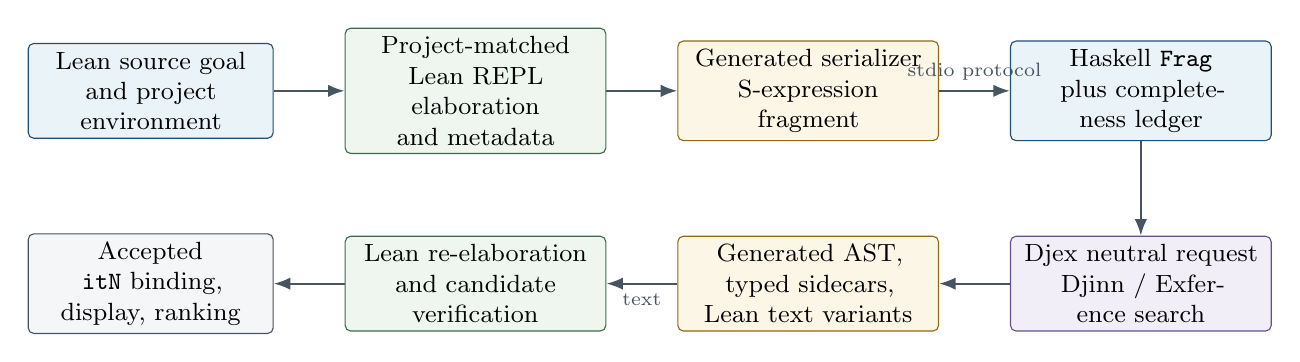
\begin{tikzpicture}[node distance=7mm and 9mm]
  \node[box,text width=29mm] (surface) {Lean source goal\\and project environment};
  \node[greenbox,right=of surface,text width=31mm] (elab) {Project-matched Lean REPL\\elaboration and metadata};
  \node[goldbox,right=of elab,text width=31mm] (sexp) {Generated serializer\\S-expression fragment};
  \node[box,right=of sexp,text width=31mm] (frag) {Haskell \code{Frag}\\plus completeness ledger};
  \node[purplebox,below=12mm of frag,text width=31mm] (djex) {Djex neutral request\\Djinn / Exference search};
  \node[goldbox,left=of djex,text width=31mm] (gen) {Generated AST, typed sidecars,\\Lean text variants};
  \node[greenbox,left=of gen,text width=31mm] (verify) {Lean re-elaboration\\and candidate verification};
  \node[graybox,left=of verify,text width=29mm] (present) {Accepted \code{itN} binding,\\display, ranking};

  \draw[flow] (surface) -- (elab);
  \draw[flow] (elab) -- (sexp);
  \draw[flow] (sexp) -- node[above,note]{stdio protocol} (frag);
  \draw[flow] (frag) -- (djex);
  \draw[flow] (djex) -- (gen);
  \draw[flow] (gen) -- node[below,note]{text} (verify);
  \draw[flow] (verify) -- (present);
\end{tikzpicture}}
\caption{Current positive-candidate path. Every arrow is intentional today, but several arrows exist only because the synthesis engine is in another language and process.}
\label{fig:current-roundtrip}
\end{figure}

This architecture has strong safety properties. A generated Haskell value cannot become a Lean declaration without Lean accepting it; a renderer bug is caught by re-elaboration; backend death does not silently preserve invalid environment IDs; and the synthesis engine cannot mutate Lean's environment directly. The cost is that exact semantic identity must be carried through a succession of representations that were never designed to be isomorphic.

\section{The fragment is three things, not merely a type AST}

The \code{Frag} language contains arrows, products, sums, top, bottom, forall binders, instance binders, exact class contexts, variables, opaque atoms, nominal applications, finite and recursive inductive descriptions, and a depth marker. Its fields retain more information than Djinn or Exference directly consumes. They collectively serve three roles:

\begin{enumerate}
  \item \term{Search projection.} The fragment determines which parts of an elaborated Lean type are represented structurally and which remain opaque.
  \item \term{Rendering guide.} Exact family names, constructor names, binder visibility, provider names, parameter vectors, and leading slots tell Haskell how to produce Lean source that refers to the original environment.
  \item \term{Completeness ledger.} Safe/unsafe atom bits, incomplete recursive descriptions, unsupported instance binders, and explicit depth exhaustion determine whether a candidate-free Djinn result may support a negative conclusion.
\end{enumerate}

This is an excellent design independent of implementation language. A Lean rewrite should retain these roles, but it need not encode them as quoted strings and then parse them back. A typed Lean structure can contain exact \code{Name}, \code{Level}, \code{BinderInfo}, inductive metadata, and local identifiers directly, while a deliberately smaller serializable projection can be derived only when a process or cache boundary requires it.

\section{Djex is a checked synthesis platform, not two old algorithms glued together}

The current package architecture in \dpath{docs/architecture.md} has four semantically relevant strata:

\begin{enumerate}
  \item a shared neutral synthesis foundation under \filepath{synthesis/src};
  \item the Djinn checked adapter, formula compiler, LJT search, proof checker, and lowerer;
  \item the Exference checked adapter, unifier, typed-hole search, scorer, and independent expression checker;
  \item the typed semantic stratum: candidate graphs, fingerprints, certificate associations, class resolution, Length contracts, concrete replay, SMT-LIB, and live Z3 process ownership.
\end{enumerate}

Historical Haskell frontends sit outside the needs of this report. The shared foundation is nevertheless essential. It prevents the two engines from assigning different meanings to names, kinds, provider assignments, declarations, generated terms, residual constraints, or search completion.

\subsection{Authority values are the dominant coding pattern}

Djex repeatedly constructs opaque values after validating all of the facts that downstream code is permitted to assume. Examples include checked environments, inventories, prepared inventories, cached queries, backend sessions, checked requests, typed candidates, sealed term graphs, certificate associations, Length contracts, interpreted problems, canonical SMT queries, executable policies, ready Z3 workers, and replay receipts.

This pattern is not Haskell-specific. In Lean it can be represented by private constructors, opaque definitions, indexed structures, subtypes, and proof fields. The important porting rule is to preserve the \emph{one-way authority acquisition}: downstream code may project validated facts, but it may not rebuild an authority from a printable view, a fingerprint string, or a structurally similar record.

\begin{designbox}
Do not translate opaque Haskell records into public Lean structures with freely constructible fields merely because Lean can attach propositions to them later. Keep constructors private and expose checked builders. Proof fields are useful where the property is stable and inexpensive to carry; module abstraction remains preferable for operational invariants involving IO handles, caches, process liveness, or expensive normalization.
\end{designbox}

\subsection{Finite observation and laziness are part of the contract}

The architecture document emphasizes that public Haskell trees contain lazy lists. Smart constructors cannot blindly call \code{length} on a caller-supplied spine because it may be cyclic or infinite. They perform bounded observation first. Conversely, search result tails remain lazy so a caller can obtain the first candidate without constructing the entire search space.

A Lean rewrite changes the accident but not the intent:

\begin{itemize}
  \item Lean's ordinary \code{List} is finite as a logical value, but runtime data can still be huge, partial computations can diverge, and streamed protocol input is not a pre-existing list. Width and resource bounds remain necessary.
  \item The Haskell pattern of a lazy list of search results should become an explicit cursor or resumable state machine. This makes progress, budget consumption, cancellation, and completion evidence more visible rather than less.
  \item Strict finite indexes should remain strict. Lean's arrays, hash maps, red-black maps, and functional-but-in-place optimizations are well suited to these tables.
\end{itemize}

\section{Djinn's trust story}

Djinn translates a supported neutral type problem to an intuitionistic propositional formula, explores a family of structural/nominal plans, searches an LJT-style calculus, normalizes proof terms, checks each proof independently, and lowers accepted proofs to the shared generated AST. It may produce negative evidence only when both the translation and the search are complete.

The noteworthy pieces for a rewrite are:

\begin{itemize}
  \item positive and negative forall occurrences are treated differently;
  \item nested unsupported polytypes become alpha-aware opaque atoms rather than strings;
  \item recursive families may expose a bounded constructor layer while retaining an opaque forwarding view;
  \item exact provider assignments become controlled instantiation premises only after source identity, kind, closure, and plan-retention checks;
  \item a candidate cutoff, choice-point bound, omitted plan, unsafe atom, or incomplete family description weakens a no-candidate result to ``undecided'';
  \item the proof checker is separate from the search procedure.
\end{itemize}

These are unusually good candidates for a Lean port. Formula syntax, sequents, proof terms, normalization, and checking are algebraic data and recursive functions. The existing independent checker supplies a natural executable specification. The completeness ledger can become a data type whose constructors name exactly which proof obligation remains missing.

\section{Exference's trust story}

Exference explores partial typed programs. A search node contains holes, expected types, scopes, flexible substitutions, rigid variables, givens, class obligations, global and local bindings, provider assignments, constructor/deconstructor data, usage counts, a generated expression, fresh supplies, a score, and depth/queue bookkeeping. The scheduler pops the most promising node, expands one selected hole, filters depth, checks solved nodes, scores future nodes, and merges them into a bounded queue with exact pruning counts.

It deliberately never turns empty-queue exhaustion into uninhabitability. A queue may be empty because of step limits, queue pruning, depth pruning, identifier exhaustion, disabled expansions, candidate policies, or an incomplete declaration projection. The independent expression checker reconstructs each solved expression and its residual constraints rather than trusting the search node's accumulated typing story.

Exference is the more demanding port, but not because it needs Haskell. The demanding properties are:

\begin{itemize}
  \item many persistent branch snapshots share large immutable substructures;
  \item the priority queue needs deterministic ordering and exact prune accounting;
  \item namespace-sensitive unification has several modes;
  \item rigid scopes and visible type applications carry origin information not reconstructible from a fully erased term;
  \item the result stream is incremental and bounded;
  \item candidate quality depends on allocation, scoring, and traversal behavior as well as type correctness.
\end{itemize}

Lean can represent all of these. The port should use a purpose-built immutable search state and explicit scheduler cursor, not Lean's global metavariable context as the authoritative branch representation. A metavariable context is excellent for final elaboration and local proof tactics, but it is tightly coupled to Lean internals, optimized for elaborator workflows, and awkward to serialize, fingerprint, compare, replay, and branch under Exference's exact policies.

\section{The semantic stratum changes the rewrite calculus}

The modern repositories contain much more than type-directed term generation. The documents \dpath{docs/semantic-foundations.md} and \lpath{docs/synth-internals.md} describe a large checked pipeline that associates an exact typed Exference candidate with a term graph, certificate origins, provider assumptions, a Length interpretation policy, a sealed candidate-specific problem, a canonical bounded QF\_LIA query, solver observations, and independently replayed counterexample receipts.

This layer is the main reason a naive ``port the old Djinn and Exference algorithms'' proposal is insufficient. The rewrite must preserve:

\begin{itemize}
  \item candidate-local identities that are not merely allocation numbers;
  \item graph/certificate association that is lost by a bare graph projection;
  \item exact provider-law bases and ground class discharge;
  \item policy and schema versions that are part of fingerprints;
  \item bounded canonical encodings and causal solver-response association;
  \item the rule that raw \code{sat}, \code{unsat}, and \code{unknown} strings have no authority by themselves;
  \item pure replay of model values against the exact sealed problem;
  \item explicit distinction between counterexample evidence, applicable-domain establishment, heuristic statuses, and no result.
\end{itemize}

A Lean implementation is a good fit for the pure parts of this stratum and opens significant verification opportunities. It also increases the importance of preserving opaque associations: dependent types can make an illegal state difficult to express, but careless serialization or an overly generic equality instance can still detach an authority from its exact candidate.

\section{Leant's recovery model is independent of Haskell}

Leant treats backend process state as a lease. Durable logical state consists of imports, replayable commands, snapshot artifacts, settings, and histories. Environment identifiers, process handles, provider serializations, and derived caches are process-local and are discarded after timeout or death. Replacement is transactional: reconstruct a complete session off to the side, then install it atomically.

This is one of the strongest current design choices and should survive a rewrite. Moving the controller into Lean does not make a project worker immortal, nor does it make arbitrary elaborator code safe to run in the controller process. The correct question is not ``can Lean hold an \code{Environment} value?'' but ``which process should own the environment whose failure policy the user expects?''

\begin{summarybox}
The current architecture contains both accidental and essential boundaries. Generated source, S-expression parsing, neutral-to-text rendering, and text-based semantic identity are accidental consequences of the language split. A project-local worker, independent candidate checking, explicit completeness evidence, solver replay, and transactional session reconstruction are essential trust and recovery boundaries.
\end{summarybox}

\chapter{Lean 4 capability fit}\label{ch:lean-fit}

\section{The relevant Lean execution layers}

A Lean-native Leant/Djex would use several distinct layers of Lean rather than treating ``Lean'' as one mechanism:

\begin{enumerate}
  \item \term{Pure executable data and functions}: inductive syntax, finite maps, arrays, unification, proof checking, scoring, fingerprints, SMT lowering, concrete evaluators, and protocol parsers.
  \item \term{Metaprogramming}: \code{MetaM}, \code{TermElabM}, and \code{CommandElabM} for reading the target expression, local context, environment declarations, type-class state, and pretty-printer metadata, and for lowering generated terms to \code{Expr}.
  \item \term{Kernel checking}: construction of a temporary declaration and checking it in a copied environment. Lean 4.33.0 exposes \code{Kernel.Environment.addDecl}; the ordinary \code{addDecl} path invokes the kernel unless explicitly configured to skip checking.
  \item \term{Runtime IO}: files, streams, tasks, cancellation checks, clocks, subprocesses, and signals. Lean's standard \code{IO.Process.spawn} supports piped stdin/stdout/stderr, working directories, child waiting, and termination.
  \item \term{C FFI}: only for platform primitives not represented by the standard runtime, most notably the current descriptor-bound Z3 launch policy if it is retained exactly.
\end{enumerate}

The official reference describes command elaborators as environment-modifying IO computations and term elaborators as computations that additionally inspect the local context and return a \code{Lean.Expr}. It separately distinguishes elaboration from trusted kernel checking. This maps almost exactly to Leant's desired ownership split: metaprogramming proposes and translates; the kernel accepts or rejects the final declaration.

\section{Subsystem feasibility matrix}

The following table evaluates the in-scope implementation, not historical Haskell compatibility layers. ``Benefit'' means the architectural benefit of placing the component in Lean rather than merely whether it can be ported.

\begin{longtable}{@{}L{0.22\textwidth}C{0.11\textwidth}C{0.13\textwidth}L{0.46\textwidth}@{}}
\toprule
\textbf{Subsystem} & \textbf{Feasibility} & \textbf{Lean benefit} & \textbf{Principal qualification} \\
\midrule
\endhead
Leant goal serializer / fragment builder & Very high & Very high & Directly consume elaborated \code{Expr}, exact \code{Name}, binder info, local declarations, inductive metadata, and levels; remove generated-source and S-expression round trip. \\
Provider and instance discovery & Very high & Very high & Must pin to the worker's Lean API version and preserve exact environment/provenance checks rather than trusting pretty names. \\
Neutral type/declaration/query layer & Very high & High & Keep a search-specific IR; do not collapse it into raw \code{Expr}. Lean indices/subtypes can strengthen selected invariants. \\
Djinn formula compiler & Very high & High & Formalizing polarity and completeness ledgers is attractive; recursive family and rank-N plans remain semantically intricate. \\
LJT search and proof normalization & Very high & Medium--high & Replace lazy proof streams with explicit cursors; use \code{partial} runtime code if necessary, while retaining a total checker. \\
Djinn independent proof checker & Very high & Very high & Natural target for a total function plus soundness theorem over the reified calculus. \\
Exference unification and scope model & High & High & Pure representation is straightforward; performance and persistent sharing need careful data-structure design. \\
Exference scheduler and priority queue & High & Medium & No semantic obstacle. Exact ordering/pruning and incremental results require an explicit scheduler state, not an incidental library heap. \\
Exference expression checker & Very high & Very high & Can remain independent of search and can additionally lower/check exact Lean expressions. \\
Generated term / typed term graph & Very high & Very high & Use exact global names and local identities; retain a neutral graph as authority and derive \code{Expr} plus presentation syntax. \\
Lean candidate rendering & Very high & Very high & Delaboration becomes presentation. Optional re-elaboration of displayed text remains useful for copy-paste fidelity. \\
Final candidate verification & Very high & Very high & A scratch declaration in a copied environment reaches the actual kernel. A mere \code{inferType} or successful unification is not an adequate replacement. \\
Length symbolic interpreter & Very high & High & Pure finite semantics is well suited to Lean and amenable to refinement/proof. \\
Applicable-domain validators & Very high & High & Their many bounded arithmetic cases can share generic checked traversals, as the current Haskell refactoring already suggests. \\
Typed QF\_LIA / SMT-LIB renderer & Very high & High & A typed AST and canonical renderer are conventional Lean code; canonicalization theorems are possible. \\
Incremental bounded SMT response parser & High & Medium--high & Lean has byte arrays and streams; preserve causal framing, byte/depth limits, and transaction ordinals. \\
Ordinary Z3 process session & Very high & Medium & Directly supported by \code{IO.Process.spawn}; still needs dedicated stdout/stderr draining and deadline policy. \\
Descriptor-bound/effective-ID Z3 launch & Medium in pure Lean; very high with C & Low as Lean code & Exact current semantics require OS calls below the standard API. Retain or rewrite the small C shim and expose an opaque Lean capability. \\
Leant controller / line-oriented UI & High & Medium & Basic IO is easy; matching Haskeline-quality editing may use a terminal library or FFI. This is a UX/library issue, not a semantic blocker. \\
Session replay, undo, reset, reload & Very high & Medium--high & Pure state accumulation and transactional replacement map cleanly to Lean structures and IO. \\
Snapshot sidecars/fingerprints & Very high & Medium & File and hashing logic is straightforward. \code{.olean} and tooling formats remain version-specific implementation details. \\
Cross-toolchain project worker & Very high & Very high & Build/cache the worker under the target project's Lake environment. Do not load foreign-version artifacts into the controller. \\
Differential and property tests & Very high & High & Retain fake-Z3/fault workers; use current Haskell as an oracle during migration. \\
\bottomrule
\end{longtable}

\section{Direct expression access removes several false authorities}

Today an exact Lean constant may successively appear as a pretty-printed string in the serializer output, an \code{AppNominal String} or provider name in \code{Frag}, a fresh private Haskell/Djex name during search, a mapping entry in the renderer, and a textual identifier in a candidate variant. Considerable code is devoted to proving that those views still denote the same declaration.

Inside a project worker, the authoritative representation can instead retain:

\begin{itemize}
  \item \code{Name} for global constants and constructors;
  \item \code{FVarId} or a worker-owned stable local ID for local binders;
  \item \code{BinderInfo} for explicit, implicit, strict implicit, and instance implicit positions;
  \item \code{Level} expressions or a normalized bounded level view where the search needs universe information;
  \item the exact \code{ConstantInfo} or an environment-generation stamp for lookup validation;
  \item constructor and inductive metadata obtained from the current environment;
  \item the source \code{Expr} as an inspection reference, never as the portable search state.
\end{itemize}

This does not eliminate all mappings. Djinn and Exference still require compact internal names and type variables; generated terms still require fresh local binders; fingerprints should remain independent of incidental allocation IDs. It does eliminate the need to recover declaration identity from text.

\begin{findingbox}
The largest semantic benefit of Lean is not dependent types in the abstract. It is the ability to keep exact Lean identities alive from target inspection through candidate lowering, so that strings become display values rather than authority tokens.
\end{findingbox}

\section{Kernel-checking a generated candidate}

A Lean-native verifier should use a stricter pipeline than ``\code{Meta.inferType} returned the expected expression.'' A suitable conceptual sequence is:

\begin{enumerate}
  \item instantiate all assigned metavariables and reject any remaining expression or universe metavariables;
  \item check that every free variable belongs to the captured local context and that no local declaration has escaped its scope;
  \item abstract the local context into a closed type and value, preserving binder information and dependency order;
  \item create a fresh private theorem or definition declaration whose type is the abstracted expected type and whose value is the abstracted candidate;
  \item call the synchronous kernel declaration checker on a copied environment, with kernel checking explicitly enabled;
  \item discard the copied environment unless the candidate is committed as an \code{itN} definition;
  \item independently delaborate for display; optionally re-elaborate the displayed text in the original context to establish copy-paste fidelity.
\end{enumerate}

Illustrative pseudocode:

\begin{lstlisting}[language=Leanish]
structure CheckedCandidate where
  expr        : Lean.Expr
  expected    : Lean.Expr
  origin      : CandidateOrigin
  kernelStamp : KernelCheckStamp

-- Sketch, not a literal current API wrapper.
def kernelCheckCandidate
    (env : Lean.Environment)
    (lctx : Lean.LocalContext)
    (candidate expected : Lean.Expr) : MetaM CheckedCandidate := do
  let candidate <- instantiateMVars candidate
  let expected  <- instantiateMVars expected
  unless !candidate.hasMVar && !expected.hasMVar do
    throwError "candidate contains unresolved metavariables"
  let (closedType, closedValue) <- abstractLocalContext lctx expected candidate
  let decl <- mkPrivateTheoremDecl closedType closedValue
  let _checkedEnv <- kernelAddDeclSynchronously env decl
  pure { expr := candidate, expected, origin := ..., kernelStamp := ... }
\end{lstlisting}

The final stamp must not be a caller-constructible Boolean. It should be returned only by the checker and should bind the candidate, expected type, environment/toolchain identity, and relevant options. A fingerprint can be a view of that association, not a constructor for it.

In Lean 4.33.0 each step of the sketch has a concrete counterpart, and the details explain two of the report's insistences. Metavariables are resolved with \code{instantiateMVars} and universe metavariables generalized with \code{abstractMVars}; the local context is abstracted with \code{mkForallFVars} for the type and \code{mkLambdaFVars} for the value, which preserve binder information and dependency order. The scratch environment is obtained with \code{withoutModifyingEnv}, which restores the previous environment when the block exits. The check itself is \code{Kernel.Environment.addDecl env opts decl}, whose first line consults \code{debug.skipKernelTC} and, when that option is set, silently calls \code{addDeclWithoutChecking}; this is why the verifier must pin the option off in the options it passes rather than inheriting them. Finally, the ordinary \code{Lean.addDecl} in \code{CoreM} may add a constant asynchronously through \code{addConstAsync}, deferring the kernel check to a task; the acceptance decision must therefore either call the synchronous \code{Kernel.Environment.addDecl} directly or await the environment's checked task before answering, which is the ``synchronous'' requirement repeated in \autoref{ch:trust} and the risk register.

\section{Why the search IR should not be raw \code{Expr}}

The temptation in a Lean rewrite is to remove both Haskell and Djex's neutral type language and search directly in Lean's expression/metavariable machinery. That would gain access to definitional equality and type-class synthesis, but it would sacrifice several properties the current system works hard to maintain:

\begin{itemize}
  \item a small, auditable fragment with an explicit completeness ledger;
  \item stable equality and alpha-normal fingerprints independent of elaborator allocation IDs;
  \item deterministic serialization and differential testing;
  \item independent checking rather than replaying search mutations;
  \item exact accounting of steps, choices, queue pruning, and structural plans;
  \item the ability to keep unsupported dependent regions opaque without accidentally normalizing them under an aggressive reducibility mode;
  \item decoupling of the search algorithms from changes in Lean's metavariable implementation.
\end{itemize}

The right replacement is a \term{Lean-oriented neutral IR}. It may use Lean's \code{Name}, binder kinds, and exact declaration handles at the worker boundary, but its recursive structure and substitution rules remain owned by Djex. The current \code{Frag} and shared \code{Type} should probably converge into fewer representations in Lean, yet they should not vanish into \code{Expr}.

A practical split is:

\begin{lstlisting}[language=Leanish]
/-- Exact worker-side reference, never serialized across toolchains. -/
structure LeanOrigin where
  envGeneration : UInt64
  sourceExpr    : Lean.Expr
  sourceType    : Lean.Expr
  globals       : Array Lean.Name

/-- Pure search problem; serializable, fingerprintable, and checker-owned. -/
structure PreparedProblem where
  fragment      : Fragment
  declarations  : Inventory
  providers     : Array ProviderBinding
  completeness  : CompletenessLedger
  origin        : LeanOrigin
\end{lstlisting}

The exact \code{Expr} fields are useful for final lowering and diagnostics. The pure fragment remains the object on which search and completeness claims are defined.

\section{Explicit search cursors replace ambient laziness}

Djinn and Exference expose incremental results today through Haskell laziness. Lean should make the continuation explicit:

\begin{lstlisting}[language=Leanish]
inductive SearchStep (Candidate State : Type) where
  | yield   (candidate : Candidate) (next : State)
  | advance (next : State)
  | done    (completion : Completion)

def SearchCursor.next : SearchCursor -> SearchM (SearchStep Candidate SearchCursor)
\end{lstlisting}

For Djinn, a cursor can retain the current plan index, sequent-search continuation, global choice budget, candidate cutoff witness state, and deduplication set. For Exference, it can retain the priority queue, counters, exact pruning totals, fresh-supply ceiling, and pending checked candidates. This design has several benefits:

\begin{itemize}
  \item cancellation checks occur at explicit administrative steps;
  \item serialization of a cursor can be prohibited or supported intentionally;
  \item completion evidence is produced only by the \code{done} constructor;
  \item profiling can distinguish search work from checking and presentation;
  \item no caller accidentally forces a large tail by applying an innocent-looking list function.
\end{itemize}

The loss is syntactic convenience and perhaps some fusion. Given the importance of exact progress semantics, the explicit form is arguably clearer than the current lazy-list encoding.

\section{Lean's proof language helps, but only at the right layer}

Several correctness properties can be stated and proved in Lean:

\begin{itemize}
  \item the LJT proof checker is sound with respect to a semantics of the reified formula language;
  \item proof normalization preserves checked typing;
  \item selected formula-compiler rules preserve inhabitation under explicit assumptions;
  \item substitution and alpha-normalization preserve well-scopedness;
  \item the Exference expression checker accepts only well-typed neutral terms;
  \item canonical SMT rendering and parsing preserve the typed QF\_LIA plan;
  \item concrete replay of a model receipt really violates the sealed Length contract under the stated provider laws;
  \item finite-domain validators cover exactly the assignments they claim to cover.
\end{itemize}

Other properties remain difficult even after a rewrite:

\begin{itemize}
  \item completeness of the entire rank-N plan family for all admitted Lean goals;
  \item correctness of the metaprogram that projects arbitrary Lean \code{Expr} into the fragment;
  \item semantic adequacy of treating selected opaque atoms as propositional variables;
  \item completeness of recursive-family exposure policies;
  \item equivalence between an external provider summary and the actual Lean definition's behavior;
  \item correctness of Z3 itself when no independently checkable proof certificate is consumed.
\end{itemize}

\begin{trustbox}
A Lean implementation can make more claims checkable, but language choice is not a proof. Search code may be \code{partial}, use IO, call Z3, or contain bugs. The sound positive boundary remains a kernel-checked candidate; semantic claims require replay or certificates; negative claims require a proved or audited completeness chain.
\end{trustbox}

\section{Process and FFI support}

Lean's process API is sufficient for the ordinary worker and Z3 paths. It can spawn asynchronously with piped handles, set a working directory and environment, write incrementally, read stdout/stderr, wait, poll, and terminate. Its task system supports cooperative cancellation; long pure loops must call cancellation checks explicitly or be enclosed by a killable worker process.

The FFI is also sufficient to retain the existing C helper. The current Lean reference warns that the FFI is still designed largely for internal use and should be considered unstable. That is a maintenance risk, but the required surface can be extremely small: pass a validated path/policy descriptor to C, receive inherited pipe handles and a process identifier or a structured error, then hide the raw values behind an opaque Lean \code{Z3ProcessCapability}.

\begin{riskbox}
Do not move the entire Z3 protocol into C merely because a C shim is retained. Keep policy validation, command bytes, deadlines, response framing, causal transaction state, and replay in Lean. The C layer should perform only the primitive launch operation that Lean's standard library cannot express with the required guarantees.
\end{riskbox}

\section{Performance is an empirical risk, not a feasibility barrier}

Lean 4 is designed as an efficient functional language and compiles to native code. It supports arrays, hash tables, tasks, compact algebraic data, and functional-but-in-place optimization. There is no reason in principle that Djinn or Exference must be slower. There are, however, specific places where the current GHC behavior should not be assumed to transfer automatically:

\begin{itemize}
  \item Haskell's pervasive sharing of immutable branch states versus Lean array/map update behavior;
  \item garbage-collector behavior under a wide Exference priority queue;
  \item cost of proof-bearing dependent records if overused in inner loops;
  \item hash and comparison costs for large canonical types/graphs;
  \item loss of lazy producer/consumer fusion in result streams;
  \item interaction between long search tasks and Lean's heartbeat/cancellation accounting;
  \item debug versus optimized native builds of metaprograms loaded into a project worker.
\end{itemize}

The remedy is architectural: keep proofs out of hot nodes when a sealed checked constructor suffices; use compact numeric IDs internally; preserve immutable authority at boundaries; use mutable arrays locally under \code{ST}/IO where uniqueness permits; and benchmark candidate quality, not only wall-clock time. Exference's search ordering can change when allocation or queue tie-breaking changes even if every candidate remains type-correct.

\begin{summarybox}
Lean 4 supplies every capability needed for the semantic rewrite: exact elaborator access, efficient native functional code, kernel declaration checking, tasks, subprocesses, binary IO, and C interoperability. The porting risks are performance engineering, API version coupling, and preserving authority boundaries---not expressiveness.
\end{summarybox}

\chapter{Full-rewrite architecture choices}\label{ch:full-architectures}

A full rewrite can take several forms. They share the same synthesis core but differ in where the Lean environment lives, how a search is cancelled, and how the user invokes it.

\section{Variant A: native tactic, term elaborator, and command}

In the most Lean-native form, the package exposes interfaces such as:

\begin{lstlisting}[language=Leanish]
-- Insert a term synthesized for the expected type.
syntax "leant" : term

-- Inspect/rank candidates and show them without committing one.
syntax (name := leantQuery) "leant?" : tactic

-- Standalone command for a fully elaborated target.
syntax "#leant " term : command
\end{lstlisting}

The engine runs in the same Lean server process as the current file. It sees the exact local context and environment with no protocol at all. Accepted candidates can be assigned to the current metavariable or added as declarations. Editor integration can attach messages, goals, candidate previews, term graphs, and counterexample data to source ranges.

\subsection{Advantages}

\begin{itemize}
  \item maximal access to the current local context, open namespaces, options, reducibility settings, and declarations;
  \item no separate session language or manual replay for ordinary use;
  \item direct return of \code{Expr}, with no need to create a printable candidate before use;
  \item natural integration with the Lean language server, widgets, tactic traces, and source positions;
  \item the project automatically compiles the package against its own Lean toolchain;
  \item users can invoke synthesis at an actual proof hole, not only at a standalone REPL prompt.
\end{itemize}

\subsection{Disadvantages}

\begin{itemize}
  \item a long or allocating search competes with elaboration and editor responsiveness;
  \item cooperative cancellation depends on the search checking cancellation often enough;
  \item a runtime crash, FFI failure, or severe memory blow-up can take down the Lean server process;
  \item Leant's current free-form REPL, undo model, and snapshot UX do not map one-to-one onto a tactic;
  \item a worker that runs Z3 and reads configuration files inside elaboration must be disciplined about deterministic diagnostics and source replay;
  \item keeping multiple expensive search sessions alive across commands requires environment extensions or external state whose lifecycle must cooperate with incremental recompilation.
\end{itemize}

This variant is highly desirable as an \emph{interface}, but it should not necessarily execute the entire search in-process. A tactic can prepare the exact goal, send a pure prepared problem to a local worker, and kernel-check the returned expression in the server.

\section{Variant B: Lean controller plus project-local Lean worker}

This is the recommended standalone architecture. A small controller executable owns the terminal UI, settings, durable history, configuration acquisition, worker discovery/build, fault handling, and replacement policy. A worker executable is compiled under the target project's Lake environment and owns the Lean environment, elaboration, provider discovery, Djex search, candidate lowering, kernel checking, and optional Z3 session.

\begin{figure}[H]
\centering
\resizebox{0.97\textwidth}{!}{%
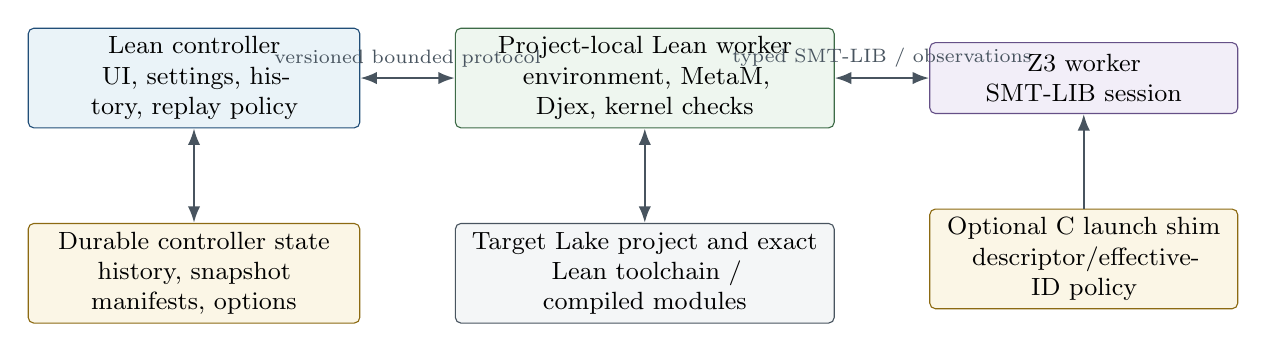
\begin{tikzpicture}[node distance=8mm and 12mm]
  \node[box,text width=40mm] (controller) {Lean controller\\UI, settings, history, replay policy};
  \node[greenbox,right=of controller,text width=46mm] (worker) {Project-local Lean worker\\environment, MetaM, Djex, kernel checks};
  \node[purplebox,right=of worker,text width=37mm] (z3) {Z3 worker\\SMT-LIB session};
  \node[goldbox,below=12mm of z3,text width=37mm] (cshim) {Optional C launch shim\\descriptor/effective-ID policy};
  \node[graybox,below=12mm of worker,text width=46mm] (project) {Target Lake project and exact\\Lean toolchain / compiled modules};
  \node[goldbox,below=12mm of controller,text width=40mm] (durable) {Durable controller state\\history, snapshot manifests, options};

  \draw[bothflow] (controller) -- node[above,note]{versioned bounded protocol} (worker);
  \draw[bothflow] (worker) -- node[above,note]{typed SMT-LIB / observations} (z3);
  \draw[flow] (cshim) -- (z3);
  \draw[bothflow] (worker) -- (project);
  \draw[bothflow] (controller) -- (durable);
\end{tikzpicture}}
\caption{Recommended full rewrite. Language unification removes semantic representation crossings, while process separation preserves toolchain and fault boundaries.}
\label{fig:recommended-architecture}
\end{figure}

\subsection{Controller responsibilities}

The controller should know as little as possible about Lean expressions. It owns:

\begin{itemize}
  \item terminal input, command history, color, selection, and high-level display policy;
  \item project discovery and worker build/cache selection;
  \item protocol framing, request IDs, deadlines, stdout/stderr capture, process termination, and replacement;
  \item durable user settings and imported configuration source bytes;
  \item a replay log of successful user commands and stable snapshot manifests;
  \item presentation of worker-produced structured diagnostics and candidate views;
  \item no authority to declare a candidate well-typed, a goal uninhabited, or a solver observation valid.
\end{itemize}

The controller can be compiled with one Lean version because it never loads the target project's \code{.olean} files. Its protocol types should be kept in a small compatibility package or generated schema. If controller and worker versions differ, the handshake selects a common protocol version or fails before session creation.

\subsection{Worker responsibilities}

The worker owns everything tied to the target toolchain:

\begin{itemize}
  \item imports and current \code{Environment};
  \item elaboration of commands and synthesis targets;
  \item exact local/global identity and provider discovery;
  \item fragment preparation and completeness ledger;
  \item Djinn and Exference sessions, searches, checkers, and candidate authorities;
  \item direct lowering to \code{Expr};
  \item kernel checking and committing accepted \code{itN} declarations;
  \item delaboration and optional text round-trip checks;
  \item typed semantic graphs, Length problem sealing, replay, and live Z3 policy;
  \item process-local caches keyed by environment generation and exact policy identity.
\end{itemize}

A worker crash loses only process-local state. The controller reconstructs a replacement from a snapshot/import root and replay log, exactly as current Leant does. The rewrite can simplify the protocol because the worker no longer needs to send a fragment to a Haskell engine and receive text back; synthesis can remain inside the worker.

\subsection{Why the worker should include Djex rather than spawn it separately}

A three-process architecture---controller, Lean elaboration worker, and synthesis engine---would preserve additional isolation but would reintroduce a large serialization boundary between exact Lean preparation and search. The recommended default is to compile Djex into the project worker. This allows exact names and typed origin handles to remain in memory and makes direct \code{Expr} lowering possible.

A separate synthesis process remains useful as an optional hard sandbox for untrusted experimental search policies. In that mode, the Lean worker should send only a sealed neutral problem and receive a neutral candidate plus evidence. The Lean worker remains responsible for origin resolution and kernel checking. No raw \code{Expr}, environment pointer, or process-local certificate handle crosses the boundary.

\section{Variant C: one standalone Lean process}

A single Lean executable can load project imports, provide the REPL, run both engines, manage Z3, and hold all state. This is feasible and is the smallest conceptual program. It is also the least attractive replacement for current Leant.

The one-process design couples:

\begin{itemize}
  \item UI responsiveness to elaboration and search memory use;
  \item recovery logic to whether the process survived;
  \item project toolchain compatibility to the executable's build;
  \item terminal state to foreign library and solver failures;
  \item durable history to in-memory \code{Environment} identity.
\end{itemize}

It can be appropriate for a project-specific executable built by Lake, where restarting the whole program is cheap and no cross-project controller is required. It should not be the only supported architecture.

\section{Variant D: native tactic with an out-of-process search service}

This variant combines editor-native invocation with strong search isolation:

\begin{enumerate}
  \item the tactic/term elaborator reads the exact goal and builds a sealed neutral problem;
  \item a long-lived worker service searches that problem and returns neutral candidates/evidence;
  \item the tactic resolves exact origins, lowers the candidate to \code{Expr}, and kernel-checks it;
  \item the editor receives structured candidates or counterexamples.
\end{enumerate}

It is a strong secondary target. The service can be the same project-local worker used by the standalone controller, with a protocol request that carries a local-context snapshot encoded in the neutral IR. Local free variables need stable occurrence IDs and exact types, not serialized Lean heap objects.

\section{Recommended product shape}

The most coherent end state exposes both of the following over one core:

\begin{itemize}
  \item \term{Leant package}: \code{leant}, \code{leant?}, and command APIs for normal Lean/editor use;
  \item \term{Leant standalone}: a Lean controller that starts a project-local worker and preserves the current exploratory REPL, history, undo, snapshots, ranking controls, and diagnostics.
\end{itemize}

The in-process package may initially run small Djinn searches directly and delegate expensive Exference/Length/Z3 work to the worker. The standalone controller always delegates to the worker. Both consume the same checked result types and final kernel-verification path.

\chapter[Recommended Lean-native module architecture]{Recommended Lean-native\\module architecture}\label{ch:recommended-architecture}

\section{Package decomposition}

A Lean rewrite should use Lake packages or libraries that reflect semantic ownership rather than historical repository provenance. One possible layout is:

\begin{longtable}{@{}L{0.31\textwidth}L{0.61\textwidth}@{}}
\toprule
\textbf{Module family} & \textbf{Responsibility} \\
\midrule
\endhead
\filepath{Djex/Core/Name} & Validated internal/global/local identities and canonical source mappings. \\
\filepath{Djex/Core/Kind} & Ground kinds, universe-erased search kinds, bounded inference, and exact positional evidence. \\
\filepath{Djex/Core/Type} & Neutral monotypes/polytypes, constraints, alpha-aware atoms, substitution, canonical views, and free-variable analysis. \\
\filepath{Djex/Core/Environment} & Opaque checked declaration environment and deterministic indexes. \\
\filepath{Djex/Core/Query} & Cached query preflight, checked request envelopes, options, progress, and evidence. \\
\filepath{Djex/Core/Generated} & Neutral expressions, patterns, visible type applications, scope checking, simplification, and candidate envelopes. \\
\filepath{Djex/Djinn/*} & Formula compiler, structural plans, LJT cursor, normalization, proof checker, lowering, and negative-evidence ledger. \\
\filepath{Djex/Exference/*} & Types, unification, scopes, node builder, scheduler, scoring, expression checker, and typed graph production. \\
\filepath{Djex/TypedGraph/*} & Stable graph identities, certificate tables, exact associations, canonical fingerprints, and checked projections. \\
\filepath{Djex/Semantic/Length/*} & Contracts, interpretation policies, provider summaries, candidate problems, concrete evaluation, applicable-domain validators, and receipts. \\
\filepath{Djex/SMT/*} & Typed QF\_LIA, canonical rendering, bounded response parsing, causal stream, query fingerprints, replay, and observations. \\
\filepath{Djex/Z3/*} & Execution policies, sessions, deadlines, readiness, process owner, and the optional C-shim binding. \\
\filepath{Leant/Meta/Fragment} & Direct \code{Expr}-to-fragment projection, exact Lean origin table, refusal/completeness information. \\
\filepath{Leant/Meta/Providers} & Library/provider discovery, active-instance evidence, premise construction, and environment-generation caches. \\
\filepath{Leant/Meta/Lower} & Neutral generated term to exact Lean \code{Expr}; constructor, binder, and visible-application restoration. \\
\filepath{Leant/Meta/Verify} & No-metavariable checks, abstraction, scratch declaration creation, kernel checking, and display round-trip. \\
\filepath{Leant/Synth} & Portfolio orchestration, result merging, exact-text/view deduplication, ranking, and acceptance. \\
\filepath{Leant/Session} & Environment generations, replay, undo, snapshots, reset/reload/load, and transactional replacement. \\
\filepath{Leant/Protocol} & Bounded controller/worker messages, version negotiation, diagnostics, and stable presentation views. \\
\filepath{Leant/Worker} & Project-local executable and request dispatcher. \\
\filepath{Leant/Controller} & Toolchain-neutral executable, terminal UX, worker lifecycle, durable state, and recovery. \\
\filepath{Leant/Elab} & Native term/tactic/command entry points and optional editor integration. \\
\bottomrule
\end{longtable}

Djex can remain a separate repository/library if independent reuse and clean layering are valuable. Because the only target is Lean, its public vocabulary should no longer be named \code{Language.Haskell.*}, but it should still avoid depending on Leant's UI/session modules. The reusable boundary is ``checked synthesis over a Lean-oriented neutral problem,'' not ``Haskell source synthesis.''

\section{A three-level identity model}

The current repositories repeatedly distinguish source identity, search identity, and display spelling. The Lean design should make this explicit.

\begin{enumerate}
  \item \term{Lean identity}: exact \code{Name}, local declaration identity, environment generation, and source \code{Expr}. Valid only inside one worker/toolchain/session generation.
  \item \term{Neutral semantic identity}: stable variable/global/constructor/provider IDs in a checked inventory; serializable and fingerprintable; independent of Lean heap allocation.
  \item \term{Presentation identity}: delaborated syntax, qualified spelling, candidate ordinal, renderer route, and UI grouping. Never sufficient to recover an authority.
\end{enumerate}

A mapping from Lean identity to neutral identity is created during preparation and retained in a private origin table. Lowering uses the inverse mapping only after the neutral candidate has passed its engine checker. Presentation is derived last.

\begin{lstlisting}[language=Leanish]
structure OriginTable where
  envGeneration : EnvGeneration
  globals        : Array Lean.Name
  constructors   : Array Lean.Name
  locals         : Array Lean.FVarId
  providers      : Array ProviderOrigin

structure PreparedOrigin where
  problem : NeutralProblem
  table   : OriginTable
  -- private constructor: problem IDs are guaranteed to index this table
\end{lstlisting}

The neutral problem may be sent to a separate search service. The origin table must remain in the Lean worker; a remote candidate refers only to checked neutral IDs.

\section{Converging \code{Frag} and Djex's shared type without losing roles}

Current Leant first builds \code{Frag}, then \lpath{src/Leant/Synth/Engine.hs} translates it into Djex declarations/types. A Lean rewrite can reduce duplication by defining one reified type language with annotations:

\begin{lstlisting}[language=Leanish]
inductive Fragment where
  | var          (id : TyVarId)
  | atom         (id : AtomId) (safety : AtomSafety)
  | app          (head : TypeHead) (args : Array Fragment)
  | arr          (domain codomain : Fragment)
  | product      (kind : ProductKind) (left right : Fragment)
  | sum          (kind : SumKind) (left right : Fragment)
  | top | bottom
  | forallE      (binder : TypeBinder) (body : Fragment)
  | instanceE    (binder : InstanceBinder) (body : Fragment)
  | exactContext (ctx : ExactClassApplication) (body : Fragment)
  | inductive    (family : FamilyRef) (args : Array Fragment)
  | depthLimit   (path : FragmentPath)
\end{lstlisting}

Backend-specific compilers then view this common tree:

\begin{itemize}
  \item Djinn derives polarity-aware formula plans and nominal constructor descriptions;
  \item Exference derives schemes, constructor/deconstructor bindings, rigid scopes, and provider choices;
  \item the Lean lowerer consults exact source metadata associated with IDs;
  \item the completeness analysis folds over the same nodes and records reasons;
  \item semantic domains inspect only supported typed graph nodes, not source fragments.
\end{itemize}

Not every current \code{Frag} distinction should be erased. For example, saturated Lean \code{Prod} may need a different behavioral adapter from proposition-valued \code{And}; exact instance contexts are not ordinary arrows; recursive family completeness is separate from its constructor inventory; and an opaque atom's refutation safety is not implied by its text.

\section{Candidate authority and views}

The end-to-end candidate should have one authoritative object with lossy views, mirroring the best parts of current Exference sidecars:

\begin{lstlisting}[language=Leanish]
opaque CheckedNeutralCandidate : Type

structure LeanCandidateView where
  expr          : Lean.Expr
  expectedType  : Lean.Expr
  display       : Syntax
  pretty        : String
  rendererRoute : RendererRoute

structure SemanticCandidateView where
  graph         : Option BareTermGraph
  absence       : Option GraphAbsenceReason

opaque AcceptedCandidate : Type

def CheckedNeutralCandidate.lower
    (origin : PreparedOrigin)
    (candidate : CheckedNeutralCandidate) : MetaM LeanCandidateView

def verifyAndAccept
    (origin : PreparedOrigin)
    (candidate : CheckedNeutralCandidate)
    (view : LeanCandidateView) : MetaM AcceptedCandidate
\end{lstlisting}

The bare graph projection remains intentionally weaker than a graph/certificate association. Equality and ordering used for display deduplication must not silently choose between an authority-bearing candidate and a plain equivalent view. The current warning in Djex's typed-candidate design remains applicable in Lean: containers keyed by a lossy equality can discard the representative that carries the authority.

A safe rule is to finish ranking and display deduplication over explicit keys, then retain a separate variant-scoped pointer to the exact typed origin. Do not define \code{BEq} or \code{Ord} on the opaque authority merely for convenience.

\section{Portfolio orchestration}

Djinn and Exference should remain separate engines behind one portfolio API:

\begin{lstlisting}[language=Leanish]
inductive Engine where | djinn | exference

structure EngineResult where
  candidates : SearchCursor CheckedNeutralCandidate
  progress   : Progress
  evidence   : EngineEvidence
  notes      : Array Diagnostic

structure PortfolioResult where
  groups     : Array CandidateGroup
  negative   : Option NegativeEvidence
  progress   : PortfolioProgress
\end{lstlisting}

The merge policy must preserve the current asymmetry:

\begin{itemize}
  \item Exference candidates can improve ranking and library use;
  \item Exference failure cannot create or cancel a logical refutation;
  \item Djinn negative evidence survives only if the fragment/compiler/search completeness chain is intact;
  \item duplicate displayed text may retain the first exact Exference semantic origin without transferring that origin to a Djinn candidate;
  \item wrappers such as classical transformations create a new term and must drop origins that no longer denote the exact graph.
\end{itemize}

Direct \code{Expr} candidates permit a stronger semantic deduplication key than exact text, but it should be introduced cautiously. Alpha-equivalence, binder-name changes, reducible constants, eta, and proof irrelevance all offer possible quotients; each can merge terms with different behavioral graphs or provider occurrences. Exact normalized neutral-tree identity is the safe default. Text remains useful as the user's observed grouping key.

\section{The worker protocol}

The controller/worker protocol should be versioned and bounded, but much smaller than today's combined Lean-REPL plus Haskell-synthesis protocols. Representative request classes are:

\begin{itemize}
  \item session creation, import root, and capability handshake;
  \item execute command and return new environment generation/history record;
  \item synthesize current expression/declared target with engine and ranking policy;
  \item accept a specific candidate by opaque session-local candidate token;
  \item inspect candidate details, graph, diagnostics, or counterexample receipt;
  \item snapshot/restore, reload, reset, and health probe;
  \item cancel request and terminate worker.
\end{itemize}

Large internal values should not be serialized merely because a protocol exists. Candidate tokens are process-local leases. A candidate listing returns bounded presentation data and stable fingerprints; acceptance sends the token back to the same worker, which still owns the exact candidate and origin. After worker death, tokens are invalid and synthesis must be rerun or reconstructed from a durable neutral cache whose schema explicitly supports it.

\begin{designbox}
Use the protocol to preserve fault and toolchain isolation, not to expose every internal record. The best protocol is capability-oriented: the worker owns exact environments and candidates; the controller owns durable user intent and refers to worker objects by generation-bound tokens.
\end{designbox}

\section{Z3 placement}

The Z3 session can live inside the project worker because Length candidate authority is already there. It may also be delegated to a separate generic solver service, but then the service must receive only a canonical SMT query and return raw bounded observations. The project worker independently parses, associates, and replays those observations against its sealed problem.

This preserves the existing rule:

\[
\text{solver output} \quad\neq\quad \text{semantic evidence}
\]

Only:

\[
\text{sealed candidate problem}
+ \text{canonical query}
+ \text{associated bounded observation}
+ \text{independent replay}
\]

can produce a counterexample receipt. A separate Z3 service therefore does not need access to Lean, provider inventories, term graphs, or Length contracts.

\section{Snapshots and environment generations}

The worker should attach a monotonically fresh \code{EnvGeneration} to every committed environment state. All process-local caches, prepared origins, candidate tokens, provider inventories, and exact declarations are indexed by that generation. Undo may restore an older environment object while creating a new generation token, avoiding accidental reuse of stale capabilities.

Durable snapshots retain:

\begin{itemize}
  \item the project/toolchain identity;
  \item root imports or a compatible \code{.olean} family;
  \item tooling ABI/schema fingerprints;
  \item replay history after the root;
  \item settings that affect semantic preparation and ranking;
  \item no raw \code{Expr}, \code{FVarId}, environment pointer, process handle, candidate token, or certificate carrier.
\end{itemize}

The current publication/validation discipline---temporary files, exact siblings, versioned sidecar, sizes/fingerprints, rollback on partial publication---should be ported essentially unchanged.

\begin{summarybox}
The recommended rewrite is a Lean-native semantic core embedded in a project-local worker, not a monolithic process. Exact Lean identities stay inside the worker; the search uses a stable neutral IR; candidates remain opaque authorities with lossy views; the controller holds durable intent and process policy; and Z3 remains an untrusted observation source.
\end{summarybox}

\chapter{Rewriting Djinn in Lean}\label{ch:djinn}

\section{Feasibility verdict}

Djinn is the easiest major engine to justify rewriting in Lean. Its core objects are finite syntax, proof terms, translation plans, sequent states, and explicit evidence. The current architecture already separates an untrusted search procedure from a proof checker. Lean can preserve that separation and additionally host machine-checked metatheory for the reified calculus.

\begin{verdictbox}[title={Djinn verdict}]
A complete Lean rewrite is highly feasible and strongly advisable. It offers the clearest formal-verification payoff and removes no valuable Haskell-specific abstraction. The main design work is an explicit replacement for lazy proof streams and a precise account of which translation plans support negative evidence.
\end{verdictbox}

\section{Formula compiler}

The compiler should remain a separate phase from proof search. Its output is not merely a formula; it is a package containing:

\begin{itemize}
  \item one reified formula or a finite plan family;
  \item constructor descriptions and nominal identities required for lowering;
  \item opaque atom identities and alpha-normal source keys;
  \item opened/skolemized forall sites;
  \item exact provider-instantiation premises and their source occurrence paths;
  \item recursive-family exposure decisions;
  \item a completeness classification and exact reasons for incompleteness.
\end{itemize}

A Lean representation can make the last field more informative than a Boolean:

\begin{lstlisting}[language=Leanish]
inductive IncompletenessReason where
  | unsafeOpaqueAtom      (atom : AtomId)
  | serializerDepth       (path : FragmentPath)
  | unsupportedDependency (path : FragmentPath)
  | omittedForallPlan     (site : ForallSite)
  | partialRecursiveView  (family : FamilyId)
  | unsupportedInstance   (path : FragmentPath)
  | premiseProjectionLoss (provider : ProviderId)
  | boundedPlanFamily     (bound : Nat) (remaining : Nat)

deriving Repr, DecidableEq

structure CompileResult where
  plans   : Array FormulaPlan
  reasons : Array IncompletenessReason

def CompileResult.complete (r : CompileResult) : Bool := r.reasons.isEmpty
\end{lstlisting}

This does not prove the compiler correct, but it makes accidental promotion of an incomplete result harder. The type returned by exhaustive search can require a \code{CompleteCompilation} witness built only when the reason array is empty and all local plan obligations are discharged.

\section{LJT search as a resumable machine}

The current continuation-encoded lazy search distinguishes yielded proofs, administrative progress, and branch completion. A Lean port should retain that operational distinction explicitly. One useful design is a small-step machine:

\begin{lstlisting}[language=Leanish]
structure LJTMachine where
  work       : WorkQueue
  budget     : ChoiceBudget
  freshness  : FreshSupply
  statistics : LJTStatistics

inductive LJTEvent where
  | proof    (term : ProofTerm) (next : LJTMachine)
  | stepped  (next : LJTMachine)
  | exhausted (summary : ExhaustionSummary)
  | truncated (reason : TruncationReason)

def LJTMachine.step : LJTMachine -> LJTEvent
\end{lstlisting}

Depth-first and fair-interleaving strategies become different \code{WorkQueue} implementations or transition policies. The global choice budget belongs to the machine, not to individual plans. The candidate cutoff observes one additional checked proof when necessary to establish that a tail was truly truncated.

Explicit machines also make the following invariants testable:

\begin{itemize}
  \item every transition consumes the exact documented choice count;
  \item fairness-specific queue rotation does not duplicate or lose work;
  \item freshening never reuses a live binder ID;
  \item administrative steps cannot be mistaken for exhaustion;
  \item a truncated plan cannot contribute to global negative evidence;
  \item the plan scheduler shares global budgets rather than resetting them.
\end{itemize}

\section{Proof checker and possible formalization}

The checker should be a total recursive function over a proof term and formula environment, returning either a derivation object or a structured error. A minimal executable interface is:

\begin{lstlisting}[language=Leanish]
inductive CheckError where
  | unknownVariable ...
  | expectedImplication ...
  | expectedConjunction ...
  | expectedDisjunction ...
  | constructorMismatch ...
  | binderEscape ...

opaque CheckedProof (ctx : Context) (goal : Formula) : Type

def checkProof (ctx : Context) (goal : Formula) (term : ProofTerm) :
    Except CheckError (CheckedProof ctx goal)
\end{lstlisting}

Internally, \code{CheckedProof} may contain the term and a proposition establishing a declarative typing judgment. There are two viable proof depths:

\begin{enumerate}
  \item \term{Executable checker with a soundness theorem.} Define an inductive judgment \(\Gamma \vdash p : A\), prove \code{checkProof} returns only derivable terms, and prove derivable formulas semantically valid. This is relatively direct.
  \item \term{Verified decision procedure.} Prove the LJT search complete and terminating for the exact formula fragment and strategy. This is much more ambitious because current plan scheduling, fairness adjustments, nominal constructor descriptions, and budget variants must be separated from the pure calculus theorem.
\end{enumerate}

A sensible architecture proves the calculus and checker first, then treats the search as an untrusted proof producer. Positive soundness no longer depends on the search implementation. Negative evidence continues to depend on either a completeness theorem for an unbudgeted search machine or an audited exhaustiveness argument.

\section{Formula semantics and Lean terms}

The reified formula semantics can be interpreted into Lean propositions or types:

\begin{align*}
\llbracket A \to B \rrbracket &= \llbracket A \rrbracket \to \llbracket B \rrbracket,\\
\llbracket A \land B \rrbracket &= \llbracket A \rrbracket \times \llbracket B \rrbracket,\\
\llbracket A \lor B \rrbracket &= \operatorname{Sum}\,\llbracket A \rrbracket\,\llbracket B \rrbracket.
\end{align*}

However, the search formula's atoms are not generally Lean propositions with directly available interpretations. They may denote arbitrary \code{Sort u} values, opaque dependent applications, or nominal family occurrences. The compiler/lowerer therefore needs an environment assigning each atom and constructor description an exact Lean type/constant.

For positive candidates, no global theorem connecting the whole compiler to Lean is required for soundness: lower the checked proof to an exact Lean expression and let the kernel verify it. For negative evidence, the connection is essential. ``No proof in the abstract formula'' implies ``no Lean inhabitant'' only if the projection is complete in the relevant direction.

This is why a Lean rewrite should resist an attractive but false slogan: \emph{the LJT checker is verified, therefore a no-proof result proves the Lean type empty}. The metatheory of the reified calculus and the adequacy of the Lean-to-fragment projection are separate.

\section{Positive lowering}

Current Djinn lowering restores constructor identities, tuple structure, source names, provider instantiations, and visible type applications into the common generated AST. A Lean-native lowerer can either produce the neutral generated AST and then \code{Expr}, or lower directly from a checked proof through a structured intermediate.

The intermediate remains useful because:

\begin{itemize}
  \item it can be independently scope-checked;
  \item it is serializable for differential tests;
  \item simplification and deduplication should operate before Lean-specific elaborator effects;
  \item the same typed graph/fingerprint machinery can consume it;
  \item failures can identify whether proof lowering or Lean expression construction was responsible.
\end{itemize}

The final Lean lowerer should construct applications, lambdas, lets, recursor/case expressions, constructors, and visible type arguments using exact constants and local declarations. Surface tuple or pattern syntax is unnecessary for semantic lowering. Delaboration can choose a pleasant display form afterward.

\section{Rank-N and impredicative instantiation}

This remains the most subtle part of the Djinn port. The current engine does not generally decompose negative foralls. It opens selected positive sites, preserves unsupported sites as opaque atoms, and creates exact instantiation premises only from checked evidence. Plan families explore open/opaque choices under explicit bounds.

Lean's own dependent type theory does not remove this issue. Djinn is still a propositional search engine. Direct access to \code{Expr} lets the compiler identify binder structure more accurately, but it does not make impredicative proof search complete.

The Lean implementation should encode each instantiation premise with:

\begin{itemize}
  \item the exact provider/source identity;
  \item the original forall telescope;
  \item the selected argument vector and each ground kind;
  \item a proof/check result that substitution is capture-free and closed in the admitted scope;
  \item the occurrence path retained by the current structural plan;
  \item the exact visible-application evidence required during lowering.
\end{itemize}

A synthetic logical axiom used by search must never be convertible into an arbitrary source call by name alone. Lowering consumes the checked premise object and emits the corresponding exact Lean application.

\section{Recursive data}

Recursive family exposure should remain bounded and dual:

\begin{itemize}
  \item an opaque view permits forwarding a value without infinite unfolding;
  \item a one-layer constructor view permits introduction and selected elimination;
  \item exact family identity prevents structurally similar nominal types from being conflated;
  \item completeness records whether all constructors and fields were represented;
  \item any approximation that makes the search problem easier poisons negative evidence unless formally justified.
\end{itemize}

Lean metadata can improve exactness because the worker can inspect the inductive declaration, parameters, indices, recursor, constructor field dependencies, and recursive occurrences directly. It should still reject or opaque dependent/indexed forms that the neutral calculus cannot faithfully represent.

\section{Negative evidence in a Lean rewrite}

There are three possible strengths of negative result:

\begin{enumerate}
  \item \term{Operational exhaustion}: the machine completed the admitted plan family without a proof. This is an internal fact, not yet a Lean theorem.
  \item \term{Verified formula unprovability}: a verified decision procedure establishes that the reified formula has no proof. This is stronger, but still about the reified problem.
  \item \term{Kernel-level source uninhabitability}: Lean accepts a theorem such as \code{IsEmpty T} or \code{Not (Nonempty T)} for the original target. This requires an adequacy bridge and is not automatically derivable from intuitionistic nonprovability of an arbitrary type.
\end{enumerate}

Current Leant's honest labels should remain. A Lean rewrite can gradually promote more cases to the second or third category. For example, a fully reified proposition built only from \code{False}, \code{True}, \code{And}, \code{Or}, and nondependent arrows over exact proposition variables may admit a reflection theorem. Arbitrary \code{Type}-valued atoms and recursive nominal data require a more careful semantic model.

\section{Djinn-specific advantages and disadvantages}

\begin{longtable}{@{}L{0.18\textwidth}L{0.74\textwidth}@{}}
\toprule
\textbf{Side} & \textbf{Details} \\
\midrule
\endhead
Advantages & Direct exact Lean origin metadata; simpler lowering; a total checker with formal soundness; explicit completeness types; no Haskell source concepts; easier generation of proof terms/certificates; shared definitions between executable checker and metatheory; native integration with tactics. \\
Disadvantages & Explicit cursor machinery replaces elegant laziness; proof-heavy inner data can harm compile/runtime performance if over-indexed; Lean API changes affect fragment preparation; proving full search completeness is substantial; direct access to definitional equality can tempt unsoundly broad normalization relative to the declared fragment. \\
Neutral factors & The core algorithm and asymptotic search space do not improve merely by changing language; opaque atoms, rank-N bounds, recursive exposure, and candidate explosion remain. \\
\bottomrule
\end{longtable}

\begin{summarybox}
Djinn should be the first search engine ported. It has the cleanest executable specification, the strongest benefit from proof objects, and the weakest dependence on Haskell runtime behavior. Its Lean rewrite can improve positive trust immediately while preserving current negative-result conservatism until compiler/search adequacy is formally established.
\end{summarybox}

\chapter{Rewriting Exference in Lean}\label{ch:exference}

\section{Feasibility verdict}

Exference is fully implementable in Lean, but it is the subsystem most likely to expose performance and representation mistakes. Its semantics are not difficult for Lean's type system; its operational workload is demanding: many persistent branches, frequent unification and substitution, a bounded priority queue, exact counters, and independent reconstruction of solved terms.

\begin{verdictbox}[title={Exference verdict}]
A complete rewrite is feasible and advisable as part of a Lean-first system. It should follow the neutral core and Djinn port, retain a pure branch-state model, and be benchmarked differentially against the current engine. Do not replace it with ad hoc Lean metavariable search merely to shorten the port.
\end{verdictbox}

\section{Search-node representation}

The current Exference node is deliberately self-contained. A Lean node should retain the same principle while separating shared immutable context from branch-local deltas:

\begin{lstlisting}[language=Leanish]
structure ExferenceStatic where
  inventory       : PreparedInventory
  globals         : Array GlobalBinding
  constructors    : Array ConstructorBinding
  deconstructors  : Array DeconstructorBinding
  classEnv        : ClassEnvironment
  providerEvidence: ProviderEvidence
  scoringPolicy   : ScoringPolicy

structure ExferenceNode where
  holes          : PersistentMap HoleId TypedGoal
  selected       : HoleId
  expression     : AnnotatedExpr
  substitution   : Substitution
  scopes         : ScopeForest
  localBindings  : PersistentMap LocalId LocalBinding
  givens         : PersistentMap ScopeId (Array Constraint)
  usage          : PersistentMap BindingId Nat
  fresh          : FreshSupplies
  depth          : Nat
  scoreState     : ScoreState
\end{lstlisting}

Every node need not copy \code{ExferenceStatic}. A session/cursor can own it and nodes can contain only stable IDs. Within a node, maps whose updates are frequent should be chosen by measured workload rather than by the most mathematically elegant API. Possibilities include persistent red-black maps, hash maps with copy-on-write arrays, or branch-local delta chains periodically compacted.

\subsection{Avoid proof-indexing hot state}

It is possible to define a node indexed by the exact set of holes, scopes, and typing judgments so that many invalid transitions are unrepresentable. That is unlikely to be a good runtime design. The number of dependent equality transports would increase elaboration complexity and compiled term size, while the independent checker already provides the correct trust boundary.

Use dependent types selectively:

\begin{itemize}
  \item \code{Fin} or checked compact IDs for array bounds;
  \item private constructors for substitutions and scope forests;
  \item proof fields for cheap local facts such as a nonempty selected-hole array;
  \item ordinary checked transitions for global typing consistency;
  \item a total independent checker for accepted candidates.
\end{itemize}

This follows the current architecture's separation between a fast speculative search and a slower authoritative check.

\section{Unification}

Exference's unifier has multiple namespace modes: two schemes may use disjoint IDs; a local and global type may share rigid variables; one side may contain the only bindable variables. A Lean port should encode these modes as explicit input tags or typed wrappers, not a Boolean flag:

\begin{lstlisting}[language=Leanish]
inductive UnificationMode where
  | disjoint
  | sharedRigids
  | bindLeft
  | bindRight

structure TaggedType where
  origin : TypeOrigin
  type   : Type

def unify (mode : UnificationMode)
    (left right : TaggedType) : Except UnifyError Substitution
\end{lstlisting}

Before unification, variables are injected into a disjoint tagged namespace. The occurs check sees free variables inside opaque polytype atoms without structurally decomposing their forall. Higher-kinded head binding checks ground kind arity. Substitution is simultaneous and capture-avoiding.

This is fertile ground for formal properties:

\begin{itemize}
  \item applying a successful substitution makes the two types alpha-equivalent;
  \item the substitution does not bind a prohibited namespace;
  \item no binding contains its own variable under the declared occurs relation;
  \item kind checking is preserved;
  \item substitution into an opaque atom preserves lexical hygiene.
\end{itemize}

A verified most-general-unifier theorem is possible for the first-order subset, but the immediate value is a shared executable unifier used by both search and the independent checker, with property tests and a small soundness lemma suite.

\section{Scopes, rigids, and visible type applications}

Lean provides exact local contexts and universe levels, but Exference's neutral scope model should remain explicit. It needs to represent search-created binders and branches before any Lean \code{FVarId} exists. A scope forest can assign each scope a parent and each local binder an introduction scope. A use is valid when its binder scope is an ancestor of the use scope.

Rigid variables require both a type-level identity and a provenance scope. A candidate may not let a rigid introduced while opening one provider's forall escape into a sibling branch or result. Visible type applications additionally carry whether an argument was inferred, specified from exact evidence, or selected by a bounded query-derived lane.

The annotated neutral expression should retain this origin until checking and typed-graph construction finish. Erasing it early and trying to infer it from the final Lean expression would recreate the authority-recovery problem the current code explicitly avoids.

\section{Scheduler and queue}

The scheduler should be a deterministic pure state machine with an explicit queue abstraction:

\begin{lstlisting}[language=Leanish]
structure ScheduledNode where
  score : Score
  tie   : StableTieBreaker
  node  : ExferenceNode

opaque BoundedQueue : Type

def BoundedQueue.merge
    (capacity : Nat)
    (old : BoundedQueue)
    (new : Array ScheduledNode) : Prod BoundedQueue Nat
\end{lstlisting}

The returned \code{Nat} is the exact number pruned by the merge. It must not be reconstructed by comparing queue sizes after deduplication or by assuming which input lost entries. Depth-pruned children are counted separately. Stable tie breakers should derive from deterministic search identities, not pointer addresses, hash iteration order, or runtime task scheduling.

Possible queue implementations include a pairing heap, binomial heap, binary heap over an array, or a sorted bounded vector for small capacities. The current scoring/queue sizes should drive the choice. A mutable binary heap inside one scheduler state is compatible with functional architecture if node values are immutable and the heap is not shared across cursors. Search branching occurs in nodes, not in the global queue owner.

\section{Expansion functions}

Each expansion family should have a narrow signature that consumes one selected typed goal and returns checked child deltas or a structured refusal:

\begin{lstlisting}[language=Leanish]
inductive ExpansionKind where
  | introduceArrow
  | introduceForall
  | applyLocal
  | applyGlobal
  | applyProvider
  | constructTuple
  | constructData
  | eliminateTuple
  | eliminateData
  | introduceLet

structure ExpansionContext where
  static : ExferenceStatic
  node   : ExferenceNode
  goal   : TypedGoal

def expand (kind : ExpansionKind)
    (ctx : ExpansionContext) : ExpansionResult
\end{lstlisting}

An expansion must update expression, holes, substitution, scopes, constraints, usage, fresh supplies, and score inputs atomically. Returning a public partial record invites inconsistent nodes. A private \code{NodeDelta} can be applied only by one checked constructor.

Provider application deserves its own path. It consumes exact occurrence-local assignments, substitutes a complete binder vector, introduces visible type applications where required, and records certificate/source annotations for the typed graph. Ordinary implicit instantiation remains a different lane; exact evidence is not flattened into a scalar candidate pool.

\section{Independent expression checker}

The checker is the most important Exference component to port faithfully. It should reconstruct a neutral expression bidirectionally against an opaque context:

\begin{itemize}
  \item validate local scope and global exact identity;
  \item infer/check applications, lambdas, tuples, lets, constructors, and cases;
  \item replay forall introduction and visible type application;
  \item check rigid provenance and nonescape;
  \item resolve class givens and residual constraints;
  \item verify exact provider assignments and certificate annotations;
  \item compare reconstructed residual constraints with the claimed set;
  \item reject holes, stale IDs, duplicate pattern binders, and malformed graph annotations.
\end{itemize}

The checker should return a \code{CheckedNeutralCandidate}, not a Boolean. Typed-graph construction may happen during checking because the checker is the authoritative source of node types and application origins. If graph sealing or certificate association fails, the candidate may remain valid for Lean lowering while its semantic graph is unavailable with a precise reason.

The final Lean lowerer and kernel checker form an additional independent layer. Thus a candidate passes:

\[
\text{Exference search}
\longrightarrow
\text{neutral expression checker}
\longrightarrow
\text{Lean lowering}
\longrightarrow
\text{kernel declaration checker}.
\]

This is stricter than using Lean's elaborator as the only checker and preserves backend-independent diagnostics.

\section{Relationship to Lean type-class synthesis}

A Lean rewrite gains access to the live instance environment. It may be tempting to let Lean synthesize all class obligations during search. That should be done carefully.

Lean instance synthesis can serve three roles:

\begin{enumerate}
  \item \term{Preparation authority}: establish that a ground provider context is actually dischargeable in the current environment, then record the exact instance result/provenance allowed by policy.
  \item \term{Final elaboration}: fill ordinary implicit instance arguments in a candidate expression, subject to the expected source semantics.
  \item \term{Search heuristic}: suggest useful providers or ground facts.
\end{enumerate}

It should not silently replace Djex's checked class environment in the middle of a neutral search. Doing so would make search behavior depend on ambient metavariable state, reducibility, local instance priority, and potentially nonterminating type-class search. The neutral engine should consume a bounded prepared inventory. When exact Lean instance synthesis is needed, perform it at a named boundary and retain the result as checked evidence.

\section{Typed term graph in Lean}

The term graph should remain a neutral graph rather than simply storing \code{Expr}. It needs stable occurrence IDs, exact types, visible-argument witnesses, local binding structure, case order, holes/absence reasons, and certificate associations. A canonical fingerprint deliberately ignores allocation numbers while preserving semantic structure.

A Lean port can strengthen graph sealing:

\begin{itemize}
  \item use compact \code{Fin nodeCount} IDs after construction;
  \item validate all child and occurrence references in one pass;
  \item store the graph in topological or source order only as an implementation detail;
  \item define canonical rooted-tree encoding independently of table order;
  \item prove or test that reindexing preserves the canonical encoding;
  \item separate a bare graph projection from a certificate-associated carrier at the type level.
\end{itemize}

For example:

\begin{lstlisting}[language=Leanish]
opaque SealedGraph : Type
opaque AssociatedGraph : Type

def SealedGraph.bareView : SealedGraph -> BareGraph

def associateCertificates
    (graph : SealedGraph)
    (table : CheckedCertificateTable)
    (observations : Array CheckerOriginObservation) :
    Except AssociationError AssociatedGraph

-- Deliberately no function BareGraph -> AssociatedGraph.
\end{lstlisting}

The associated graph is retained inside the typed candidate. Its public equality need not exist. Fingerprints that require association authority accept \code{AssociatedGraph}, while generic structural fingerprints accept only a graph proven free of certificate-bearing nodes or a complete associated carrier.

\section{Performance plan}

A credible rewrite should benchmark at least the following separately:

\begin{itemize}
  \item node expansion rate by family;
  \item allocation and peak live memory per queued node;
  \item unification and substitution cost by type size and forall depth;
  \item queue merge cost and exact pruning at realistic capacities;
  \item independent-checker cost per solved node;
  \item typed-graph sealing/fingerprinting cost;
  \item candidate order and top-\(k\) quality under identical policies;
  \item cancellation latency and worker termination cleanup.
\end{itemize}

Differential tests should compare semantic traces, not raw internal IDs. A normalized trace can contain selected expansion kind, neutral goal fingerprint, score tuple, prune counts, checked candidate fingerprint, and completion reason. This allows the Lean implementation to use different data structures while detecting meaningful ordering drift.

\section{What should not be ported}

The Haskell-specific Exference frontend includes Haskell source extraction, workspace loading, source renderers, historical command APIs, and compatibility expression constructors. None is needed. The Lean rewrite should also remove any neutral distinction whose sole purpose is reproducing Haskell surface syntax, while retaining distinctions necessary for:

\begin{itemize}
  \item Lean implicit/explicit binder behavior;
  \item exact universe/kind treatment;
  \item nominal inductive identity;
  \item type-class contexts;
  \item visible type applications;
  \item provider and certificate provenance;
  \item semantic term graphs.
\end{itemize}

\section{Exference-specific advantages and disadvantages}

\begin{longtable}{@{}L{0.18\textwidth}L{0.74\textwidth}@{}}
\toprule
\textbf{Side} & \textbf{Details} \\
\midrule
\endhead
Advantages & Exact Lean provider/constructor identities; direct lowering; native instance preparation; one language for checker, graph, and semantic domains; opportunity to prove unifier/checker properties; deletion of Haskell source frontends; easier tactic/editor integration. \\
Disadvantages & Greater performance uncertainty than Djinn; explicit replacement for lazy result traces; need for carefully chosen persistent/mutable data structures; temptation to couple to unstable Lean Meta internals; large compile times if hot state is over-indexed with proofs. \\
Neutral factors & Heuristic incompleteness, score tuning, queue/depth bounds, candidate explosion, and the inability to infer uninhabitability remain intrinsic. \\
\bottomrule
\end{longtable}

\begin{summarybox}
Exference is not a reason to retain Haskell permanently. It is a reason to preserve the current algorithmic boundaries and to stage the port behind differential traces and performance gates. Its independent checker and typed graph should move with the search engine as one semantic unit.
\end{summarybox}

\chapter{Rewriting the typed semantic and Z3 strata}\label{ch:semantic}

\section{Feasibility verdict}

The typed semantic layer is large, but most of it is particularly well suited to Lean: finite typed graphs, checked contracts, symbolic interpretation, arithmetic expressions, bounded traversal, canonical encodings, concrete evaluation, and replay receipts. The difficult part is not the mathematics; it is preserving exact association and lifecycle policy across many opaque values.

\begin{verdictbox}[title={Semantic/Z3 verdict}]
Rewrite the semantic layer in Lean together with Exference's typed candidate authority. Rewrite the SMT protocol, parser, replay, and session owner in Lean. Retain a narrow C shim only for the current hardened descriptor-bound launch mode; use Lean's ordinary process API for portable/default execution.
\end{verdictbox}

\section{Keep candidate identity atomic}

The current system has learned, through several iterations, that a candidate's printable term, bare graph, certificate table, provider inventory, policy, and candidate key cannot be independently reconstructed and then assumed to match. The Lean rewrite should encode a pipeline of consumption rather than a collection of public records:

\begin{lstlisting}[language=Leanish]
opaque TypedCandidate : Type
opaque LengthSession : Type
opaque LengthContract : Type
opaque SealedLengthProblem : Type
opaque CanonicalQuery : Type
opaque SolverObservation : Type
opaque CounterexampleReceipt : Type

def LengthSession.sealCandidateProblem
    (session : LengthSession)
    (contract : LengthContract)
    (candidate : TypedCandidate) :
    Except LengthRefusal SealedLengthProblem

def SealedLengthProblem.toCanonicalQuery
    (p : SealedLengthProblem) : Except QueryRefusal CanonicalQuery

def replayObservation
    (q : CanonicalQuery)
    (obs : SolverObservation) :
    Except ReplayRefusal (Option CounterexampleReceipt)
\end{lstlisting}

There should be no public constructor from:

\begin{itemize}
  \item a graph fingerprint to a typed candidate;
  \item a list of provider names to a provider-law authority;
  \item raw SMT bytes to a canonical query;
  \item a \code{sat} token and model values to a counterexample receipt;
  \item a printed candidate plus ordinal to an exact typed origin.
\end{itemize}

Each transition checks the exact predecessor and consumes or retains its authority.

\section{Length contracts and symbolic interpretation}

The Length domain interprets finite list-spine behavior over selected input/result roles. It supports exact case policies, provider summaries, conditional contexts, zero/step behavior, finite products, and a growing family of applicable-domain validators. A Lean implementation can model the contract as a closed syntax with checked role indices:

\begin{lstlisting}[language=Leanish]
structure LengthContractSource where
  arity       : Nat
  roles       : Array TargetRole
  precondition: LengthPredicate arity
  postcondition : LengthPredicate (arity + 1)
  casePolicy  : CasePolicy
  domain      : RankingDomain   -- scalar or binary-product; the file carries no version

opaque LengthContract (arity : Nat) : Type

def checkLengthContract
    (limits : ContractLimits)
    (src : LengthContractSource) :
    Except ContractError (Sigma LengthContract)
\end{lstlisting}

The exact dependent indexing can be internal. Public JSON/configuration parsing may first produce untrusted naturals and arrays, then a checked constructor validates lengths and converts indexes to \code{Fin arity}.

The symbolic interpreter consumes a checked typed graph and exact provider summaries. It should return a symbolic expression plus a used-law basis and a complete interpretation trace. Provider names are display metadata; used-law identity is derived from the exact checked summary object selected at each global occurrence.

\section{Formalization opportunity: interpreter soundness}

A high-value theorem is local rather than universal:

\begin{quote}
For a sealed candidate graph interpreted under a checked provider-law environment, every concrete input assignment satisfying the precondition and every provider implementation satisfying the named summaries produces output lengths described by the generated arithmetic relation.
\end{quote}

The theorem can be parameterized by provider laws instead of proving those laws for arbitrary Lean definitions. This matches the current conditional trust model. It would establish that a replayed arithmetic counterexample is a valid counterexample to the candidate under those assumptions.

The proof can be staged:

\begin{enumerate}
  \item define concrete evaluation of the neutral term graph over abstract spine lengths;
  \item define symbolic evaluation into arithmetic expressions/relations;
  \item prove one rule at a time (lambda/application, constructors, selected case forms, provider calls);
  \item prove the used-law set contains every provider assumption invoked;
  \item prove evaluation of the symbolic relation agrees with concrete graph evaluation;
  \item layer contract pre/postconditions and role selection on top.
\end{enumerate}

Unsupported nodes return a refusal, not a default symbolic value. This fail-closed behavior is easier to prove than a total interpreter with approximation flags.

\section{Applicable-domain validators}

The repository now contains many solver-independent validators: direct literal bounds, positive-affine variants, relational and strict relational forms, quotient/extrema/monus variants, Boolean finite unions, atomic branching, and recursive piecewise-affine families. Recent refactoring unifies public validators behind generic ladders.

Lean is a good host for further consolidation. A generic validator can be parameterized by:

\begin{itemize}
  \item a recognized predicate grammar;
  \item an extractor producing a finite domain descriptor;
  \item a proof/check result that the descriptor covers every satisfying assignment within the admitted semantics;
  \item a bounded enumerator;
  \item an evaluator and violation predicate;
  \item a receipt constructor containing the descriptor and complete traversal count.
\end{itemize}

A validator that cannot prove/check coverage returns \code{inapplicable}; it does not fall back to incomplete enumeration and call success ``established.'' Nullary domains and vacuous preconditions retain explicit semantics.

The most useful proof target is:

\[
\text{validator returns Established}
\implies
\forall x \in D_{\text{applicable}},\; \text{contract holds at }x.
\]

This theorem depends only on the finite evaluator and coverage witness, not on Z3.

\section{Typed QF\_LIA and canonical rendering}

The current system constructs a typed plan before rendering SMT-LIB and includes the plan in a complete structural fingerprint. The Lean port should retain a typed arithmetic AST:

\begin{lstlisting}[language=Leanish]
inductive LIAExpr (n : Nat) where
  | input  (i : Fin n)
  | lit    (value : Int)
  | add    (xs : Array (LIAExpr n))
  | sub    (a b : LIAExpr n)
  | mulLit (k : Int) (a : LIAExpr n)
  | ite    (c : LIAPred n) (t e : LIAExpr n)

inductive LIAPred (n : Nat) where
  | le | lt | eq
  | and | or | not
  -- with checked operands omitted here
\end{lstlisting}

Canonicalization should be explicit and versioned. The renderer emits only from the canonical AST. A parser for Djex's own canonical bytes is not required for live use, but a decoder can support durable fixtures and independent round-trip tests. The fingerprint includes schema version, variable order, assertions, requested observations, and all limits that affect admissibility.

\section{Bounded response parsing and causal association}

Z3 stdout is an untrusted byte stream. The current causal stream distinguishes lexical framing, transaction ordinals, readiness, and the exact command whose response is being interpreted. A Lean parser should operate incrementally over \code{ByteArray}, with limits on:

\begin{itemize}
  \item total buffered bytes and bytes per transaction;
  \item token/string length;
  \item parenthesis depth and list width;
  \item numeral digit count;
  \item number of model/value entries;
  \item diagnostic lines retained;
  \item transactions per session and usable-work budget.
\end{itemize}

The parser produces a raw response syntax, not evidence. The causal driver then associates it with the pending transaction type:

\begin{lstlisting}[language=Leanish]
inductive PendingTransaction where
  | capabilityProbe ...
  | checkSat       (query : CanonicalQuery)
  | getValues      (query : CanonicalQuery) (symbols : Array InputSymbol)
  | exit

opaque AssociatedObservation : Type

def associate
    (pending : PendingTransaction)
    (raw : RawResponse) : Except ProtocolError AssociatedObservation
\end{lstlisting}

A model response arriving after a timed-out or cancelled query cannot be reassigned to the next query. Killing the worker on ambiguous protocol state remains the safest policy.

\section{Live session and usable-work budgets}

One Z3 process may serve a bounded batch of candidate queries. The session authority should retain:

\begin{itemize}
  \item exact executable identity/policy and capability probe result;
  \item process handles and liveness state;
  \item the next command/observation ordinal;
  \item absolute deadline and per-run remaining budget;
  \item total admitted usable work;
  \item current transaction state and buffered bytes;
  \item solver options that affect semantics or output;
  \item a fingerprint of the complete execution policy.
\end{itemize}

A raw process handle is not a ready session. Readiness follows a bounded capability probe and exact identity check. A session that has encountered framing ambiguity, unexpected output, deadline expiry during a transaction, or child death is poisoned and cannot be reused.

Lean tasks can drain stdout and stderr concurrently. The session owner should not rely on finalizers for timely cleanup; use lexical ownership with \code{try/finally}, explicit close/kill/wait, and a small state machine preventing double termination.

\section{Descriptor-bound launch and the C boundary}

Djex's \filepath{synthesis/cbits/z3_descriptor_spawn.c} is not an arbitrary native optimization. It implements launch semantics that the ordinary process API does not expose: binding execution to a previously opened descriptor and checking effective-ID accessibility/identity according to the selected policy. The Haskell owner additionally associates the resulting process with derived policy fingerprints and readiness evidence.

There are three possible Lean rewrite choices:

\begin{enumerate}
  \item \term{Preserve exact semantics with C FFI.} Port or retain the C helper, expose one checked Lean call, and keep all policy validation and process ownership in Lean. Recommended when hardening is a requirement.
  \item \term{Use ordinary \code{IO.Process.spawn}.} Simpler and portable; sufficient for most local tooling. Executable path resolution/identity has weaker time-of-check/time-of-use guarantees. This is a conscious policy downgrade.
  \item \term{Extend Lean's runtime.} Add the primitives upstream or in a custom runtime layer. This can produce a pure Lean call site, but the implementation is still C/C++ and carries a larger maintenance surface than a package-local shim.
\end{enumerate}

The FFI function should accept a compact, already validated policy structure and return a result that cannot be forged from integers:

\begin{lstlisting}[language=Leanish]
opaque SpawnedZ3 : Type

@[extern "djex_spawn_z3_descriptor_bound"]
private opaque spawnZ3Primitive
    (path : @& String)
    (policyBits : UInt32)
    (stdinFd stdoutFd stderrFd : UInt32) : IO PrimitiveSpawnResult

def spawnCheckedZ3
    (policy : CheckedExecutablePolicy) : IO SpawnedZ3 := ...
\end{lstlisting}

Raw file descriptors should not escape the module. The wrapper converts them immediately into owned handles or closes them on every failure path.

\section{Counterexample receipts and proof strength}

A replayed Length counterexample establishes a bounded model-relative fact under provider assumptions. It is not automatically:

\begin{itemize}
  \item an executable Lean input value of the original polymorphic types;
  \item a theorem that the candidate violates a Lean proposition;
  \item evidence that Z3's \code{unsat} response is correct;
  \item a reason to prune all structurally related candidates;
  \item transferable to a candidate with the same printed text but a different typed origin.
\end{itemize}

A Lean rewrite should keep receipt names honest. A possible hierarchy is:

\begin{lstlisting}[language=Leanish]
opaque ArithmeticCounterexampleReceipt : Type
opaque ConcreteGraphCounterexampleReceipt : Type
opaque LeanCounterexampleWitness : Type

-- Pure replay against the sealed symbolic problem.
def replayArithmetic ... : Option ArithmeticCounterexampleReceipt

-- Requires a proved interpreter correspondence for the supported graph.
def liftToGraph ... : Option ConcreteGraphCounterexampleReceipt

-- Requires construction/evaluation of actual Lean values or a kernel theorem.
def realizeInLean ... : MetaM (Option LeanCounterexampleWitness)
\end{lstlisting}

This allows future proof strength to increase without relabeling today's model-level evidence.

\section{Offline first, live second}

The semantic API should preserve a strict separation:

\begin{itemize}
  \item pure sealing of candidate problems;
  \item pure canonical query generation;
  \item pure replay of supplied observations/inputs;
  \item solver-independent finite validation;
  \item optional live Z3 execution only after all eligible queries are sealed.
\end{itemize}

This ordering has operational and proof benefits. It discovers refusals before spawning a process, makes configuration and fingerprints deterministic, permits replay banks and offline tests, and ensures a live solver never grants authority unavailable to the pure API.

\section{Advantages and disadvantages}

\begin{longtable}{@{}L{0.18\textwidth}L{0.74\textwidth}@{}}
\toprule
\textbf{Side} & \textbf{Details} \\
\midrule
\endhead
Advantages & Shared definitions between typed graph, interpreter, replay, and proofs; stronger impossible-state prevention; direct candidate association; removal of Haskell serialization glue; formalizable finite-domain validators and interpreter rules; Lean-native process/session integration; better editor display of receipts. \\
Disadvantages & Large API surface to port faithfully; C FFI remains for strongest launch mode; Lean FFI is officially unstable; byte-stream parsers and concurrent process cleanup require careful low-level testing; overuse of dependent indexing can make configuration/schema code cumbersome. \\
Neutral factors & Z3 remains external and untrusted; provider summaries remain assumptions unless separately proved; \code{unknown} remains meaningful; solver heuristics and query complexity do not improve automatically. \\
\bottomrule
\end{longtable}

\begin{summarybox}
The semantic stratum should be seen as a prime reason to move to Lean, not a reason to stay in Haskell. Its pure checked transformations can gain formal guarantees and share exact candidate identities with the search/checking layer. The low-level launch shim is a narrow exception that should remain narrow.
\end{summarybox}

\chapter{Rewriting Leant itself}\label{ch:leant}

\section{Feasibility verdict}

Leant's synthesis-specific code benefits greatly from Lean because it currently reconstructs Lean identity and syntax across a Haskell boundary. Its standalone REPL/session code is also feasible in Lean, but its best properties come from process architecture rather than language. A rewrite should therefore be selective in design, even if complete in implementation language.

\begin{verdictbox}[title={Leant verdict}]
Rewrite the Lean-facing synthesis bridge, renderer/lowerer, verification, provider preparation, and native tactic interfaces in Lean. Reimplement the standalone controller in Lean only if eliminating Haskell at runtime is a goal; preserve the external project worker and transactional replay model. Do not place durable UI state and arbitrary project elaboration in one process by default.
\end{verdictbox}

\section{Direct fragment preparation}

The generated serializer in \lpath{src/Leant/Synth/Fragment.hs} can become an ordinary \code{MetaM} function. This removes:

\begin{itemize}
  \item generated \code{run_tac} source and its quoting rules;
  \item an S-expression grammar and bounded parser;
  \item duplicated string escaping and source-name encoding;
  \item a tooling ABI fingerprint over embedded serializer/prelude source;
  \item several failure modes where the producer and consumer disagree about a tag or field;
  \item repeated environment requests whose only purpose is to run the generated inspection code.
\end{itemize}

The replacement must still be bounded. Direct recursion over \code{Expr} can encounter very large terms, reducible aliases, nested telescopes, and mutually recursive declarations. Preparation should carry an explicit fuel/size budget and emit a \code{depthLimit} or refusal node rather than silently truncating to an ordinary atom.

It should also separate definitional reduction policies. A helper such as \code{whnf} is not semantically neutral: reducibility mode and transparency determine which structure becomes visible. The fragment builder should name each reduction it performs, cache by exact expression/environment generation/transparency policy, and include approximation decisions in the completeness ledger.

\section{Provider preparation}

The current Haskell engine constructs exact provider bindings from Lean-produced metadata, correlates assignment vectors, tracks binder visibility, maps source names into Djex names, and prepares renderer closures. In Lean, provider preparation can inspect the declaration type directly and retain the exact constant name.

A checked \code{ProviderBinding} should include:

\begin{itemize}
  \item exact constant \code{Name} and environment generation;
  \item the elaborated declaration type and neutral scheme;
  \item leading binder telescope with binder info, kinds/universes, and contexts;
  \item complete assignment vectors and their source of authority;
  \item any ground instance discharge receipts;
  \item search eligibility, rendering/lowering eligibility, and semantic-summary eligibility as separate fields;
  \item source metadata for display, never as the identity key.
\end{itemize}

The same binding object should feed both engines and the lowerer. Aggregate assignment lists, source-name maps, and renderer maps should be derived views, not separately cached authorities. This follows the current semantic-origin design while making the exact Lean constant the root.

\section{Neutral lowering versus surface rendering}

A Lean rewrite should split what current \lpath{src/Leant/Synth/Render.hs} must do in one broad area:

\begin{enumerate}
  \item \term{Semantic lowering}: convert a checked neutral term to exact \code{Expr} under a local context and origin table. This is authoritative.
  \item \term{Delaboration}: turn the accepted expression into syntax/message data for users. This is a view.
  \item \term{Source round-trip}: optionally elaborate that displayed syntax against the expected type and compare/verify it. This establishes that copied text works, not that the underlying candidate was originally valid.
\end{enumerate}

Direct expression construction avoids many fragile textual decisions: qualification, reserved words, implicit arguments, tuple notation, constructor parentheses, visible type application syntax, binder names, and namespace openings. Delaboration may still choose surprising text, so Leant can retain custom pretty forms. A custom renderer should consume the checked expression/origin as input and may be round-trip tested; its output never becomes the only retained candidate.

\section{Verification and acceptance}

The current system re-elaborates every candidate and binds accepted terms as \code{it1}, \code{it2}, and so on. The Lean worker can do this more directly while preserving two independent checks:

\begin{itemize}
  \item the engine's neutral checker confirms that the candidate means what the engine claims;
  \item the Lean kernel confirms that the lowered expression inhabits the exact source target.
\end{itemize}

Acceptance should be transactional. Given a candidate token:

\begin{enumerate}
  \item confirm the token belongs to the current worker and environment generation;
  \item retrieve the exact candidate and origin;
  \item lower and kernel-check in a copied environment;
  \item determine a collision-free generated name by scanning the committed history/environment, not by blindly incrementing a counter;
  \item add the declaration to the live environment and wait for/check the required kernel task;
  \item only then return the new environment generation and append durable history.
\end{enumerate}

If the worker dies after kernel checking but before the controller receives the response, commit status is ambiguous. The controller should treat the request as not durably committed, restart from its last acknowledged history, and not retry acceptance by token. This is analogous to the current timeout rule for ordinary commands.

\section{Combined-engine result merging}

The Lean implementation can preserve the current user-facing grouping while simplifying origin handling. Each displayed variant receives:

\begin{itemize}
  \item an exact worker-local candidate token;
  \item engine and search-run identity;
  \item neutral candidate fingerprint;
  \item display spelling and renderer route;
  \item optional typed graph/Length availability summary;
  \item independent kernel-check status;
  \item ranking metrics and stable original order.
\end{itemize}

Exact-text deduplication is performed over views. If the same text first appears from Djinn and later from Exference, the display group may expose one spelling while retaining a variant-scoped pointer to the Exference candidate for Length ranking. It must not relabel the Djinn candidate as graph-associated. This subtle current rule remains necessary even when both are Lean values.

\section{Length ranking in Leant}

The current Length integration performs a long chain: callback verification, exact-origin correspondence, family/provider resolution, policy conversion, session-owned sealing, canonical query creation, pure replay bank, solver-independent applicable-domain validators, optional origin probe, and live Z3 execution. The Lean rewrite should move most of this into Djex's semantic package and leave Leant responsible for policy selection and presentation.

Leant should supply:

\begin{itemize}
  \item the exact callback/kernel-accepted candidate token;
  \item the user-selected, checked contract and configuration;
  \item the current semantic session/inventory;
  \item ordering and preference policy;
  \item the complete list of candidates to assess.
\end{itemize}

Djex returns sealed assessment results/refusals. Leant performs stable ranking without converting raw solver statuses into semantic scores. The MRU replay bank can remain in Leant if it is clearly a batch-local optimization over input vectors; it stores no verdict or detachable receipt.

\section{Standalone REPL and line editing}

Haskell's \code{haskeline} supplies a mature line editor. Lean's standard library supplies streams and terminal detection but not necessarily the same editing experience. This is not a fundamental obstacle, and implementation effort is excluded, but it affects architecture choices:

\begin{itemize}
  \item a minimal Lean controller can initially use ordinary line input;
  \item a cross-platform native line-editing library can be bound through C;
  \item the controller can speak a protocol suitable for an external GUI/TUI or editor client;
  \item during migration, the Haskell controller can remain while the semantic worker moves to Lean.
\end{itemize}

The final decision should be driven by desired UX, not by a belief that a Lean implementation must avoid all native libraries.

\section{Undo, reset, load, reload, and replay}

These commands should retain distinct reconstruction policies:

\begin{itemize}
  \item \code{:undo} restores a prior committed logical boundary and invalidates candidate/session capabilities derived from later generations;
  \item \code{:reset} creates a fresh worker/session without replaying potentially bad history, preserving user preferences and the documented import policy;
  \item \code{:reload} reconstructs from the current file/import root and re-executes it;
  \item \code{:load} establishes a new root and history;
  \item ordinary backend replacement reconstructs the prior committed session transactionally before executing the new request.
\end{itemize}

A generic helper that always replays history before command dispatch remains wrong. Recovery commands must be able to avoid the history that caused the failure.

Lean's pure state functions are well suited to replay accumulation. Separate effectful execution from pure derivation of current environment token, undo boundaries, surviving history, generated-name counter, and synthesis-cache reuse decision.

\section{Project and toolchain compatibility}

This is the strongest argument for retaining a controller/worker split. Lean's meta APIs and compiled module formats change with releases. A worker built with the project's \code{lean-toolchain} can safely import its modules and call the matching API. A globally installed controller cannot assume binary compatibility with them.

A robust worker acquisition algorithm is:

\begin{enumerate}
  \item locate the target Lake project and toolchain;
  \item compute a cache key from Leant source revision, worker protocol version, target Lean version, platform, build profile, and relevant feature flags;
  \item build the worker as a project dependency or in an isolated compatible Lake workspace;
  \item start it using the project's environment;
  \item perform a capability/tooling-ABI handshake before replay/imports;
  \item reject snapshots or cached workers whose key does not match.
\end{enumerate}

A native tactic package avoids this problem by being compiled with the project. The standalone controller should use the same package source to build its worker.

\section{Snapshots}

Current Leant snapshots package a Lean environment artifact, optional tooling companion, and a sidecar with format, sibling names, sizes, fingerprints, and tooling ABI. A Lean rewrite can preserve this. It should not attempt to make \code{.olean} portable across toolchains.

Potential simplification comes from co-locating synthesis state with the worker. The snapshot root can include a compact, versioned neutral synthesis inventory or a reproducible declaration history, reducing the need to rerun provider preparation. Such a cache is optional and must be invalidated by:

\begin{itemize}
  \item Lean/tooling ABI change;
  \item fragment/schema change;
  \item import/environment fingerprint change;
  \item semantic policy version change;
  \item provider discovery or instance-resolution policy change.
\end{itemize}

Process-local candidate graphs and certificate carriers should not be serialized until an explicit durable schema exists; replaying preparation is safer.

\section{Native editor interface}

A Lean rewrite makes a richer editor interface practical. Candidate results can be attached to the source goal and expose:

\begin{itemize}
  \item expandable generated term and engine provenance;
  \item proof/search trace summaries;
  \item exact refusal and truncation reasons;
  \item provider occurrences and visible type assignments;
  \item Length counterexample vectors and provider-law assumptions;
  \item buttons/actions to insert, define, rerun with relaxed policy, or inspect alternatives.
\end{itemize}

This is not merely UX. It allows the standalone REPL's structured data model to serve multiple clients and discourages reliance on parsing human-readable output.

\section{Advantages and disadvantages}

\begin{longtable}{@{}L{0.18\textwidth}L{0.74\textwidth}@{}}
\toprule
\textbf{Side} & \textbf{Details} \\
\midrule
\endhead
Advantages & Eliminate generated serializer source and S-expression parsing; direct exact identities; direct \code{Expr} lowering; kernel check without text authority; native tactic/editor interface; one toolchain for worker and project; simpler provider mappings; structured diagnostics; easier reuse of Lean's instance/elaboration facilities. \\
Disadvantages & Controller still needs a cross-version protocol and worker build/cache; one-process designs weaken crash isolation; line editing may need another library/FFI; Lean meta API churn directly affects the worker; direct environment manipulation must wait for async kernel checks correctly; snapshots remain version-specific. \\
Neutral factors & Replay, transactional commits, timeout ambiguity, process death, import reconstruction, and durable history remain necessary operational concerns. \\
\bottomrule
\end{longtable}

\begin{summarybox}
Leant's semantic bridge should unquestionably move into Lean. Its controller may also move, but the worker boundary must remain. The rewrite should make exact \code{Expr} the semantic output, keep source text as a checked view, and retain transactional replay rather than assuming in-process state is durable.
\end{summarybox}

\chapter{Consolidated benefits and costs of a full rewrite}\label{ch:pros-cons}

\section{Benefits}

\subsection{One semantic language from target to candidate}

The strongest benefit is removal of cross-language reconstruction. The target is already a Lean expression and the result must already be a Lean expression. Keeping the middle in Lean means:

\begin{itemize}
  \item exact constants and constructors are \code{Name} values, not strings that must be re-resolved;
  \item binder visibility and local dependency are available directly;
  \item universes and type-class contexts can be inspected before projection;
  \item aliases and reducibility are handled under explicit Lean policies;
  \item the generated candidate can be an \code{Expr} before it is printable;
  \item environment generation is attached to every origin/candidate capability;
  \item the same source definitions can be used by the tactic, standalone worker, lowerer, and verifier.
\end{itemize}

This eliminates entire classes of bugs involving escaping/quoting, qualification, stale names, protocol tag drift, renderer/parser disagreement, and accidental use of display text as identity.

\subsection{Stronger positive trust boundary}

Current Leant already re-elaborates candidates, which is a strong boundary. The rewrite can make it sharper:

\begin{itemize}
  \item the engine checker returns an opaque checked neutral candidate;
  \item lowering produces an exact expression and rejects origin mismatches;
  \item a copied environment kernel-checks a temporary declaration;
  \item display rendering is independently round-tripped if desired;
  \item committing the candidate is a second transactional declaration addition.
\end{itemize}

The checker and kernel do not need to trust the search scheduler, scorer, generated text, solver, or controller.

\subsection{Formalization leverage}

Lean permits executable definitions and proofs about them in one codebase. Particularly valuable targets are:

\begin{itemize}
  \item LJT proof-checker soundness and perhaps completeness;
  \item substitution, alpha normalization, and scope checking;
  \item Exference unifier/checker soundness;
  \item typed-graph well-formedness and canonical reindexing invariance;
  \item Length symbolic interpretation under explicit provider laws;
  \item canonical SMT query rendering;
  \item model and finite-domain replay correctness;
  \item policy/version fingerprint injectivity over the represented record, where practical.
\end{itemize}

These proofs can be incremental; the rewrite is worthwhile even before they are complete.

\subsection{Lean-specific extensibility}

A Lean-native engine can add features that are awkward across the current bridge:

\begin{itemize}
  \item synthesize directly at local proof holes with hypotheses and local instances;
  \item inspect structure attributes, coercions, simp lemmas, recursors, and declaration metadata;
  \item produce tactic scripts or exact terms depending on user preference;
  \item retain source ranges and attach diagnostics/widgets;
  \item use definitional equality at named, checked boundaries;
  \item generate and kernel-check behavioral proof obligations;
  \item integrate future Lean proof-producing solvers without a textual bridge;
  \item cache preparation by environment generation and exact expression identity.
\end{itemize}

\subsection{Reduced package/toolchain burden for Lean users}

A project-local Lean package removes the GHC/Cabal dependency for ordinary Lean use. Lake builds the engine with the project. The standalone controller still needs acquisition/build logic, but users no longer need a separately compatible Haskell package and its dependency ecosystem.

\subsection{Deletion rather than porting}

Because Haskell synthesis is out of scope, the rewrite deletes Haskell source parsers, renderers, historical APIs, Haskell workspaces, source-module loading, and compatibility REPL paths. The resulting system can have a smaller conceptual surface even if the Lean implementation of the in-scope semantics is extensive.

\subsection{Clearer cancellation and progress}

Explicit Lean search cursors make continuation state, budgets, and completion constructors visible. Cooperative cancellation checks can be placed at every administrative step. A process kill remains the hard deadline. This is easier to reason about than a lazy list whose forcing pattern is partly controlled by callers.

\section{Costs and risks}

\subsection{Lean API coupling}

The worker necessarily depends on Lean metaprogramming internals: expression forms, declaration metadata, elaboration helpers, environment extensions, pretty printing, and kernel-add APIs. These can change across releases. The current Haskell controller is insulated from most of that because the external REPL absorbs it.

Mitigations are:

\begin{itemize}
  \item compile the worker with the target project's toolchain;
  \item isolate all Lean API use in \filepath{Leant/Meta/*};
  \item expose a stable neutral layer to Djex;
  \item maintain per-release compatibility shims when APIs move;
  \item include the Lean version and worker source revision in every tooling ABI/snapshot key;
  \item run a version matrix in CI rather than assuming source compatibility.
\end{itemize}

\subsection{Performance uncertainty}

GHC and Lean have different allocation, sharing, optimization, and garbage-collection behavior. Exference and the semantic graph layer are allocation-heavy. A rewrite can be faster or slower; language-level reasoning cannot settle it.

This risk is meaningful even when implementation work is ignored because candidate quality and interactive usability depend on runtime behavior. It does not make the rewrite infeasible; it requires performance to be an acceptance criterion.

\subsection{Loss of implicit laziness}

Haskell's lazy streams are concise and productive. An explicit cursor introduces more state types and transition code. The benefit is clearer semantics; the cost is implementation complexity and the possibility of accidentally making a formerly incremental calculation eager.

Every ported path should include a ``prefix forcing'' test: requesting one candidate must not inspect or allocate the complete tail, and inspecting completion must not force candidate payloads unnecessarily.

\subsection{Temptation to over-formalize hot code}

Lean makes it easy to attach proofs to structures, but dependent transports can degrade compile time, code clarity, and runtime representation. The correct balance is:

\begin{itemize}
  \item proof-rich specifications and boundary values;
  \item private, compact operational state in inner loops;
  \item total independent checkers that reconstruct authority;
  \item theorems relating checkers to declarative semantics;
  \item no assumption that making an invalid node unrepresentable is always better than checking it once.
\end{itemize}

\subsection{In-process failure pressure}

A native tactic invites running everything inside the Lean server. Long searches, C FFI, or solver protocol bugs can then affect editor stability. The recommended worker architecture avoids this, but it means the language rewrite does not eliminate interprocess communication altogether.

\subsection{Line editing and generic application UX}

Haskell has mature libraries used by the current REPL. Lean's ecosystem is smaller for terminal application concerns. A polished controller may require FFI or a dedicated client. This is a peripheral cost, not a semantic reason to keep the synthesis engine in Haskell.

\subsection{C remains at the platform edge}

If exact descriptor-bound Z3 execution is retained, the final codebase is not literally all Lean. The C surface is small and already exists, but it carries cross-platform build/test obligations and Lean FFI maintenance.

\subsection{A rewrite does not validate negative or solver claims by magic}

This is the most important conceptual cost: expectations may rise simply because the implementation language is a theorem prover. A buggy fragment builder, incomplete plan family, or invalid provider summary remains possible. The report's recommendation depends on continuing the current explicit evidence taxonomy and refusing to describe all Lean code as verified.

\section{Tradeoff table by concern}

\begin{longtable}{@{}L{0.20\textwidth}L{0.34\textwidth}L{0.38\textwidth}@{}}
\toprule
\textbf{Concern} & \textbf{Rewrite gain} & \textbf{Rewrite cost / retained difficulty} \\
\midrule
\endhead
Source identity & Exact \code{Name}/context/metadata throughout worker & Must invalidate by environment generation; cannot serialize raw identities across toolchains \\
Candidate validity & Direct expression plus kernel declaration check & Need careful scratch-environment abstraction and async-check handling \\
Rendering & Presentation decoupled from semantic term & Pretty-printer output may be unstable; copy-paste check still useful \\
Djinn & Natural proof objects and formal checker & Completeness and Lean-fragment adequacy remain hard \\
Exference & Exact Lean providers and one-language typed graph & Persistent search performance and scoring parity require work \\
Length semantics & Shared executable definitions and proofs & Provider laws remain conditional; graph association remains subtle \\
Z3 & Lean owns typed query/replay/session policy & External solver untrusted; C shim for strongest launch \\
Session recovery & Pure replay logic in Lean; same worker protocol as tactic & Process boundary and durable state remain necessary \\
Toolchain & Worker compiled with project; native package & Controller must discover/build/cache compatible worker \\
User dependencies & No GHC for Lean-native use & Lake build may be substantial; controller distribution still needed \\
Formal assurance & Incremental proofs can cover core transformations & Search/runtime/Meta/FFI code is not automatically trusted or total \\
Maintainability & Fewer representations and mappings & Lean API churn moves closer to the codebase \\
\bottomrule
\end{longtable}

\section{When a full rewrite would be inadvisable}

Even with effort ignored, a full rewrite would be inadvisable under any of the following strategic goals:

\begin{itemize}
  \item Djex must remain a broadly reusable Haskell synthesis library with stable historical APIs;
  \item one implementation must target several languages equally and Lean-specific dependencies are undesirable;
  \item preserving exact candidate order/performance on the current GHC runtime is more important than architectural simplification;
  \item the project deliberately wants a toolchain-neutral engine process that never recompiles with Lean projects;
  \item maintaining two independent implementations is valued as a form of diversity and cross-checking.
\end{itemize}

Those conditions are excluded or weakened by the user's stated scope. Djex is being evaluated solely as Leant's Lean-code engine, and engineering volume is not a negative factor. Under that scope, the full rewrite's benefits dominate.

\begin{summarybox}
The rewrite trades a mature Haskell runtime and some toolchain neutrality for exact Lean identity, fewer representations, native integration, and formalization opportunities. Its meaningful risks are manageable with a project-local worker, a neutral IR, explicit cursors, differential benchmarks, and a narrow C edge.
\end{summarybox}

\chapter{Partial rewrite and hybrid architectures}\label{ch:hybrid}

A partial rewrite is not merely a fallback for limited engineering capacity. Some hybrid boundaries have independent value: toolchain isolation, implementation diversity, or retaining a mature controller. Others would split a semantic authority at exactly the wrong point. This chapter evaluates them as possible steady states as well as migration stages.

\section{Hybrid 1: Lean preparation/lowering/verification, Haskell Djex service}

\subsection{Shape}

A project-local Lean worker owns the environment, direct fragment preparation, provider discovery, exact origin table, lowering to \code{Expr}, kernel checking, and candidate commitment. The current Haskell Djex runs as an engine service. The Lean worker serializes a checked neutral problem; Haskell returns neutral candidates, progress, and evidence.

\begin{figure}[H]
\centering
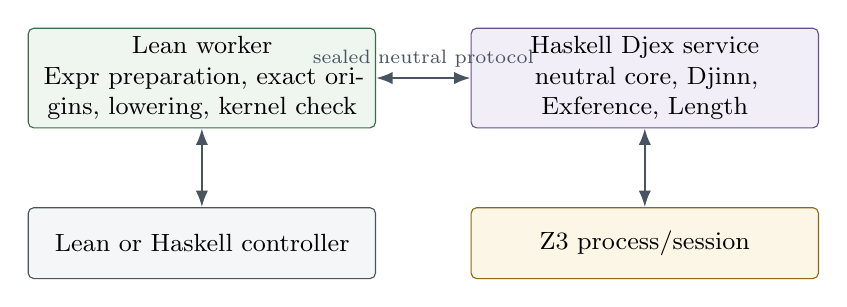
\begin{tikzpicture}[node distance=10mm and 12mm]
  \node[greenbox,text width=42mm] (lean) {Lean worker\\Expr preparation, exact origins, lowering, kernel check};
  \node[purplebox,right=of lean,text width=42mm] (haskell) {Haskell Djex service\\neutral core, Djinn, Exference, Length};
  \node[graybox,below=of lean,text width=42mm] (controller) {Lean or Haskell controller};
  \node[goldbox,below=of haskell,text width=42mm] (z3) {Z3 process/session};
  \draw[bothflow] (lean) -- node[above,note]{sealed neutral protocol} (haskell);
  \draw[bothflow] (controller) -- (lean);
  \draw[bothflow] (haskell) -- (z3);
\end{tikzpicture}
\caption{Best migration hybrid: Lean owns exact source identity and final trust; Haskell retains the current synthesis implementation behind a neutral protocol.}
\end{figure}

\subsection{Benefits}

\begin{itemize}
  \item removes generated Lean serializer source and Haskell S-expression parsing immediately;
  \item makes the final candidate an exact \code{Expr} and strengthens verification;
  \item preserves the mature Haskell search and semantic engines during differential development;
  \item cleanly separates project-toolchain-specific Meta code from a toolchain-neutral search process;
  \item makes the protocol a deliberate neutral IR rather than an accidental mix of Lean REPL and synthesis payloads;
  \item supports a future remote or sandboxed engine.
\end{itemize}

\subsection{Costs}

\begin{itemize}
  \item exact Lean origin handles cannot cross; the neutral problem must contain stable IDs and sufficient metadata;
  \item candidates and typed graphs must be serialized, preserving bounds and canonical identity;
  \item the worker must re-associate every returned ID with the exact current origin table;
  \item process overhead and protocol/versioning remain;
  \item semantic graph/certificate carriers that are currently opaque Haskell objects need a durable wire representation or must remain usable only inside the Haskell service;
  \item direct interactive inspection of search internals requires additional protocol messages.
\end{itemize}

\subsection{Permanent viability}

This is a respectable permanent architecture if toolchain-neutral search deployment is a priority. It is not the simplest Lean-only system. The boundary should be below Leant's exact origin and above Djex's checked request. Haskell must never return Lean text as the sole candidate; it returns a neutral generated term with exact neutral IDs and a checked-engine receipt. The Lean worker independently checks the neutral candidate and lowers it.

For Length, there are two choices:

\begin{enumerate}
  \item keep typed graph and Length entirely in the Haskell service; return only structured assessment views/receipts bound to a service candidate token;
  \item define a durable associated-graph/certificate wire schema and let Lean run Length.
\end{enumerate}

The first is safer initially. The second is essentially the beginning of porting the semantic layer.

\section{Hybrid 2: Lean Djinn, Haskell Exference plus typed semantics}

\subsection{Shape}

The shared neutral core is defined in a versioned protocol or implemented on both sides. Lean runs Djinn and its checker, while Haskell runs Exference, typed graph/certificate association, Length, and Z3. Leant merges candidate views in Lean and kernel-checks all results.

\subsection{Why this split is coherent}

Djinn and Exference already have deliberately separate centers and evidence semantics. Djinn does not currently provide the complete typed graph authority required by Length; Exference does. Porting Djinn first therefore creates a natural temporary portfolio:

\begin{itemize}
  \item Lean Djinn can establish the new fragment/compiler/checker/lowering path;
  \item Haskell Exference preserves ranked provider-oriented synthesis and Length;
  \item combined mode remains useful;
  \item Exference's semantic authority stays in one language/process rather than being torn apart.
\end{itemize}

\subsection{Risks}

\begin{itemize}
  \item the same neutral type, provider assignment, and generated-term semantics exist in two implementations;
  \item differential equivalence becomes a protocol requirement;
  \item candidate merge/deduplication must not transfer Haskell semantic authority to a Lean Djinn view;
  \item negative evidence from Lean Djinn depends on the Lean compiler ledger, while Haskell Exference preparation may project the problem differently unless the shared prepared problem is serialized once;
  \item maintaining both implementations indefinitely has real semantic-drift cost even when implementation volume is ignored.
\end{itemize}

\subsection{Judgment}

\textbf{Excellent staged architecture; acceptable permanent portfolio only if implementation diversity is deliberately desired.} If retained permanently, define the neutral problem and generated candidate wire schemas as first-class specifications with conformance suites.

\section{Hybrid 3: Lean synthesis engines inside a project worker, Haskell controller}

\subsection{Shape}

Port all semantic code to Lean, but retain Leant's Haskell executable as the terminal controller. It starts the project-local Lean worker, sends commands, presents candidates, maintains durable history, and handles recovery. The worker runs preparation, Djinn, Exference, Length, Z3, lowering, and kernel checks.

\subsection{Benefits}

\begin{itemize}
  \item preserves Haskeline and the mature controller/process code;
  \item gains nearly all semantic benefits of the rewrite;
  \item keeps the globally installed frontend independent of target Lean versions;
  \item provides a narrow controller protocol and straightforward recovery;
  \item avoids spending design attention on terminal UI while porting semantic code.
\end{itemize}

\subsection{Costs}

\begin{itemize}
  \item Haskell remains a runtime/build dependency for standalone use;
  \item some session/replay logic is split between controller and worker;
  \item native tactic/editor users do not need the Haskell controller, producing two frontend stacks;
  \item the project has not literally rewritten both libraries entirely in Lean.
\end{itemize}

\subsection{Judgment}

\textbf{Strong partial steady state.} If the goal is semantic simplification rather than language purity, this option captures most benefits at low architectural risk. Under the stated question, where a full Lean rewrite is being evaluated and effort is neutral, it is better as an intermediate state than the final target.

\section{Hybrid 4: Haskell search core embedded through FFI in a Lean process}

A Lean worker could call a Haskell shared library through C ABI. This avoids a process protocol but creates a difficult runtime composition: GHC RTS initialization, callback/threading rules, memory ownership, exceptions, cancellation, and crash containment all cross one process. It also makes target-toolchain builds depend on Haskell artifacts and weakens the independent worker boundary.

\textbf{Judgment: not recommended.} A subprocess protocol is safer, more debuggable, and semantically clearer. The data already needs a bounded neutral representation; making it an FFI ABI adds fragility without removing the conceptual boundary.

\section{Hybrid 5: Lean Djex engine, Haskell Leant synthesis bridge}

This inverted split keeps the current Haskell fragment/parser/renderer machinery but replaces Djex with a Lean service. It preserves the most accidental representation crossings while adding another language/process boundary. The Haskell frontend would still generate Lean serializer source, parse fragments, translate them into a wire problem, receive neutral candidates, render Lean text, and ask Lean to elaborate them.

\textbf{Judgment: technically feasible but architecturally poor.} It gains some proof formalization in the engine while missing the largest simplification---direct source identity and direct expression lowering. It is only sensible as a narrow test harness during engine development.

\section{Hybrid 6: Lean search/checking, Haskell Length/Z3 service}

A generic semantic service can receive an associated typed graph plus provider summaries and a contract, then return sealed assessment views. The difficulty is that associated graph authority is deliberately nonreconstructible from a bare graph and independent certificate table. A wire format must itself become an authority-bearing certificate checked by the service.

If Exference moves to Lean but Length remains Haskell, either:

\begin{itemize}
  \item Lean emits a complete typed graph/certificate association proof object that Haskell validates and reseals; or
  \item Haskell trusts Lean's graph serialization as an input authority.
\end{itemize}

The first is possible but substantial; the second weakens the current trust model. Furthermore, candidate-specific provider/session associations must cross.

\textbf{Judgment: inadvisable as a permanent split.} Move Exference's typed graph and Length together. A temporary service can be used for differential comparison, but not as the preferred authority boundary.

\section{Hybrid 7: Lean semantic system plus C platform shim}

This is the recommended final ``hybrid,'' although it is not a Haskell/Lean split. All project semantics are Lean. A small C component implements descriptor-bound process launch or line-editing primitives. C returns no synthesis, proof, or semantic verdict.

\textbf{Judgment: recommended.} It respects the actual abstraction boundary: operating-system mechanism below, checked policy and semantics above.

\section{Hybrid comparison}

\begin{longtable}{@{}L{0.21\textwidth}C{0.11\textwidth}C{0.13\textwidth}C{0.13\textwidth}L{0.27\textwidth}@{}}
\toprule
\textbf{Hybrid} & \textbf{Boundary quality} & \textbf{Lean benefit captured} & \textbf{Permanent fit} & \textbf{Recommendation} \\
\midrule
\endhead
Lean Meta/verify + Haskell Djex service & High & High & Good & Best first migration boundary; acceptable service architecture \\
Lean Djinn + Haskell Exference/Length & High & Medium--high & Conditional & Excellent staged portfolio; keep Exference and semantics together \\
Lean semantic worker + Haskell controller & Very high & Very high & Very good & Strong partial end state; later port controller if desired \\
Haskell library via FFI & Low & Medium & Poor & Avoid; use subprocess \\
Lean Djex + Haskell synthesis bridge & Low & Low--medium & Poor & Misses main simplification \\
Lean Exference + Haskell Length service & Medium--low & High & Poor & Splits opaque typed authority; avoid permanently \\
Lean + C platform shim & Very high & Full & Excellent & Recommended final architecture \\
\bottomrule
\end{longtable}

\section{Protocol requirements for any Haskell/Lean split}

If Haskell remains, the protocol should satisfy all of the following:

\begin{itemize}
  \item versioned schemas with explicit maximum sizes and recursion depths;
  \item exact neutral IDs scoped to one prepared problem, never raw Lean names as sole authority;
  \item alpha-normal/canonical encoding for types and generated terms;
  \item separate progress, truncation, evidence, and candidate fields;
  \item no raw lazy lists; chunked cursor requests with continuation tokens;
  \item environment/problem fingerprint in every continuation and candidate token;
  \item exact provider assignment vectors with kinds and source IDs;
  \item candidate checker version and graph-availability reason;
  \item no interpretation of raw solver statuses by the other side;
  \item bounded diagnostics and stderr; cancellation and worker poisoning rules;
  \item differential round-trip tests generated from both implementations.
\end{itemize}

A binary codec may be more efficient, but canonical JSON or CBOR is adequate initially. The semantic schema matters more than the encoding. The protocol should not serialize Haskell or Lean implementation records wholesale.

\section{Best partial-rewrite recommendation}

If a complete rewrite is postponed or deliberately avoided, the best target is:

\begin{quote}
\textbf{A Haskell controller and Haskell Djex service initially, wrapped by a project-local Lean worker that owns direct fragment preparation, exact origin tables, lowering, and kernel verification; then port Djinn; finally port Exference and its typed semantic/Length stack together.}
\end{quote}

If only one permanent Haskell component is retained, retain the controller rather than the semantic core. UI/process orchestration gains the least from Lean and has the weakest trust role. Search, checking, candidate identity, and semantic replay gain the most.

\begin{summarybox}
Partial rewrites are feasible, but boundaries matter more than percentages. The clean Haskell/Lean seam is a bounded neutral synthesis protocol. The unclean seam is inside an opaque typed-candidate/graph/Length association. Port exact Lean preparation early; port Djinn first; keep Exference and typed semantics together; retain Haskell longest at the controller edge, not in the trust-bearing center.
\end{summarybox}

\chapter{Migration and validation plan}\label{ch:migration}

The ordering below is based on semantic dependency and risk isolation, not cost. Each phase should produce a usable system and a differential oracle before the next authority moves.

\section{Phase 0: freeze observable semantics}

Before porting, define a machine-readable corpus from the current pinned revisions. For each test case, record:

\begin{itemize}
  \item source target and project/import fixture;
  \item prepared fragment and completeness reasons;
  \item provider inventory, exact assignments, and ground class facts;
  \item engine options and global budgets;
  \item normalized search events and completion evidence;
  \item neutral candidate ASTs before rendering;
  \item displayed variants and kernel-verification result;
  \item typed graph availability, canonical fingerprint, and certificate summary;
  \item Length sealing/refusal, canonical query fingerprint, replay result, and live observation transcript;
  \item session commands, worker failure injections, and reconstructed state.
\end{itemize}

Do not define the oracle as exact human-readable diagnostics or raw internal allocation IDs. Preserve exact candidate ordering where it is part of UX, but normalize IDs and paths that are intentionally incidental.

Add adversarial fixtures for cyclic/overlong protocol shapes, malformed S-expressions/JSON, stale environment IDs, process death at every transaction point, partial snapshot publication, unexpected Z3 output, huge numerals, repeated timeouts, and candidate tokens from prior generations.

\section{Phase 1: Lean direct fragment and origin preparation}

Implement \filepath{Leant/Meta/Fragment} and \filepath{Leant/Meta/Providers} in a project-local Lean worker. Keep the Haskell engine. The worker serializes a neutral problem equivalent to the current Haskell translation.

Acceptance gates:

\begin{itemize}
  \item fragment canonical equality on the corpus, modulo deliberate schema improvements;
  \item identical safe/unsafe/incomplete classifications;
  \item exact provider and assignment vectors;
  \item no generated Lean serializer source in the new path;
  \item bounded traversal and cancellation tests;
  \item project matrix across supported Lean versions.
\end{itemize}

Run both preparers in shadow mode where possible and report structural diffs without affecting results.

\section{Phase 2: Lean lowerer and kernel verifier}

Define the neutral generated AST codec and implement exact Lean lowering. Initially consume current Haskell Djex candidates. Add the scratch-environment kernel checker and optional display round-trip.

Acceptance gates:

\begin{itemize}
  \item every current accepted candidate lowers and kernel-checks;
  \item every known rejected/malformed candidate remains rejected;
  \item no unresolved term or universe metavariables survive;
  \item local scope abstraction is correct for dependent contexts;
  \item displayed text re-elaborates where the current UI promises copy-paste terms;
  \item renderer failure cannot invalidate or relabel a semantically valid \code{Expr};
  \item exact source names, implicit arguments, and constructor identities survive.
\end{itemize}

At the end of this phase, Lean owns both ends of the synthesis pipeline even though Haskell still searches the neutral middle.

\section{Phase 3: Lean shared synthesis core}

Port names, kinds, types, constraints, declarations, environments, queries, generated terms, progress, diagnostics, and provider evidence. Define canonical wire encodings and run Haskell/Lean smart constructors against the same generated cases.

Acceptance gates:

\begin{itemize}
  \item alpha-equivalence/substitution/kind tests agree;
  \item all checked constructors enforce the same finite bounds;
  \item environment construction has transactional indexes and deterministic diagnostics;
  \item canonical fingerprints are cross-implementation identical or version-bumped deliberately;
  \item Haskell frontends are not ported into this core.
\end{itemize}

Property generators should include nested foralls, opaque atoms with free variables, higher-kinded applications, tuples, constraints, aliases, recursive family references, and exact provider vectors.

\section{Phase 4: Lean Djinn}

Port the formula compiler, plan family, LJT cursor, normalization, proof checker, lowering, and evidence. Run Lean and Haskell Djinn side by side over the same prepared neutral problem.

Acceptance gates:

\begin{itemize}
  \item every Lean-emitted proof passes the Lean checker and every lowered term passes the kernel;
  \item normalized candidate sets and order agree under deterministic policies;
  \item global budgets/cutoffs and one-extra-proof truncation witnesses agree;
  \item complete/exhausted versus undecided classifications agree;
  \item self-reference-only diagnostic behavior agrees;
  \item a proved checker-soundness theorem covers the reified calculus before Djinn is considered authoritative for positive candidates.
\end{itemize}

The Haskell Djinn can remain as a shadow oracle after cutover. Divergence is categorized as bug, intended ordering difference, or deliberate language-fragment change.

\section{Phase 5: Lean Exference checker and typed graph}

Port the neutral expression checker before the scheduler. Feed it Haskell-generated candidate ASTs and origin annotations. Then port graph sealing, fingerprints, certificate tables, and associations.

Acceptance gates:

\begin{itemize}
  \item checker accept/reject and residual constraints agree;
  \item graph availability reasons agree;
  \item canonical graph fingerprints agree for reindexings and current candidates;
  \item certificate-bearing graphs cannot be authorized from bare projections;
  \item lossy equality/deduplication tests cannot discard association authority;
  \item Lean lowering/kernel check remains a separate final gate.
\end{itemize}

This phase establishes the authority consumed by Length before search performance becomes a variable.

\section{Phase 6: Lean Exference search}

Port unification, scope forest, node builder, expansion families, score, queue, scheduler cursor, and exact progress. Compare normalized traces.

Acceptance gates:

\begin{itemize}
  \item top-\(k\) candidate sets/order match representative fixtures;
  \item exact queue/depth prune counts and completion reasons match;
  \item search never promotes exhaustion to refutation;
  \item cancellation latency and worker-kill recovery meet the controller contract;
  \item memory/time benchmarks meet explicit thresholds;
  \item candidate quality does not regress merely because data-structure tie-breaking changed;
  \item independent checker rejects injected malformed solved nodes.
\end{itemize}

Only after this phase should the Haskell Exference runtime be removed from the normal path.

\section{Phase 7: Lean Length semantics and pure replay}

Port checked contracts, provider summaries, session/problem sealing, symbolic interpreter, concrete evaluators, applicable-domain validators, typed QF\_LIA, canonical query rendering, and offline replay. Keep live Z3 in Haskell or as an external transcript producer initially.

Acceptance gates:

\begin{itemize}
  \item identical seal/refusal precedence and policy/schema fingerprints;
  \item identical canonical SMT bytes for version-preserving paths;
  \item identical replay/counterexample receipts on recorded observations;
  \item finite-domain validators agree on applicability, coverage count, counterexample, and established result;
  \item no bare graph or names-only law list can construct a problem;
  \item interpreter/replay soundness theorems cover the supported graph rules.
\end{itemize}

\section{Phase 8: Lean Z3 protocol and process owner}

Port incremental parsing, causal stream, deadlines, sessions, readiness, execution-policy fingerprints, and ordinary process spawn. Bind the C descriptor launcher last.

Acceptance gates:

\begin{itemize}
  \item recorded transcripts produce identical bounded observations;
  \item fake-Z3 fixtures cover every framing, timeout, stderr, exit, and stale-response case;
  \item a poisoned session is never reused;
  \item worker teardown closes handles and reaps processes on Windows and POSIX;
  \item ordinary and hardened launch policies have distinct exact fingerprints;
  \item C FFI failure paths leak no descriptors and expose no raw handles;
  \item raw \code{sat}/\code{unsat}/\code{unknown} remains nonauthoritative without replay/certificate.
\end{itemize}

\section{Phase 9: Lean session worker and controller}

Move session replay, undo, snapshots, and replacement into the Lean worker/controller architecture. The Haskell controller can remain until the Lean controller reaches feature parity.

Acceptance gates:

\begin{itemize}
  \item every acknowledged command survives worker replacement;
  \item timed-out/ambiguous commands are not silently retried;
  \item reset/load/reload can bypass bad replay history;
  \item snapshots validate exact artifacts and tooling ABI;
  \item candidate tokens and environment capabilities fail after generation/worker replacement;
  \item generated \code{itN} names never collide across replay, snapshots, or gaps;
  \item terminal/UI behavior is tested separately from semantic correctness.
\end{itemize}

\section{Phase 10: native tactic and editor clients}

Expose \code{leant}, \code{leant?}, and structured commands over the same worker/core. Small searches may run in process; expensive work delegates. Add widgets or protocol clients without changing semantic authority.

\section{Differential architecture}

During migration, the old and new implementations should be executable under one harness:

\begin{lstlisting}[language=Leanish]
structure NormalizedRun where
  preparedFingerprint : Fingerprint
  events              : Array NormalizedSearchEvent
  candidates          : Array CandidateFingerprint
  completion          : Completion
  semanticAssessments : Array AssessmentFingerprint

inductive DifferentialResult where
  | equal
  | expectedDifference (reason : DifferencePolicy)
  | regression (diff : StructuredDiff)
\end{lstlisting}

The harness should support four comparisons:

\begin{itemize}
  \item Haskell versus Lean at the same layer;
  \item direct Lean preparation versus legacy serializer/parser preparation;
  \item neutral checker versus final kernel result;
  \item live Z3 execution versus replay of the captured observation.
\end{itemize}

\section{Testing layers}

\subsection{Unit and property testing}

Generate well-formed and malformed neutral types, substitutions, scopes, graphs, contracts, and SMT responses. Check round trips, alpha invariance, bounds, and checker properties. Lean's theorem layer can prove universal properties for small pure cores; executable generators find integration mistakes and performance pathologies.

\subsection{Model checking small search spaces}

For bounded tiny formula/type universes, enumerate all formulas/contexts and compare:

\begin{itemize}
  \item declarative derivability;
  \item checker acceptance;
  \item unbounded search result;
  \item normalization/lowering;
  \item kernel acceptance of the interpreted candidate.
\end{itemize}

This is particularly useful before a full LJT completeness proof.

\subsection{Fault injection}

Inject faults at every IO boundary: short writes, split UTF-8/SMT tokens, stderr floods, child exit before readiness, kill during model output, clock expiry between transaction phases, snapshot rename failure, disk-full publication, controller disconnect, and worker crash after commit but before acknowledgement.

\subsection{Performance and quality benchmarks}

Maintain fixed corpora for structural, library/provider, rank-N, recursive family, and semantic ranking cases. Record:

\begin{itemize}
  \item time to first checked candidate;
  \item time/allocations for first \(k\);
  \item peak worker memory;
  \item candidate quality/order metrics;
  \item queue/prune statistics;
  \item kernel-check and delaboration overhead;
  \item Z3 session reuse and replay-hit rates;
  \item restart/replay latency.
\end{itemize}

A faster engine that changes the top result from useful to pathological is a regression. A slower debug/proof build may be acceptable if optimized native deployment meets the explicit target.

\begin{summarybox}
The migration should move exact Lean preparation and verification first, then the neutral core, Djinn, Exference checker/graph, Exference search, Length, Z3 runtime, and finally the controller. This ordering keeps an executable oracle at every step and never splits Exference's typed semantic authority in the final state.
\end{summarybox}

\chapter[Trust model and formal-verification roadmap]{Trust model and formal-verification\\roadmap}\label{ch:trust}

\section{The trusted computing base after the rewrite}

A semantic full rewrite does not make the trusted base equal to ``the Lean kernel.'' Different result classes depend on different components.

\begin{figure}[H]
\centering
\resizebox{0.95\textwidth}{!}{%
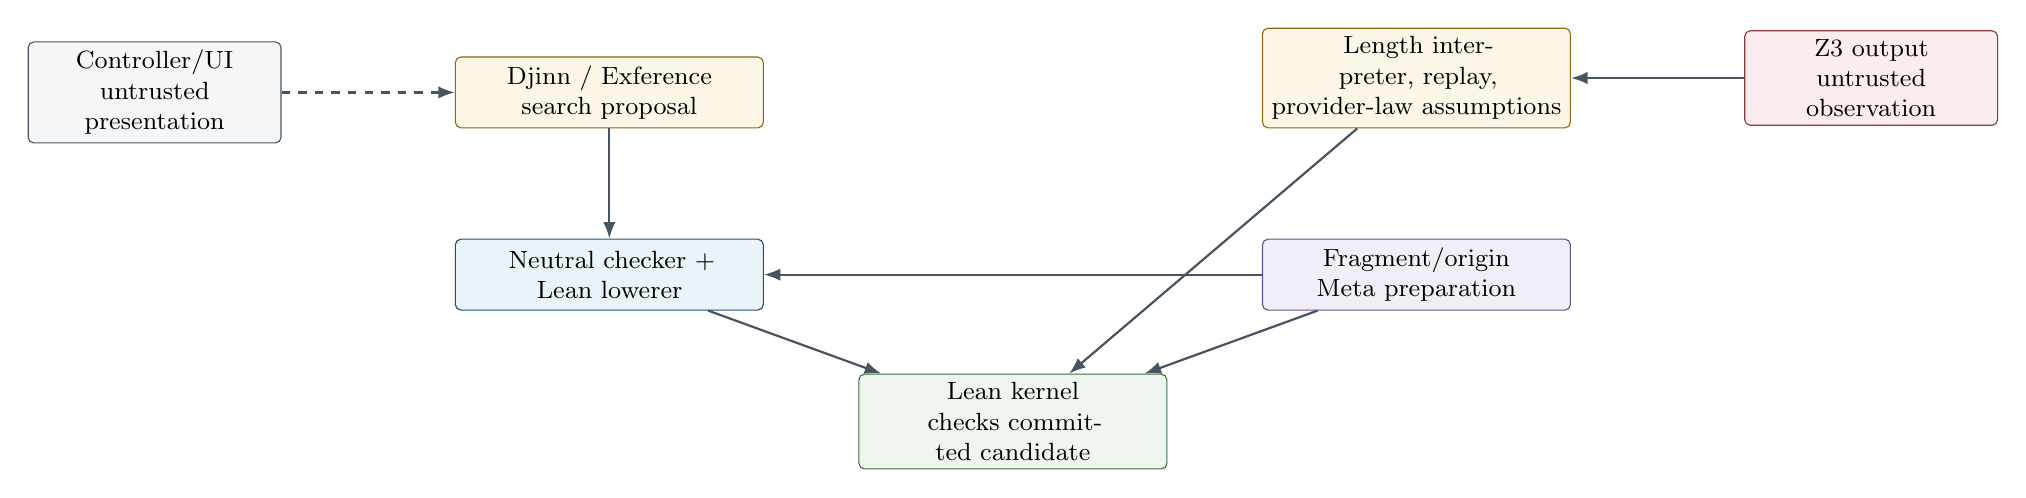
\begin{tikzpicture}[node distance=8mm and 12mm]
  \node[greenbox,text width=37mm] (kernel) {Lean kernel\\checks committed candidate};
  \node[box,above left=of kernel,text width=37mm] (lower) {Neutral checker +\\Lean lowerer};
  \node[purplebox,above right=of kernel,text width=37mm] (meta) {Fragment/origin\\Meta preparation};
  \node[goldbox,above=14mm of lower,text width=37mm] (search) {Djinn / Exference\\search proposal};
  \node[goldbox,above=14mm of meta,text width=37mm] (semantic) {Length interpreter, replay,\\provider-law assumptions};
  \node[redbox,right=22mm of semantic,text width=30mm] (z3) {Z3 output\\untrusted observation};
  \node[graybox,left=22mm of search,text width=30mm] (controller) {Controller/UI\\untrusted presentation};

  \draw[flow] (search) -- (lower);
  \draw[flow] (meta) -- (lower);
  \draw[flow] (lower) -- (kernel);
  \draw[flow] (meta) -- (kernel);
  \draw[flow] (semantic) -- (kernel);
  \draw[flow] (z3) -- (semantic);
  \draw[dashflow] (controller) -- (search);
\end{tikzpicture}}
\caption{Trust flows. Positive type correctness terminates at the kernel. Negative and behavioral claims require additional checked chains and remain qualified.}
\end{figure}

For a \term{positive candidate}, the required trusted components are Lean's kernel and the exact expected target/environment. Search, neutral checking, and lowering may be buggy, but a kernel-checked declaration still has the claimed Lean type (subject to the usual Lean axioms/options and no kernel-skip mode).

For a \term{Djinn negative conclusion}, the trusted chain includes:

\begin{itemize}
  \item correctness/adequacy of fragment projection;
  \item correctness and completeness classification of formula compilation/plans;
  \item completeness of the selected unbudgeted LJT procedure for the admitted formula;
  \item truthful exhaustion/progress accounting;
  \item the metatheoretic implication from formula unprovability to source uninhabitability.
\end{itemize}

For a \term{Length counterexample}, the chain includes:

\begin{itemize}
  \item exact candidate/graph/certificate association;
  \item correctness of provider-law selection and any ground discharge;
  \item symbolic interpreter and concrete replay;
  \item contract semantics and role policy;
  \item the stated provider summaries as assumptions;
  \item not Z3's raw verdict, because model values are independently replayed.
\end{itemize}

For an \term{applicable-domain established} result, the finite coverage extractor/enumerator/evaluator replaces Z3 but must itself be sound and complete for the recognized precondition grammar.

\section{Proof tiers}

A practical roadmap distinguishes five tiers.

\subsection{Tier 1: boundary construction invariants}

Use private constructors and executable checks for:

\begin{itemize}
  \item finite bounds and index validity;
  \item environment/index coherence;
  \item closed substitutions and provider vectors;
  \item scope forests and graph references;
  \item policy/schema consistency;
  \item process/session state transitions.
\end{itemize}

These need not all carry propositions at runtime. Their guarantee is module abstraction plus tests.

\subsection{Tier 2: total checker soundness}

Prove total checkers sound against declarative judgments:

\begin{itemize}
  \item Djinn proof checker;
  \item neutral generated-term scope checker;
  \item Exference expression checker;
  \item typed graph well-formedness checker;
  \item QF\_LIA typed AST checker/parser;
  \item contract and provider-summary checker.
\end{itemize}

This tier removes search and parser bugs from positive evidence.

\subsection{Tier 3: transformation preservation}

Prove selected pure transformations preserve meaning:

\begin{itemize}
  \item alpha normalization and substitution;
  \item proof-term normalization;
  \item proof-to-neutral-term lowering;
  \item neutral-term simplification;
  \item graph reindexing/canonical encoding;
  \item Length symbolic interpretation rules;
  \item arithmetic canonicalization and model replay.
\end{itemize}

The final Lean kernel check remains valuable even after these proofs because the origin mapping and Meta lowering sit outside the reified theorem.

\subsection{Tier 4: decision completeness}

Prove completeness/termination for a sharply delimited unbounded Djinn calculus and finite-domain validators. Keep heuristic Exference explicitly outside this tier.

The theorem should name the exact formula grammar and strategy. Budgeted cursors derive a weaker theorem: if they return exhausted without any truncation and the compilation is complete, then no proof exists in that grammar.

\subsection{Tier 5: source reflection}

Connect selected Lean targets to the reified fragment by a theorem or generated certificate. This is the most difficult tier. Possible restricted domains include:

\begin{itemize}
  \item proposition-valued formulas over exact opaque proposition constants;
  \item nondependent arrows/products/sums with exact constructors;
  \item a library of supported finite nonindexed inductives with generated reflection lemmas;
  \item explicit provider theorems associating source constants with neutral schemes/behavioral summaries.
\end{itemize}

For these domains, a no-proof result could potentially produce a kernel theorem or a checked reflection certificate. Outside them, retain the current audited completeness ledger rather than overstating proof strength.

\section{Can Djinn produce a Lean proof of uninhabitability?}

Not in general merely because proof search found no inhabitant. For a target type \(T\), a kernel theorem of uninhabitability is a term of \code{T -> False}, \code{Not (Nonempty T)}, or an \code{IsEmpty T} instance. Intuitionistic nonderivability of \(T\) from an empty context is a metatheoretic statement; it is not automatically an object-language proof of \(\neg T\).

For finite decidable reified formula models, one can prove a theorem that the decision procedure's negative result implies no term of the interpreted type. To turn that into \code{T -> False}, the interpretation must provide an eliminator or equivalence strong enough to construct the negation. For arbitrary type atoms, this may require classical reasoning or a semantic model not internalized as a term.

The rewrite should therefore keep at least these user-facing labels distinct:

\begin{itemize}
  \item \term{kernel-checked inhabitant};
  \item \term{verified no proof in the reified calculus};
  \item \term{source uninhabitability established under complete projection};
  \item \term{kernel theorem of uninhabitability} (only when an actual theorem is produced).
\end{itemize}

\section{Verifying the Lean fragment builder}

The fragment builder runs in \code{MetaM} over \code{Expr} and environment metadata. Proving the entire Lean elaborator/environment implementation correct is unrealistic. More achievable approaches are:

\begin{enumerate}
  \item \term{Proof by final positive check}: for candidates, rely on the kernel and do not need a fragment-builder soundness theorem.
  \item \term{Certificate-producing projection}: the builder emits a reified derivation explaining each structural correspondence; a small checker validates the derivation against the source expression.
  \item \term{Generated equivalence term}: for selected structural forms, build Lean terms witnessing an equivalence or pair of translations between the source type and an interpreted fragment.
  \item \term{Restricted reflection elaborator}: support only syntactic forms whose exact \code{Expr} shape is recognized without unfolding; negative evidence is enabled only there.
  \item \term{Audit ledger}: for broader practical synthesis, continue current explicit safety/incompleteness reasons without claiming kernel-certified reflection.
\end{enumerate}

The recommended system uses all five at different strengths.

\section{Provider summaries}

Behavioral provider summaries are an explicit assumption unless they are accompanied by Lean theorems. A Lean rewrite can improve this substantially:

\begin{itemize}
  \item a provider summary declaration can name a theorem proving the Length law;
  \item preparation kernel-checks the theorem and extracts a supported law certificate;
  \item the semantic used-law basis retains the theorem's exact name/environment identity;
  \item a counterexample receipt can state that it is unconditional with respect to that provider because the law was kernel-certified;
  \item summaries without theorems remain user/configuration assumptions and are labeled accordingly.
\end{itemize}

This creates a continuum from assumed library specifications to fully checked provider laws without requiring Z3 proof checking.

\section{Solver certificates}

The current Length use is counterexample-oriented, so replaying model values is sufficient for \code{sat}-style evidence. An \code{unsat} result is intentionally not proof authority. If future features need solver-proved universal facts, prefer proof-producing formats and verified checkers where available. Z3 proof objects for the full relevant theory may be difficult to consume robustly; an alternative is to lower to a supported certificate dialect or use Lean-native arithmetic procedures for bounded/linear subgoals.

The rewrite should not make a universal Z3 proof checker a prerequisite. Keep the existing existential-counterexample architecture and add certificates only for concrete features that need them.

\section{Runtime code and logical consistency}

Search and IO code may use \code{partial} definitions, arrays, mutable references, tasks, FFI, and exceptions. This does not threaten Lean's logical consistency as long as runtime-computed terms are submitted to the kernel and unsafe values are not inserted through kernel-check-skipping APIs. Build and runtime options must ensure \code{debug.skipKernelTC} or equivalent bypasses are never active in production verification.

A separate environment checker can validate durable snapshot \code{.olean} artifacts if the threat model includes faulty metaprograms adding unchecked declarations. The normal worker should never use \code{addDeclWithoutChecking} for accepted candidates.

\begin{summarybox}
The rewrite enables a layered assurance story: executable opaque boundaries, proved checker soundness, proved pure transformations, selected completeness theorems, and restricted source reflection. Positive type correctness can be kernel-based immediately; negative and behavioral claims must continue to name their additional assumptions.
\end{summarybox}

\chapter{Risk register}\label{ch:risks}

The table below treats ``risk'' as a threat to semantic fidelity, operational quality, or long-term architecture. It deliberately does not list implementation volume as a negative factor.

\begin{longtable}{@{}L{0.21\textwidth}C{0.09\textwidth}C{0.09\textwidth}L{0.51\textwidth}@{}}
\toprule
\textbf{Risk} & \textbf{Likeli\-hood} & \textbf{Impact} & \textbf{Mitigation / acceptance condition} \\
\midrule
\endhead
Lean Meta API churn & High & Medium & Isolate \filepath{Leant/Meta}; compile worker with project toolchain; maintain version adapters and CI matrix; include API/toolchain in cache and snapshot keys. \\
Exference performance regression & Medium & High & Explicit normalized trace oracle; benchmark time-to-first/top-\(k\), memory, and candidate quality; choose queue/maps empirically; retain Haskell fallback until thresholds pass. \\
Candidate-order drift & High & Medium & Stable neutral tie breakers; canonical iteration order; compare normalized traces; classify intentional versus accidental differences. \\
Over-indexed dependent hot state & Medium & Medium--high & Keep proofs/checkers at boundaries; compact private runtime nodes; inspect generated code and compile time; benchmark proof-bearing variants. \\
Accidental dependence on Lean metavariable internals & Medium & High & Preserve neutral search IR; restrict MetaM to preparation/lowering/final elaboration; never serialize or fingerprint raw mvar state. \\
Kernel check accidentally bypassed & Low & Critical & Centralize checker; assert options; use synchronous \code{Kernel.Environment.addDecl}/checked \code{addDecl}; production test rejects malformed declarations; never expose unchecked add path. \\
Stale origin/candidate capability & Medium & High & Environment-generation and worker-session tokens in every authority; private constructors; invalidate all tokens after undo/replay/replacement. \\
Renderer view becomes authority again & Medium & High & Retain exact \code{Expr}/neutral candidate; display returns view only; acceptance uses token; optional text round-trip is secondary. \\
Negative evidence overstated & Medium & Critical & Typed completeness reasons; separate operational exhaustion, verified formula result, source conclusion, and kernel theorem; require all witnesses at promotion boundary. \\
Typed graph authority split across languages & Medium during migration & High & Move Exference checker/graph/Length together; if service split exists, retain opaque service token or complete checked wire certificate. \\
Z3 raw status trusted & Low if architecture preserved & Critical & All public evidence constructors require sealed problem and independent replay; raw parser types stay package-private/untrusted. \\
Z3 framing/deadline race & Medium & High & Causal transaction state, ordinals, absolute deadlines, kill on ambiguity, fake worker fault matrix, no session reuse after error. \\
C FFI resource leak/ABI drift & Medium & High & Tiny borrowed/owned API; exhaustive failure cleanup; per-platform tests/sanitizers; versioned shim; ordinary spawn fallback as a distinct policy. \\
Controller/worker version mismatch & Medium & Medium & Capability handshake; protocol negotiation; fail before imports; cache key contains both versions. \\
Cross-toolchain artifact loading & Medium & Critical & Never load project modules in global controller; build project-local worker; reject incompatible \code{.olean}/snapshot family. \\
Async kernel check not awaited & Medium & High & Use synchronous check for scratch verification or explicitly await environment checked task before acknowledgement; tests inject delayed failure. \\
Worker crash after commit before acknowledgement & Low--medium & Medium & Controller records only acknowledged history; reconstruct from last commit; no token retry; generated-name scan prevents collisions. \\
Snapshot partial publication & Low--medium & High & Preserve temporary siblings, exact sidecar, backup/restore, streaming fingerprints, Windows rename tests. \\
Search cancellation too cooperative & Medium & Medium--high & Explicit checks in cursor steps; hard controller deadline kills worker; no shared durable state inside worker. \\
Protocol denial of service & Medium & High & Byte/depth/width/count limits before allocation/traversal; incremental parser; bounded diagnostics; request quotas. \\
Formal proof gives false confidence outside theorem domain & Medium & High & Publish exact theorem assumptions/grammar; keep runtime checks and kernel verification; label unverified Meta/FFI/solver boundaries. \\
Provider law misassociation & Medium & High & Exact theorem/constant identity, environment generation, checked provider binding, used-law derivation from occurrences, no names-only lookup. \\
Lean controller terminal UX regression & Medium & Low--medium & Retain Haskell controller temporarily; bind mature line editor; support editor/TUI clients over protocol. \\
\bottomrule
\end{longtable}

\section{Risks that favor keeping Haskell temporarily}

Three risks specifically justify a staged hybrid even though they do not argue against the final rewrite:

\begin{enumerate}
  \item Exference performance and candidate-order parity are best assessed against a live Haskell oracle.
  \item The current typed graph/Length authority is intricate; moving its checker before its search reduces simultaneous uncertainty.
  \item The Haskell controller provides a stable UX while the Lean worker/toolchain/cache protocol matures.
\end{enumerate}

No risk requires retaining the Haskell semantic implementation permanently.

\section{Risks that favor retaining a process boundary permanently}

\begin{itemize}
  \item arbitrary project metaprograms and imports can crash or consume unbounded resources;
  \item cancellation in pure code is cooperative;
  \item Lean worker binaries and \code{.olean} files are toolchain-specific;
  \item FFI and Z3 process code have system-level failure modes;
  \item durable history should survive worker replacement;
  \item ambiguous in-flight command status is easier to resolve by reconstructing from acknowledged state.
\end{itemize}

These remain after Haskell is gone.

\chapter{Final recommendation}\label{ch:recommendation}

\section{Decision}

\begin{verdictbox}
\textbf{Proceed toward a full Lean 4 rewrite of all Lean-facing semantic components of Leant and Djex.}

Define the target as a Lean-native synthesis package and project-local worker, backed by a separate Lean controller for standalone use. Preserve independent neutral checkers, the final kernel declaration check, explicit completeness/evidence types, solver replay, and transactional process reconstruction. Retain a minimal C shim for descriptor-bound Z3 execution if that policy remains required. Do not port Haskell-source compatibility layers.
\end{verdictbox}

This recommendation is stronger than ``a partial rewrite is possible.'' Under the user's assumptions, a complete semantic rewrite is not only feasible; it removes a disproportionate amount of complexity that exists solely because Lean expressions and Lean candidates are temporarily represented in Haskell.

\section{Precise qualification}

The recommended end state is \emph{not}:

\begin{itemize}
  \item one monolithic Lean process;
  \item search directly over Lean metavariables;
  \item automatic trust in code because it is written in Lean;
  \item removal of the neutral fragment or completeness ledger;
  \item reliance on Z3 \code{unsat};
  \item text rendering as candidate authority;
  \item a literal port of historical Haskell frontends;
  \item forced removal of every non-Lean source file.
\end{itemize}

It is:

\begin{itemize}
  \item a Lean-oriented neutral synthesis IR with exact worker-local origin mappings;
  \item Djinn and Exference as separate checked engines over that IR;
  \item direct lowering to \code{Expr} and synchronous kernel verification;
  \item a typed graph/semantic system co-located with Exference's checker;
  \item pure semantic sealing/replay before optional live Z3;
  \item a project-toolchain-matched worker behind a bounded capability protocol;
  \item a controller whose failure/replay semantics remain close to current Leant;
  \item a narrow C boundary for OS primitives only.
\end{itemize}

\section{Recommended priority order}

Even with effort ignored, dependency order matters. The highest-value sequence is:

\begin{enumerate}
  \item direct Lean fragment/provider preparation;
  \item direct neutral-to-\code{Expr} lowering and kernel verification;
  \item shared neutral core;
  \item Djinn and its proved checker;
  \item Exference checker, typed graph, and certificate association;
  \item Exference scheduler/search;
  \item Length pure semantics and replay;
  \item Z3 protocol/session and C launch binding;
  \item worker session/replay/snapshots;
  \item Lean controller and native tactic/editor clients.
\end{enumerate}

This order maximizes early architectural benefit and keeps the current implementation available as an oracle.

\section{Best fallback if the full rewrite is rejected}

Retain Haskell at the outermost or most self-contained boundaries:

\begin{enumerate}
  \item best permanent partial state: Haskell controller, Lean project worker containing the full semantic system;
  \item best migration state: Lean preparation/lowering/verification around a Haskell Djex subprocess service;
  \item best split-engine state: Lean Djinn, Haskell Exference plus typed semantics/Length;
  \item avoid: Haskell/Lean FFI embedding or splitting Exference from its graph/Length authority.
\end{enumerate}

\section{Bottom-line answers to the user's questions}

\begin{longtable}{@{}L{0.39\textwidth}L{0.53\textwidth}@{}}
\toprule
\textbf{Question} & \textbf{Answer} \\
\midrule
\endhead
Is a complete rewrite in Lean 4 feasible? & \textbf{Yes.} All search, checking, semantic, protocol, session, and UI logic is implementable in Lean. Exact current hardened Z3 launch is best retained as a tiny C FFI primitive. \\
Is a complete rewrite advisable when work is not counted against it? & \textbf{Yes, for the Lean-only target.} It removes accidental representation crossings, gives exact source identity, improves integration and proof opportunities, and eliminates irrelevant Haskell frontends. \\
Should the result be one process? & \textbf{No, not as the default standalone design.} Preserve a project-local worker for toolchain and fault isolation. \\
Should Djex use Lean's raw \code{Expr}/metavariable state as its search language? & \textbf{No.} Keep a pure neutral IR and exact origin map; use MetaM at preparation/lowering boundaries. \\
Does rewriting in Lean make negative results formally proved? & \textbf{No, not automatically.} It enables proofs of checker/search/translation components, but source-projection completeness remains a separate obligation. \\
Does rewriting in Lean make Z3 trustworthy? & \textbf{No.} Preserve independent model replay and conditional provider-law semantics. \\
What is the best partial rewrite? & A Lean project worker for preparation/lowering/kernel checking with Haskell Djex as a subprocess, followed by Lean Djinn and then Exference+typed semantics together. \\
What Haskell component is most reasonable to retain longest? & The toolchain-neutral controller/UI, not the trust-bearing synthesis or semantic core. \\
\bottomrule
\end{longtable}

\begin{summarybox}
The language rewrite is feasible; the architecture rewrite is the real opportunity. Lean should own exact source identity, search checking, candidate lowering, semantic replay, and proof opportunities. Processes should continue to own failure isolation, and C should own only those OS primitives that genuinely sit below Lean's standard runtime.
\end{summarybox}


\appendix

\chapter{Source-to-rewrite map}\label{app:source-map}

This appendix maps the principal current source ownership boundaries to the recommended Lean-native structure. It is intentionally not a file-count estimate. Its purpose is to prevent two common rewrite errors: translating files one by one although their boundary is accidental, and merging modules whose separation currently encodes a real authority distinction.

\section{Leant source map}

\begin{longtable}{@{}L{0.27\textwidth}L{0.31\textwidth}L{0.34\textwidth}@{}}
\toprule
\textbf{Current source} & \textbf{Current responsibility} & \textbf{Recommended destination} \\
\midrule
\endhead
\lpath{src/Leant/Backend.hs} & Discovery and lifetime of the community REPL process; bounded JSON request cycle; timeout, stderr, and death handling. & Split between \code{Leant.Controller.WorkerProcess} and the project-local worker's protocol server. Preserve process death as loss of a lease, not corruption of durable session state. \\
\lpath{src/Leant/Synth/Fragment.hs} & Embedded Lean serializer source, S-expression parser, fragment datatype, provider wire shapes, and completeness analyses. & Replace the generated-source and parse portions by \code{Leant.Meta.Prepare}; move the pure fragment and ledger to \code{Djex.Source.Fragment}; retain only a versioned protocol codec for controller-to-worker communication. \\
\lpath{src/Leant/Synth/Engine.hs} & Translation to Djex declarations/types, engine lane construction, candidate merging, semantic sidecars, and exact-origin retention. & Decompose into \code{Djex.Source.Lower}, \code{Djex.Portfolio}, \code{Djex.Candidate}, and \code{Djex.Semantic.Origin}. The current large file contains several authorities which should become explicit Lean modules rather than one translated mega-module. \\
\lpath{src/Leant/Synth/Render.hs} & Conversion of generated terms and typed graphs to Lean source text using constructor, type, provider, and binder maps. & Split semantic lowering from presentation. \code{Djex.Lean.Lower} produces an \code{Expr}; \code{Djex.Lean.Present} pretty-prints the accepted expression or a deliberately reconstructed syntax term. Text ceases to be the acceptance key. \\
\lpath{src/Leant/Synth/Verification.hs} & Bounded callback verification and opaque acceptance receipts. & \code{Djex.Lean.Verify}: instantiate metavariables, reject holes and unauthorized axioms, create a scratch declaration, and synchronously invoke the kernel. Preserve opaque receipts and batch association. \\
\lpath{src/Leant/Synth/PostVerification.hs} & Generative occurrence handles and exact-permutation sealing after Lean acceptance. & \code{Djex.Candidate.AcceptedBatch}. Implement handles as nominal opaque values allocated by one batch owner; expose folds rather than detachable IDs. \\
\lpath{src/Leant/Synth/ProviderCache.hs} & Canonical provider-query keys and cache discipline. & \code{Leant.Meta.ProviderCache}, keyed by environment generation plus a structural query fingerprint. Never cache an \code{Expr}, \code{FVarId}, or declaration handle across worker generations. \\
\lpath{src/Leant/Session/Replay.hs} & Pure history-prefix and replay accumulation. & Port almost directly to \code{Leant.Session.Replay}; this is already language-neutral state-machine logic. Make acknowledgement ordinals and environment generations explicit types. \\
\lpath{src/Leant/Session/Snapshot.hs} & Snapshot artifact families, sidecar validation, fingerprints, publication, and ownership. & Divide into a toolchain-neutral controller manifest and worker-owned Lean environment artifacts. The synthesis ABI fingerprint should identify fragment, candidate, and protocol schemas rather than embedded serializer source text. \\
\lpath{src/Leant/Synth/Length/Handoff.hs} & Reassociation of accepted text with exact typed origin, family/provider resolution, and checked problem sealing. & \code{Djex.Semantic.Length.Handoff}, but associate the acceptance receipt directly with the candidate identity and accepted \code{Expr}. Remove the text-equality detour while preserving exact rendering-variant policy as presentation metadata when needed. \\
\lpath{src/Leant/Synth/Length/Ranking/Internal.hs} & Pure replay bank, applicable-domain validators, live-session orchestration, stable no-prune reordering, and fallback. & Split into \code{Djex.Semantic.Length.ReplayBank}, \code{ApplicableDomain}, \code{Ranking}, and \code{Live}. The pure validators should be individually theorem-friendly; live IO should consume their sealed results. \\
\lpath{src/Leant/Synth/Length/Configuration/File.hs} & One closed JSON grammar with exact object-field rejection and resource bounds; versionless since \code{4fa5c0a1}, just before the pin, when the numbered schema history was deleted rather than kept as fallbacks. & A Lean decoder with the same exact-field rejection and bounds. Keep the schema versionless but fingerprinted, so that history is never re-encoded as one ever-growing decoder function; the contract-only file adopted the same rule after the pin (\code{d4104c91}). \\
\lpath{src/Main.hs} & REPL UI, session state, proving, synthesis command orchestration, recovery, and presentation. & Split between \code{Leant.Controller}, \code{Leant.Worker}, and an optional \code{Leant.Command} executable. Native \code{leant} / \code{leant?} / \texttt{\#leant} clients call worker-local library APIs and need none of the standalone line editor. \\
\bottomrule
\end{longtable}

\section{Djex shared-foundation source map}

\begin{longtable}{@{}L{0.30\textwidth}L{0.30\textwidth}L{0.32\textwidth}@{}}
\toprule
\textbf{Current source family} & \textbf{Semantic ownership} & \textbf{Recommended Lean family} \\
\midrule
\endhead
\dpath{synthesis/src/Language/Haskell/Synthesis/Name.hs} and qualification modules & Validated names and namespace roles. & \code{Djex.Core.Name}. Use \code{Lean.Name} only for exact source globals; use distinct nominal types for engine constructors, locals, definitions, and classes. \\
\dpath{synthesis/src/Language/Haskell/Synthesis/Type.hs}, \filepath{Kind.hs}, \filepath{Constraint.hs}, and \filepath{TypeAtom.hs} & Neutral kinds/types, rigid/flexible identity, polytype atoms, substitution, and finite views. & \code{Djex.Core.Kind}, \code{Type}, \code{TypeAtom}, \code{Substitution}. Preserve opacity plus free-variable visibility for nested polytypes. \\
\dpath{synthesis/src/Language/Haskell/Synthesis/Declaration.hs} and \filepath{Environment.hs} & Checked declaration order and coherent indexes. & \code{Djex.Core.Declaration} and opaque \code{CheckedEnvironment}. Smart construction should remain transactional and separate from Lean's full environment. \\
\dpath{synthesis/src/Language/Haskell/Synthesis/Inventory.hs} & Search-oriented projection from checked declarations. & \code{Djex.Core.Inventory}; distinguish durable inventory from transient expansion views. \\
\dpath{synthesis/src/Language/Haskell/Synthesis/Generated.hs} & Shared generated-term language and scope checks. & \code{Djex.Term.Raw}, \code{Djex.Term.Checked}, and \code{Djex.Term.Simplify}. Prefer intrinsically distinguished local IDs but retain an independent scope checker rather than relying solely on constructors. \\
\dpath{synthesis/src/Language/Haskell/Synthesis/Query.hs}, \filepath{Search.hs}, and \filepath{Candidate.hs} & Requests, evidence, progress, truncation, batches, and backend details. & \code{Djex.Query}, \code{Djex.Search.Progress}, \code{Djex.Candidate}. Use indexed or opaque states to prevent a truncated stream from being reclassified as exhaustive. \\
\dpath{synthesis/src/Language/Haskell/Synthesis/TypedGenerated.hs} and internal certificate modules & Sealed typed graph, graph checking, certificate tables, and atomic associations. & \code{Djex.TypedGraph.*}. Move with Exference's checker and the Length handoff as one authority cluster. \\
\dpath{synthesis/src/Language/Haskell/Synthesis/TypedCandidate.hs} & Compatibility candidate plus optional graph/carrier state. & \code{Djex.TypedCandidate}. Avoid deriving equality that silently erases authority; provide explicit compatibility and authority-aware comparison views. \\
\dpath{synthesis/internal/Language/Haskell/Synthesis/Internal/ClassResolution.hs} & Checked ground instance/class resolution. & \code{Djex.ClassResolution}. This is a strong candidate for executable soundness lemmas because its domain is deliberately bounded and first-order. \\
\bottomrule
\end{longtable}

\section{Djinn source map}

\begin{longtable}{@{}L{0.29\textwidth}L{0.31\textwidth}L{0.32\textwidth}@{}}
\toprule
\textbf{Current source} & \textbf{Current responsibility} & \textbf{Recommended Lean destination} \\
\midrule
\endhead
\dpath{djinn/src-core/Djinn/Internal/LJTFormula.hs} & Formula, constructor descriptions, and proof-term language. & \code{Djex.Djinn.Formula} and \code{Proof}. Give formulas stable structural fingerprints independent of allocation IDs. \\
\dpath{djinn/src-core/Djinn/Internal/TypeFormula.hs} & Polarity-aware type-to-formula compiler, structural plans, and completeness ledger. & \code{Djex.Djinn.Compile}. Return a sealed \code{CompiledProblem} containing the formula, lowering map, exact premise evidence, and negative-evidence capability. \\
\dpath{djinn/src-core/Djinn/Internal/LJT.hs} & Lazy continuation-encoded LJT search and choice accounting. & \code{Djex.Djinn.Search.Cursor}; represent suspension explicitly. Preserve fair interleaving and shared budgets as observable state. \\
\dpath{djinn/src-core/Djinn/Internal/ProofCheck.hs} & Independent proof reconstruction. & \code{Djex.Djinn.Check}. Keep this small, total over finite proofs, and suitable for a theorem connecting accepted proof terms to formula semantics. \\
\dpath{djinn/src-core/Djinn/Internal/ProofToGenerated.hs} & Checked proof lowering to generated terms. & \code{Djex.Djinn.Lower}; require the exact \code{CompiledProblem} origin, not only a formula and proof. \\
\dpath{djinn/src-core/Djinn/Core.hs} & Plan portfolio, premise policy, search, evidence, deduplication, and ranking. & \code{Djex.Djinn.Engine} plus \code{Djex.Portfolio}. Separate logical evidence from presentation/ranking so a reordering cannot alter completeness classification. \\
\bottomrule
\end{longtable}

\section{Exference source map}

\begin{longtable}{@{}L{0.31\textwidth}L{0.29\textwidth}L{0.32\textwidth}@{}}
\toprule
\textbf{Current source family} & \textbf{Current responsibility} & \textbf{Recommended Lean destination} \\
\midrule
\endhead
\dpath{exference/src-core/Language/Haskell/Exference/Core/Unify.hs} & Scope-sensitive first-order/higher-kinded unification with opaque polytypes. & \code{Djex.Exference.Unify}; make namespace/origin tags part of the variable key and prove substitution preservation properties over checked finite types. \\
\dpath{exference/src-core/Language/Haskell/Exference/Core/Internal/ExferenceNode.hs} and builder & Complete partial-program state: holes, scopes, substitutions, givens, usage, expression, and freshness. & \code{Djex.Exference.Node}. Keep it immutable at the semantic layer; use local mutation only inside verified update functions or queue implementation. \\
\dpath{exference/src-core/Language/Haskell/Exference/Core/Internal/Exference.hs} & Priority scheduler, expansion, queue/depth pruning, result stream, and metrics. & \code{Djex.Exference.Search.Cursor}, \code{Expand}, and \code{Queue}. Explicitly return the cursor after each yielded candidate. \\
\dpath{exference/src-core/Language/Haskell/Exference/Core/Score.hs} & Heuristic scoring and ordering. & \code{Djex.Exference.Score}; use deterministic total ordering and version its feature vector if candidate order is externally compared. \\
\dpath{exference/src-core/Language/Haskell/Exference/Core/ExpressionCheck.hs} and internal checker & Independent bidirectional reconstruction and exact residual-constraint check. & \code{Djex.Exference.Check}; produce the typed graph and certificate association in the same successful transaction. \\
\dpath{exference/src-core/Language/Haskell/Djex/Exference.hs} and internal request/session owners & Checked neutral-to-engine projection and sealed run authority. & \code{Djex.Exference.Session}, \code{Request}, and \code{Engine}. Preserve the exact inventory, provider assignments, source-name map, and policy in candidate origin. \\
\bottomrule
\end{longtable}

\section{Semantic and Z3 source map}

\begin{longtable}{@{}L{0.31\textwidth}L{0.29\textwidth}L{0.32\textwidth}@{}}
\toprule
\textbf{Current source family} & \textbf{Current responsibility} & \textbf{Recommended destination} \\
\midrule
\endhead
\dpath{synthesis/src/Language/Haskell/Synthesis/Semantic/Problem.hs} and \filepath{Observation.hs} & Generic problem identity and status-indexed observations. & \code{Djex.Semantic.Problem} and \code{Observation}. Encode status-dependent projections with indexed inductives or opaque eliminators, not optional fields. \\
\dpath{synthesis/src/Language/Haskell/Synthesis/Semantic/Length.hs} and internal implementation & Versioned Length vocabulary, symbolic expressions/formulas, provider laws, and limits. & \code{Djex.Semantic.Length.Syntax}, \code{Contract}, \code{Provider}, and \code{Limits}. This is pure and especially suitable for theorem-backed constructors. \\
\dpath{synthesis/src/Language/Haskell/Synthesis/Semantic/Length/Problem.hs} & Checked session, contract, candidate interpretation, and complete problem identity. & \code{Djex.Semantic.Length.Problem}. Keep session-owned sealing so independently chosen contract and candidate policies cannot be recombined. \\
\dpath{synthesis/src/Language/Haskell/Synthesis/Semantic/Length/Evaluate.hs} & Bounded concrete replay and counterexample construction. & \code{Djex.Semantic.Length.Evaluate}. Prove that a returned counterexample falsifies the normalized contract under the recorded provider assumptions. \\
\dpath{synthesis/src/Language/Haskell/Synthesis/Semantic/Length/SMTLib.hs} and QF\_LIA internals & Typed linear arithmetic, canonical bytes, fingerprints, model bindings, and replay. & \code{Djex.SMT.QFLIA}, \code{Render}, and \code{Replay}. Keep the typed plan as the authority and bytes as a projection. \\
\dpath{synthesis/internal/Language/Haskell/Synthesis/Internal/SMTLib/Response.hs} and causal stream modules & Bounded lexer/parser, framing, transaction boundaries, and response classification. & \code{Djex.SMT.Response} and \code{Transport.Causal}. Keep byte, token, node, depth, and numeral limits in one process-owned policy. \\
\dpath{synthesis/internal/Language/Haskell/Synthesis/Internal/SMTLib/Z3/Execution.hs} & Complete launch profile and identity. & \code{Djex.Z3.ExecutionPolicy}; pure validation/fingerprinting in Lean. \\
\dpath{synthesis/internal/Language/Haskell/Synthesis/Internal/SMTLib/Z3/Process.hs} & Hardened process lifetime, executable identity, deadlines, pipes, cleanup, and strategy-specific launch. & \code{Djex.Z3.Process} over Lean IO plus a narrow \code{Djex.Platform.Z3Spawn} FFI module. Keep all policy and observation association in Lean; the C primitive should return raw, bounded OS observations. \\
\dpath{synthesis/cbits/z3_descriptor_spawn.c} & Linux descriptor-bound launch primitives unavailable in the ordinary high-level process API. & Retain or rewrite as a small audited C shim. This is compatible with calling the system ``written in Lean'' in the same practical sense that Lean itself has a C++ runtime. \\
\bottomrule
\end{longtable}

\chapter{Invariant-preservation checklist}\label{app:invariants}

The following checklist is a proposed acceptance gate for each migration phase. A replacement should not be declared semantically complete because it passes a set of happy-path examples. It should demonstrate that every applicable invariant either remains exact or has been deliberately revised and documented.

\section{Source preparation and completeness}

\begin{enumerate}
  \item Every structural fragment node is derived from an elaborated \code{Expr} under the exact worker environment and local context.
  \item Definitional reduction policy is explicit, bounded, and included in the preparation identity.
  \item Nominal constants are never identified solely by pretty-printed spelling.
  \item Bound type variables and nominal heads remain different constructors.
  \item Dependent or term-indexed applications which are not in the admitted fragment are retained as opaque cargo or refused; their dependencies are not silently erased.
  \item A depth, width, heartbeat, or metadata limit leaves an explicit incompleteness witness.
  \item Unsafe opaque structure blocks negative evidence but does not unnecessarily block positive forwarding candidates.
  \item Recursive-family exposure retains an opaque forwarding lane and a bounded structural lane, with completeness classified separately.
  \item Provider metadata is associated with the exact declaration identity and environment generation which produced it.
  \item Exact assignment vectors remain correlated; no Cartesian product is reconstructed unless the source authority explicitly grants independent scalar choices.
\end{enumerate}

\section{Neutral type and environment}

\begin{enumerate}
  \item Flexible, rigid, source-bound, and engine-fresh variables cannot alias by numeric coincidence.
  \item Opaque polytype atoms are non-decomposable by ordinary unification but still expose free variables for occurs checks and capture avoidance.
  \item Every width-bearing input is bounded before a complete traversal; no constructor calls an unbounded \code{length} equivalent on hostile protocol data.
  \item Environment construction updates declarations and all indexes transactionally.
  \item Kind checking precedes use of a provider assignment or higher-kinded substitution.
  \item Canonicalization never erases a source distinction later needed by lowering, candidate identity, or semantic interpretation.
  \item A prepared inventory is tied to exactly one checked environment and synonym policy.
\end{enumerate}

\section{Djinn}

\begin{enumerate}
  \item Every formula has one sealed compilation origin containing its lowering map and completeness ledger.
  \item Positive-forall opening, opaque retention, recursive exposure, and exact-instantiation plans are deterministic and bounded.
  \item Omitted plans are reflected in negative-evidence capability.
  \item Search budgets are shared at the documented scope; they are not accidentally reset for every plan.
  \item Candidate cutoffs observe one extra result when necessary to distinguish an exact end from a truncated nonempty tail.
  \item Every yielded proof passes the independent proof checker before lowering.
  \item Proof normalization is capture-safe.
  \item The target definition is excluded from ordinary premises; any self-reference diagnostic is a separate, labeled run.
  \item A negative result requires both complete compilation and exhaustive search with no truncation witness.
  \item Deduplication and ranking do not change the logical evidence attached to the batch.
\end{enumerate}

\section{Exference}

\begin{enumerate}
  \item A queued node is a self-contained snapshot; it does not depend on mutable ambient substitution or scope state.
  \item Every expansion changes term, expected types, substitutions, holes, scopes, givens, usage, and freshness atomically.
  \item The queue ordering is deterministic, including ties.
  \item Queue-capacity pruning and depth pruning are counted separately and exactly.
  \item Identifier exhaustion is reported before wraparound or reuse.
  \item Rigid scopes cannot escape; two scopes cannot alias because their local counters match.
  \item Visible type applications arise only from checked instantiation evidence and survive to the independent checker.
  \item A solved node is not a candidate until the independent checker reconstructs its type and residual obligations.
  \item The checker compares exact residual-constraint sets, not merely satisfiability of a weaker set.
  \item Exference exhaustion never becomes a proof of uninhabitability.
  \item The typed graph and any certificate carrier are produced from checker-owned observations in the same atomic acceptance step.
\end{enumerate}

\section{Candidate lowering and Lean acceptance}

\begin{enumerate}
  \item Lowering consumes an exact candidate origin and worker-local source map, not a detached generated tree plus guessed names.
  \item All local binders are represented by Lean local identities or a checked de Bruijn conversion; source binder spellings are presentation only.
  \item Constructor and recursor applications use exact environment declarations.
  \item Metavariables and synthetic holes are fully instantiated or rejected.
  \item Any remaining universe metavariables are generalized only under an explicit policy and then kernel-checked.
  \item The scratch declaration check is synchronous for the acceptance decision.
  \item \code{debug.skipKernelTC} or equivalent bypasses are not permitted in the production acceptance path.
  \item Candidate acceptance records the exact environment generation, goal identity, candidate origin, and checked declaration identity.
  \item Pretty-printing is not used to reassociate semantic sidecars.
  \item A copy-paste surface test may be performed additionally, but failure affects presentation quality rather than the semantic truth of the accepted \code{Expr}.
\end{enumerate}

\section{Typed graph and behavioral semantics}

\begin{enumerate}
  \item Raw allocation numbers are not durable semantic identities.
  \item Graph sealing rechecks node references, lexical scope, types, patterns, visible applications, and absence of holes.
  \item Fingerprinting is canonical with respect to permitted allocation renaming and sensitive to every behaviorally relevant field.
  \item A bare graph projection cannot recover a detached certificate association.
  \item Equality, ordering, hashing, or map insertion cannot silently replace an authority-bearing candidate with an authority-free equal representative.
  \item Ground class/provider obligations are discharged against the exact retained inventory, not by name lookup in a later environment.
  \item The Length interpretation policy, contract, provider inventory, and candidate are sealed by one session owner.
  \item Symbolic interpretation fails closed on unsupported term forms or case policy.
  \item Every concrete counterexample is independently replayed against the exact checked problem.
  \item A counterexample receipt records all provider-law assumptions needed to interpret the candidate.
  \item No raw solver status prunes a candidate or proves a theorem.
  \item A bounded positive validation result states its exact domain and assignment count; it is not presented as an unrestricted theorem.
\end{enumerate}

\section{SMT and process ownership}

\begin{enumerate}
  \item Canonical SMT bytes are derived from a typed sealed plan.
  \item Response parsing is bounded by bytes, nesting depth, token count, node count, and numeral size.
  \item Each response is causally associated with one query ordinal and protocol cursor.
  \item EOF, timeout, cancellation, malformed output, solver error, and cleanup failure have deterministic precedence.
  \item Live-session usable-work budgets count the intended semantic operations, not merely process writes.
  \item Executable-path, digest, access-probe, staging, argument, environment, working-directory, timeout, and resource policy all contribute to launch identity where the current contract requires them.
  \item The C shim cannot manufacture a high-level ``verified executable'' receipt; it returns observations which Lean validates and associates.
  \item A poisoned worker cannot be reused after an ambiguous protocol or transport failure.
  \item Cleanup is bounded and fail-closed, including process groups and descendants where supported.
\end{enumerate}

\section{Session, worker, and controller}

\begin{enumerate}
  \item Every worker response names the worker generation and monotonically increasing command ordinal.
  \item Only acknowledged state-changing commands enter durable history.
  \item A timeout or process death invalidates every environment-local ID, cache, candidate origin, and proof-state handle from that generation.
  \item Reconstruction occurs off to the side; the controller installs the new logical session only after the complete root and history replay succeeds.
  \item Reset/load/snapshot-recovery paths can replace a worker without first replaying history known to be bad.
  \item Toolchain identity is explicit in the handshake and snapshot manifest.
  \item A worker is built and launched under the target project's Lake environment.
  \item Snapshot artifacts are published transactionally and checked for format, toolchain, ABI, size, and fingerprint.
  \item Undo cannot cross a durable snapshot root unless the snapshot format explicitly stores the older history.
  \item Controller caches contain durable protocol values, not raw worker objects.
\end{enumerate}

\chapter{Decision matrix and deployment profiles}\label{app:decision-matrix}

\section{Architecture scorecard}

Scores use a five-point scale, where five is best for the stated criterion. They are comparative judgments for this particular Lean-only product, not universal language rankings. ``Lean worker + controller'' means the recommended full semantic rewrite with a permanent process boundary and optional C Z3 shim.

\begin{landscape}
\small
\begin{longtable}{@{}L{0.22\linewidth}C{0.08\linewidth}C{0.08\linewidth}C{0.08\linewidth}C{0.08\linewidth}L{0.31\linewidth}@{}}
\toprule
\textbf{Criterion} & \textbf{Current Hs/Lean} & \textbf{One Lean process} & \textbf{Lean worker + controller} & \textbf{Lean edge + Hs Djex} & \textbf{Reason for recommended score} \\
\midrule
\endhead
Exact access to elaborated source identity & 2 & 5 & 5 & 5 & Worker-local MetaM removes text/S-expression reconstruction and preserves exact declarations and binder identities. \\
Candidate-to-kernel path simplicity & 2 & 5 & 5 & 4 & Direct \code{Expr} lowering eliminates the render/reparse round trip; the hybrid still crosses a neutral protocol for search. \\
Fault isolation & 5 & 1 & 5 & 5 & The recommended design keeps arbitrary project metaprograms, search, and solver IO replaceable as one worker lease. \\
Project-toolchain compatibility & 4 & 2 & 5 & 5 & A worker compiled under the project toolchain avoids loading incompatible \code{.olean} state into a global executable. \\
Native tactic/editor integration & 2 & 5 & 5 & 3 & The semantic package can run in process, while the same worker implementation serves the standalone client. \\
Formal-verification leverage & 2 & 5 & 5 & 3 & Search checkers, translators, and pure semantic validators become propositions over their executable definitions. \\
Existing behavior continuity & 5 & 2 & 4 & 5 & Differential migration retains the Haskell implementation as an oracle until each Lean subsystem is validated. \\
Hardened Z3 policy parity & 5 & 3 & 5 & 5 & A tiny C launch shim preserves descriptor-level behavior without keeping semantic/process policy in Haskell. \\
Operational simplicity for end users & 2 & 4 & 4 & 2 & The final Lake package removes GHC/Cabal; a worker remains, but can be built and cached as a normal project dependency. \\
Semantic boundary clarity & 3 & 3 & 5 & 3 & The recommended split distinguishes source, search, acceptance, and process identities while avoiding accidental text authority. \\
Performance predictability during migration & 5 & 2 & 3 & 5 & Haskell remains the benchmark oracle; the final score reflects implementation risk rather than a known intrinsic deficit. \\
Long-term elimination of irrelevant Haskell surface & 1 & 5 & 5 & 2 & Only the full rewrite deletes Haskell-source parsers, renderers, compatibility REPLs, and packaging from the Lean-only product. \\
\bottomrule
\end{longtable}
\end{landscape}

The scorecard illustrates why ``all Lean'' and ``one process'' should not be treated as synonyms. The language choice and the process topology solve different problems. The recommended architecture receives the semantic benefits of Lean while retaining the operational strengths currently supplied by Leant's Haskell controller and external backend.

\section{Deployment profile A: native project package}

The lightest deployment is a Lake dependency exposing:

\begin{itemize}
  \item the \code{leant} term elaborator and \code{leant?} tactic of \autoref{ch:full-architectures};
  \item a term elaborator or command for enumerating candidates;
  \item a programmatic \code{MetaM} API returning accepted expressions and structured evidence;
  \item optional Length configuration and Z3 support.
\end{itemize}

This profile uses the caller's current environment and needs no protocol. It is appropriate when the editor/server already provides cancellation and process isolation at the Lean server level. It should still avoid unbounded work on the server's main elaboration thread: run search in cancellable tasks or a dedicated worker when budgets are large.

\section{Deployment profile B: standalone interactive controller}

A small controller discovers the project, ensures that the matching worker exists, launches it under \code{lake env}, and owns:

\begin{itemize}
  \item line editing, transcripts, and terminal presentation;
  \item durable command history and recovery policy;
  \item worker cache and toolchain selection;
  \item high-level timeout and replacement;
  \item optional multi-worker parallel portfolio orchestration.
\end{itemize}

The worker owns elaboration, environment transitions, synthesis, verification, and semantic assessment. This profile most closely replaces present Leant while simplifying its cross-language core.

\section{Deployment profile C: editor or language-server extension}

An editor extension should not parse pretty-printed candidates to reinsert them. It can request accepted expressions plus:

\begin{itemize}
  \item syntax suitable for insertion at the exact source range;
  \item required imports or namespace qualifications;
  \item residual assumptions and evidence strength;
  \item candidate ranking metadata and bounded behavioral notes;
  \item a stable request ID for cancellation and result streaming.
\end{itemize}

For a native Lean server extension, request-local identifiers may stay in process. For a separate worker, they are generation-scoped protocol handles and must not survive restart.

\section{Deployment profile D: reproducible batch synthesis}

A batch executable consumes a manifest containing project/toolchain identity, imports, declarations or source modules, query, engine policies, budgets, and optional behavioral contract. It emits:

\begin{itemize}
  \item canonical request fingerprint;
  \item accepted candidate expressions and presentation text;
  \item engine/checker versions and progress;
  \item negative-evidence capability and result;
  \item semantic query fingerprints, replay evidence, and solver observations;
  \item enough provenance to repeat the run under the same package lock.
\end{itemize}

This profile is useful for regression corpora and differential comparison with current Haskell binaries. It should be designed from the same core APIs rather than becoming a second implementation of the synthesis pipeline.

\chapter{Suggested public API sketch}\label{app:api-sketch}

The following is illustrative Lean-like pseudocode. Names and exact universes are not proposed as a frozen API; the sketch shows where authorities should enter and leave.

\section{Preparation and search}

\begin{lstlisting}[language=Leanish]
namespace Djex

opaque SourceOrigin : Type
opaque PreparedGoal : Type
opaque CheckedInventory : Type
opaque CandidateOrigin : Type
opaque AcceptedCandidate : Type

structure PrepareOptions where
  reduction       : ReductionPolicy
  structuralLimit : StructuralLimit
  providerLimit   : ProviderLimit

structure PreparedQuery where
  origin    : SourceOrigin
  goal      : PreparedGoal
  inventory : CheckedInventory
  capability : NegativeCapability

def prepareGoal
    (target : Lean.Expr)
    (opts : PrepareOptions) : Lean.MetaM PreparedQuery

inductive Engine where
  | djinn
  | exference
  deriving BEq, Repr

structure SearchBudget where
  maxCandidates : Nat
  maxSteps      : Option Nat
  maxChoices    : Option Nat
  maxQueue      : Option Nat
  maxDepth      : Option Nat

opaque SearchCursor (e : Engine) : Type
opaque CheckedCandidate (e : Engine) : Type

inductive SearchStep (e : Engine) where
  | candidate (value : CheckedCandidate e) (next : SearchCursor e)
  | finished  (completion : Completion)

def startSearch
    (e : Engine)
    (q : PreparedQuery)
    (budget : SearchBudget) : Except Diagnostic (SearchCursor e)

def SearchCursor.next : SearchCursor e -> SearchStep e

end Djex
\end{lstlisting}

The cursor makes continuation ownership explicit. An implementation may internally mutate an array heap or use tasks, but a caller cannot observe a candidate without also receiving the remaining search state or a final completion witness.

\section{Lowering and acceptance}

\begin{lstlisting}[language=Leanish]
namespace Djex.Lean

structure LowerOptions where
  exposeImplicitTypeArgs : Bool
  preferPatternLambdas   : Bool

opaque LoweredCandidate : Type
opaque KernelReceipt : Type

structure Acceptance where
  candidate : AcceptedCandidate
  receipt   : KernelReceipt
  expr      : Lean.Expr

protected def lower
    (q : PreparedQuery)
    (c : CheckedCandidate e)
    (opts : LowerOptions) : Lean.MetaM LoweredCandidate

def verify
    (q : PreparedQuery)
    (c : CheckedCandidate e)
    (lowered : LoweredCandidate) : Lean.CoreM (Except Diagnostic Acceptance)

end Djex.Lean
\end{lstlisting}

The lowerer and verifier both receive the prepared query. This prevents a checked candidate from being lowered against a merely similar target or a different provider/name map. The public \code{expr} is useful after acceptance, but the receipt should retain the stronger association needed by behavioral handoff.

\section{Behavioral assessment}

\begin{lstlisting}[language=Leanish]
namespace Djex.Semantic.Length

opaque Session : Type
opaque Contract : Type
opaque Problem : Type
opaque Query : Type
opaque CounterexampleReceipt : Type
opaque BoundedValidationReceipt : Type

inductive Assessment where
  | ineligible (reason : Refusal)
  | counterexample (receipt : CounterexampleReceipt)
  | boundedEstablished (receipt : BoundedValidationReceipt)
  | noEvidence (observation : Observation)

def sealProblem
    (session : Session)
    (contract : Contract)
    (accepted : Djex.Lean.Acceptance) : Except Refusal Problem

def makeQuery (p : Problem) : Except Refusal Query

def replayInputs
    (q : Query)
    (inputs : Array Nat) : Except ReplayFailure (Option CounterexampleReceipt)

end Djex.Semantic.Length
\end{lstlisting}

There is intentionally no function taking raw candidate text, a free-standing graph fingerprint, or a raw \code{sat} response. Authority flows from the accepted candidate through the sealed session and problem.

\chapter{Research basis and references}\label{app:references}

\section{Repository basis}

The analysis was prepared from the following exact repository states:

\begin{itemize}
  \item Leant commit \commitid{89663ab01d24f61bc017b8c8b1f52c35573082e4};
  \item the Djex submodule pinned by that Leant commit, \commitid{43ec4f70b7540bbb76cb1bb72d9e5c4329cafe7f};
  \item Lean 4 release tag \code{v4.33.0}, current at the time of preparation.
\end{itemize}

The review covered the build manifests, current READMEs, architecture/manual documents, major synthesis and session modules, typed semantic and Z3 ownership maps, and recent commit history. The existing maintainer walkthrough in Leant was used as a navigation aid, but conclusions were re-evaluated specifically for the restricted Lean-only target of this report.

\section{References}

\begin{thebibliography}{99}

\bibitem{leant}
The Leant contributors.
\emph{Leant --- a Djex-based synthesis REPL for Lean 4}.
Commit \commitid{89663ab01d24f61bc017b8c8b1f52c35573082e4}, 2026.
\url{https://github.com/VladimirReshetnikov/Leant/tree/89663ab01d24f61bc017b8c8b1f52c35573082e4}

\bibitem{leant-walkthrough}
\emph{Inside Djex and Leant: A Maintainer's Walkthrough of the Codebases}.
Leant repository, commit \commitid{89663ab01d24f61bc017b8c8b1f52c35573082e4}.
\url{https://github.com/VladimirReshetnikov/Leant/blob/89663ab01d24f61bc017b8c8b1f52c35573082e4/docs/Djex_Leant_Codebase_Walkthrough/Djex_Leant_Codebase_Walkthrough.tex}

\bibitem{leant-internals}
\emph{:synth internals}.
Leant repository, commit \commitid{89663ab01d24f61bc017b8c8b1f52c35573082e4}.
\url{https://github.com/VladimirReshetnikov/Leant/blob/89663ab01d24f61bc017b8c8b1f52c35573082e4/docs/synth-internals.md}

\bibitem{djex}
The Djex contributors, building on Lennart Augustsson's Djinn and Lennart Spitzner's Exference.
\emph{Djex}.
Commit \commitid{43ec4f70b7540bbb76cb1bb72d9e5c4329cafe7f}, 2026.
\url{https://github.com/VladimirReshetnikov/Djex/tree/43ec4f70b7540bbb76cb1bb72d9e5c4329cafe7f}

\bibitem{djex-architecture}
\emph{Djex architecture}.
Djex repository, commit \commitid{43ec4f70b7540bbb76cb1bb72d9e5c4329cafe7f}.
\url{https://github.com/VladimirReshetnikov/Djex/blob/43ec4f70b7540bbb76cb1bb72d9e5c4329cafe7f/docs/architecture.md}

\bibitem{djex-semantics}
\emph{Semantic foundations}.
Djex repository, commit \commitid{43ec4f70b7540bbb76cb1bb72d9e5c4329cafe7f}.
\url{https://github.com/VladimirReshetnikov/Djex/blob/43ec4f70b7540bbb76cb1bb72d9e5c4329cafe7f/docs/semantic-foundations.md}

\bibitem{lean-paper}
Leonardo de Moura and Sebastian Ullrich.
\emph{The Lean 4 Theorem Prover and Programming Language}.
In \emph{Automated Deduction -- CADE 28}, LNCS 12699, pp. 625--635, 2021.
\href{https://doi.org/10.1007/978-3-030-79876-5_37}{doi:10.1007/978-3-030-79876-5\_37}.

\bibitem{lean-elaborators}
Lean 4 Reference Manual.
\emph{Elaborators} (section 23.6, under ``Notations and Macros'').
\url{https://lean-lang.org/doc/reference/latest/Notations-and-Macros/Elaborators/}

\bibitem{lean-elaboration}
Lean 4 Reference Manual.
\emph{Elaboration and Compilation}.
\url{https://lean-lang.org/doc/reference/latest/Elaboration-and-Compilation/}

\bibitem{lean-processes}
Lean 4 Reference Manual.
\emph{Processes}.
\url{https://lean-lang.org/doc/reference/latest/IO/Processes/}

\bibitem{lean-ffi}
Lean 4 Reference Manual.
\emph{Foreign Function Interface}.
\url{https://lean-lang.org/doc/reference/latest/Run-Time-Code/Foreign-Function-Interface/}

\bibitem{lean-adddecl}
Lean 4 source.
\leanpath{src/Lean/AddDecl.lean}, tag \code{v4.33.0}.
In particular, \code{Kernel.Environment.addDecl} invokes kernel checking unless the explicit debug bypass is enabled.

\bibitem{lean-repl}
Lean Prover Community.
\emph{repl --- a REPL for Lean 4 environments}.
\url{https://github.com/leanprover-community/repl}

\bibitem{dyckhoff}
Roy Dyckhoff.
\emph{Contraction-free sequent calculi for intuitionistic logic}.
\emph{Journal of Symbolic Logic}, 57(3):795--807, 1992.
\href{https://doi.org/10.2307/2275431}{doi:10.2307/2275431}.

\bibitem{dyckhoff-correction}
Roy Dyckhoff.
\emph{Contraction-free sequent calculi for intuitionistic logic: a correction}.
\emph{Journal of Symbolic Logic}, 83(4):1680--1682, 2018.
\href{https://doi.org/10.1017/jsl.2018.38}{doi:10.1017/jsl.2018.38}.

\bibitem{z3}
Leonardo de Moura and Nikolaj Bjorner.
\emph{Z3: An Efficient SMT Solver}.
In \emph{Tools and Algorithms for the Construction and Analysis of Systems}, LNCS 4963, pp. 337--340, 2008.
\href{https://doi.org/10.1007/978-3-540-78800-3_24}{doi:10.1007/978-3-540-78800-3\_24}.

\end{thebibliography}

\end{document}
